\documentclass[pageno]{jpaper}

 \newcommand{\asplossubmissionnumber}{101}

 \usepackage[normalem]{ulem}
 \usepackage{tabularx}
 \usepackage{listings}
 \usepackage{amsfonts}
 \usepackage{graphicx}
 \usepackage{outlines}
 \usepackage{enumitem}
 \usepackage{multirow}
 \usepackage{makecell}
 \usepackage{pifont}
 \usepackage{dblfloatfix}
 \usepackage[lined, ruled]{algorithm2e}

\newcommand{\name}{Per\textit{spec}tive }
\newcommand{\namensp}{Per\textit{spec}tive}

 \setenumerate[1]{label=\Roman*.}
 \setenumerate[2]{label=\Alph*.}
 \setenumerate[3]{label=\roman*.}
 \setenumerate[4]{label=\alph*.}

 \lstset{
    basicstyle=\ttfamily
    keywordstyle=\bfseries
 }

\definecolor{very-light-gray}{gray}{0.95}

 \begin{document}

 \title{
 Per\textit{spec}tive: A Sensible Approach to Speculative Automatic
Parallelization}

 \date{}
 \maketitle

 \thispagestyle{empty}

 \begin{abstract}

The promise of automatic parallelization, freeing programmers from the
error-prone and time-consuming process of making efficient use of
parallel processing resources, remains unrealized.  For decades, the
imprecision of memory analysis limited the applicability of
non-speculative automatic parallelization.  The introduction of
speculative automatic parallelization overcame these applicability
limitations, but, even in the case of no misspeculation, these
speculative techniques exhibit high communication and bookkeeping
costs for validation and commit.  This paper presents
Per{\em{spec}}tive, a speculative-DOALL parallelization framework that
maintains the applicability of speculative techniques while
approaching the efficiency of non-speculative ones.  Unlike current
approaches which independently use speculative techniques to overcome
the imprecision of memory analysis, Per{\em{spec}}tive combines a a
speculation-aware memory analyzer and a parallelization planner into a
exploration phase designed to select a set of parallelization-enabling
transformations with minimal estimated speculation costs.
Per{\em{spec}}tive demonstrates higher overall program speedup
(23.0$\times$ for 12 general-purpose C/C++ programs running on a
28-core shared-memory machine) than Privateer (11.5$\times$), the best
prior speculative-DOALL parallelization system, by reducing
speculative parallelization overheads in ways not possible with prior
parallelization systems.

\end{abstract}

 % !TEX root = paper.tex
\section{Introduction}

Using PThreads~\cite{pthreads:spec}, Map-Reduce~\cite{dean:04:osdi},
OpenMP~\cite{openmp:spec}, and other libraries and languages,
programmers routinely produce coarse grained parallel (CGP) programs
even at warehouse scale.  At the other end of the parallelism
granularity spectrum, compilers and out-of-order processors
consistently extract instruction-level parallelism (ILP) from programs
without any programmer intervention.  Unfortunately, despite
developments in parallel programming langauges, parallel libraries,
and parallelizing compilers, reliably finding parallelism appropriate
for multicore remains a challenge.  Programs with CGP are not ideally
suited for multicore as they tend to stress multicore's shared
resources, such as caches and memory bandwidth.  Google revealed, in a
candid disclosure, that their multicore utilization rarely exceeds
20\%~\cite{barroso:07:computer}. Other researchers have also made this
observation~\cite{chung:13:isca}.  Despite progress in recent years,
automatic parallelization is not yet a reliable solution.

Parallelizing compilers integrate program analysis,
enabling transformations, and parallelization patterns to
find work that can execute concurrently.  Automatic parallelization
naturally focuses on loops because that is where programs spend their
time.  An essential aspect of program analysis in a parallelizing
compiler is memory analysis because the compiler must understand how
loops use memory objects in order to divide their work across threads
or processes.  Enabling transforms use control flow and data flow
facts from analysis to make the code amenable to a given
parallelization pattern.  Examples of enabling transforms include loop
skewing which re-arranges array accesses to move cross-iteration
dependences out of inner loops, reduction which expands storage
locations to relax ordering constraints on associative and commutative
operations, and privatization which create private data copies for
each worker process to remove contention caused by the reuse of data
structures.  Many parallelization patterns exist, but among the most
desirable is DOALL, the independent execution of loop iterations.

For decades, parallelizing compilers only performed enabling
transformations that could be proven correct with respect to the facts
provided by static analyses.  While this approach showed some success
in scientific codes, the dependence upon memory analysis, an analysis
notorious for its imprecision, severely limited the applicability of
automatic parallelization.

Following on the success of speculation for extracting ILP,
speculation in automatic parallelization has gained traction in the
last decade.  Speculation allows the compiler to optimize for the
expected common case.  The effect is dramatic since there are many
fewer dependences in practice than can be proved nonexistent by memory
analysis.  Memory flow speculation is a popular speculative enabling
transform that asserts the absence of flow dependences not manifested
(or manifested infrequently) during profiling, backing its assertions
with runtime checks to initiate misspeculation recovery when
necessary.  Another important speculative enabling transform is
speculative privatization proposed in
Privateer~\cite{johnson:12:pldi}.  With a speculative approach,
Privateer is able to handle dynamic data structures even in the
presence of unrestricted pointers, a task that proved insurmountable
for non-speculative privatization techniques.

Despite the dramatic advance that speculation for automatic
parallelization represents, challenges remain that prevent widespread
adoption~\cite{cascaval:08:stmtoy:short,prabhu:03:ppopp,kelsey:09:cgo}.
While memory flow speculation is popular, its relaxed program
dependence structure comes with a high cost.  Even without any
misspeculation, validation of memory flow speculation requires
instrumenting memory operations on every iteration to log or
communicate speculative accesses to additional validation code.  For
larger regions with many speculation checks, the validation cost can
become prohibitively expensive, negating the benefits of the
parallelization.  Speculative privatization may also entail high
overheads, but in a different way.  Correct merging the private memory
state of each parallel worker at the end of a loop invocation can
require speculative privatizatin systems to monitor large write sets
during execution, significantly degrading their
profitability~\cite{kim:12:cgo,johnson:12:pldi,rauchwerger:99:pds}.

The goal of this work is to produce a parallelizing compiler that
achieves the coverage of speculative parallelization techniques while
also reducing its costs.  The proposed system, called Per{\em
  spec}tive, is an automatic parallelization framework integrating a
speculation-aware memory analyzer, efficient variants of speculative
privatization, and a parallelization planner to discover the best
performing set of transforms and avoid certain unnecessary
speculation overheads of prior work.

In Per{\em spec}tive, the speculation-aware memory analyzer helps the
parallelization planner understand the full impact of a speculative
assertion.  In practice, Per{\em spec}tive often recognizes that an
inexpensive speculative enabler addresses problems thought by prior
systems to require additional and more expensive speculation.  For
example, observing the pruning of a path never taken in profiling by
control-flow speculation, the speculation-aware memory analyzer knows
to remove memory dependences that exist as a result of the existance
of the pruned path.  In contrast, prior work systems are unaware of
these impacts and unnecessarily employ additional speculative
techniques to remove those memory dependences.

Per{\em spec}tive's planner makes adding new specutive enablers feasible.  The
planner, with information with the speculation-aware memory analyzer,
selects speculative enablers based on their cost and overall impacts.
Prior work systems were simply not sophisticated enough to make these
decisions in an informed way.  As a consquence, these systems
generally had a small numbrer of powerful, but expensive to validate,
speculative enablers.

The primary contributions of this paper are:
\begin{itemize}

\item The first \textbf{speculation-aware} memory analyzer that takes
  full advantage of speculation by allowing memory analysis to
  interpret speculative assertions as program facts;

\item New efficient \textbf{speculative privatization transformations}
that avoid the overheads of prior speculative privatization
techniques;

\item A \textbf{planning} phase that combines non-speculative
and speculative techniques to select the most profitable set of
parallelization-enabling transformations;

\item A \textbf{fully automatic} speculative DOALL parallelization
framework for \textbf{commodity hardware}, that exhibits
\textbf{scalable} speedups by minimizing the speculative
parallelization overheads of prior work.

\end{itemize}

\name achieves scalable automatic parallelization on commodity
shared-memory machines without any programmer hints.  We evaluate
\name on a set of 12 C/C++ benchmarks used in prior state-of-the-art
automatic parallelization system
papers~\cite{johnson:12:pldi,kim:12:cgo,simone:12:cgo}. On a 28-core
machine, \name yields a geomean whole-program speedup of 23.0$\times$
over sequential execution.  This represents a doubling in performance
compared to Privateer, the most applicable prior state-of-the-art
speculative DOALL system~\cite{johnson:12:pldi}.  These results come
from the effective usage of static properties of the code in
conjunction with cheap speculative assumptions, the careful selection
of applied transformations, and a lightweight process-based runtime
system.  Per{\em spec}tive represents an important advance in
fulfilling the promise of automatic parallelization.



%PriorNo prior work is able to parallelize all these benchmarks with
%such sparse usage of memory speculation and efficient privatization;
%thus no prior work could achieve comparable results.

%Combining static analysis with cheap-to-validate speculative
%assumptions also enables efficient variants of speculative
%privatization.  These variants avoid the extensive bookkeeping
%observed in Privateer, the state-of-the-art scheme for speculative
%privatization~\cite{johnson:12:pldi}.  Privateer relies exclusively
%on profiling information to prove privatizability and thus needs to
%dynamically detect the last written value of each privatized byte.
%The need for speculation to privatize should not exclude, though, the
%use of static analysis to infer additional properties that minimize
%the privatization overheads.

%This paper presents \namensp, an instantiation of this proposed
%framework for DOALL parallelization. \name consists of a
%parallelizing LLVM-based compiler and a lightweight , unified (for
%both speculative and non-speculative execution) runtime system. The
%compiler selects minimal-cost solutions to parallelization inhibitors
%using state-of-the-art static analysis
%(e.g. CAF~\cite{johnson:14:pldi}) and profiling-based speculative
%assumptions, while the runtime offers efficient parallel execution
%and low-cost speculation validation.

%We focus on DOALL because it is the ideal parallelization technique
%when applicable. It is simple to orchestrate, delivers high
%thread-level parallelism with low communication overheads, and it is
%the most studied parallelization technique in literature both by pure
%static analysis-based
%approaches~\cite{suif:94:stanford,blume:94:polaris,rus:03:hybrid,rauchwerger:94:ics}
%and speculation-based
%approaches~\cite{rauchwerger:99:pds,dang:02:ipdps,mehrara:09:stmlite,kim:12:cgo,johnson:12:pldi}.
%Further, its potential coverage is extensive when paired with
%speculation~\cite{zhong:08:hpca}, but still, results of prior work on
%real hardware are underwhelming.


 \section{Background and Motivation}
\label{sec:motivation}

\subsection{DOALL parallelization}

In DOALL parallelization, loop iterations need to run independently of each
other.  There cannot be any loop-carried (cross-iteration) memory flows (RAW
dependences), unless a reduction is identified. Loop-carried false and anti (WAW
and WAR) memory dependences need to be handled by privatization or reduction.
At the end of parallel invocation, workers need to merge their memory states to
a single live-out memory state.  Merging reduction objects is inexpensive and
does not require bookkeeping during the parallel invocation.  Merging private
objects though can be very expensive. For every memory location of private
objects the last written value needs to be determined. If it cannot be
determined statically, then it needs to be tracked dynamically, resulting in
significant bookkeeping for all the involved stores.

\subsection{Automatic DOALL software-only systems}

\begin{table*}
  % !TEX root = ../paper.tex
\newcommand{\sbcheck}{\textcolor{ForestGreen}{\ding{51}}}
\newcommand{\sbcross}{\textcolor{RubineRed}{\ding{55}}}
\small
\centering
\begin{tabular}{|l|c|c|c|c|c|c|c|c|c|}
\hline
\multirow{2}{*}{Technique}   &
% \multirow{2}{*}{\parbox[c]{1.1cm}{\centering Fully\\ Automatic}} &
\multirow{2}{*}{\parbox[c]{1cm}{\centering Supports \\Spec}} &
\multirow{2}{*}{\parbox[c]{1.8cm}{\centering Supports Ptrs \\ and DynAlloc}} &
\multicolumn{2}{c|}{Supports Privatization} &
\multicolumn{2}{c|}{Supports Reduction} &
\multirow{2}{*}{\parbox[c]{1.4cm}{\centering Efficient \\Privatization}} &
\multirow{2}{*}{\parbox[c]{0.6cm}{\centering Cheap \\ Spec}} &
\multirow{2}{*}{\parbox[c]{1.7cm}{\centering \# Cores \\ Evaluated on}} \\

\cline{4-7}
&  &
& \parbox[c]{1cm}{\centering Static}   & \parbox[c]{1cm}{\centering Spec}
& \parbox[c]{1cm}{\centering Static} & \parbox[c]{1cm}{\centering Spec}
& & & \\ \hline

%%% LRPD %%%
\parbox[l]{2.4cm}{LRPD \cite{rauchwerger:95:sigplan,dang:02:ipdps}} & \sbcheck  & \sbcross & ?  & \sbcheck    & ?  & \sbcheck   & \sbcross    & \sbcross    & 14    \\ \hline

%%% Polaris %%%
\parbox[l]{2.4cm}{Polaris \cite{tu:94:lcpc,blume:96:icpp}} & \sbcross & \sbcross & \sbcheck    & \sbcross   & \sbcheck   & \sbcross  & \sbcheck    & \sbcross    & 8  \\ \hline

%%% SUIF %%%
\parbox[l]{2.4cm}{SUIF \cite{suif:94:stanford,hall:05:toplas}} & \sbcross & \sbcross & \sbcheck   & \sbcross   & \sbcheck  & \sbcross  & \sbcross    & \sbcross    & 4, 8   \\ \hline


%%% Sensitivity %%%
\parbox[l]{2.4cm}{Sensitivity \cite{Rus:07:ics}}  & \sbcheck  & \sbcross & \sbcheck    & \sbcheck    & \sbcheck   & \sbcheck   & \sbcheck     & ?    & 4 \\ \hline


%%% STMLite %%%
\parbox[l]{2.4cm} {STMLite \cite{mehrara:09:stmlite}} & \sbcheck  & \sbcheck  & \sbcheck   & \sbcheck   & \sbcross  & \sbcross  & \sbcross    & \sbcross    & 8 \\ \hline

% %%% Array Privatization %%%
% \parbox[l]{1.9cm}{Array \\Privatization\\ (Tu \& Padua)} & \sbcheck  & \sbcross & \sbcross & \sbcheck    & \sbcross   & \sbcross  & \sbcross  & \sbcheck     & \sbcross    & 8?    \\ \hline

%%% ClusterDOALL %%%
\parbox[l]{2.4cm}{ClusterDOALL \cite{kim:12:cgo}}  & \sbcheck  & \sbcheck  & \sbcross   & \sbcheck    & \sbcross  & \sbcross  & \sbcross & \sbcheck     & 120   \\ \hline

%%% Privateer %%%
\parbox[l]{2.4cm}{Privateer \cite{johnson:12:pldi}}  & \sbcheck  & \sbcheck  & \sbcross   & \sbcheck    & \sbcross  & \sbcheck   & \sbcross & \sbcheck     & 24    \\ \hline

%%% LSD %%%
\parbox[l]{2.4cm}{LSD (This work)} & \sbcheck  & \sbcheck  & \sbcheck    & \sbcheck    & \sbcheck   & \sbcheck   & \sbcheck     & \sbcheck     & 28    \\ \hline
\end{tabular}
  \caption{
    Comparison of LSD with Automatic DOALL software-only systems.
  }
  \label{tab:related-work}
    \vspace{-10pt}
\end{table*}

\begin{figure}
  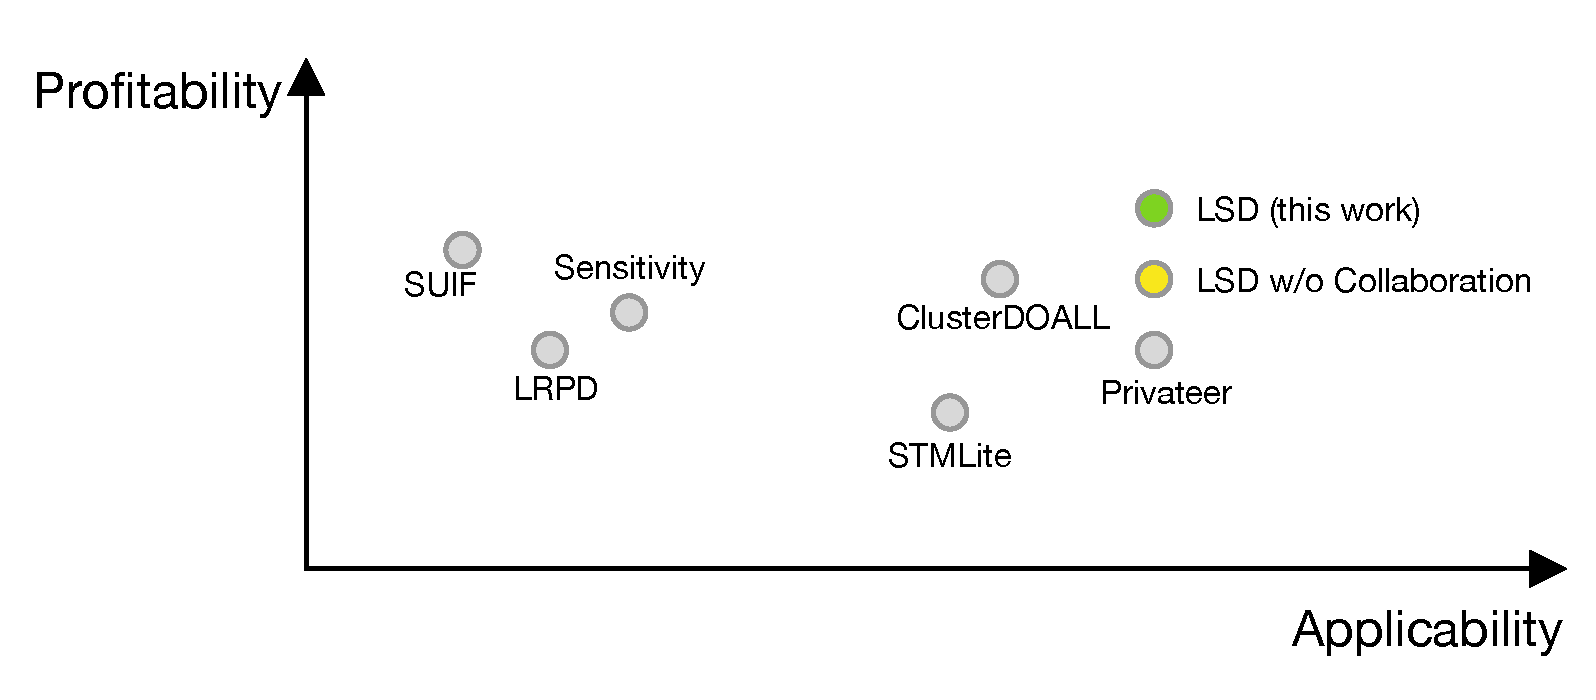
\includegraphics[width=\columnwidth]{figures/profit-appli-compare}
  \caption{Comparison of applicability and profitability.}
  \label{fig:profit-appli-compare}
\end{figure}


%Many proposals speculate low-level properties of the code, namely dependences
%between individual operations.
%%
%Such speculative systems work well when assisted by hardware
%extensions~\cite{TLS_papers...}, but yield small speedups, if any, when
%running on commodity hardware.
%%TODO: other software-spec apart from STM, more recent ones ??
%For example, Software Transactional Memories
%(STMs)~\cite{mehrara:09:stmlite} present an abstraction that facilitates
%speculating the independence of memory transactions (i.e., memory
%speculation). Validation requires logging or communication for most of the
%memory accesses within each transaction and becomes prohibitively expensive
%as the size of transaction grows.
%%
%%This reduces to comparing the read and write sets of adjacent transactions.  As
%%transactions grow, the number of memory operations within that transaction can
%%become prohibitively large. Further, instrumenting every memory operation with
%%the transaction to log or communicate every access---approximately one tenth of
%%all dynamic instructions---leads to an excessive overhead, even in the absence
%%of transaction rollbacks.
%
%%privateer
%
%%An alternative approach is to reduce memory
%
%
%Other speculative systems attempt to avoid the excessive memory speculation of
%generic transactional systems by speculating higher-level properties whose
%validation does not require logging or communication.
%%
%A prominent work of this class is Privateer~\cite{johnson:12:pldi:short}, a
%state-of-the-art Spec-DOALL parallelization system, that exhibits more
%scalable speedups compared to prior work.
%%
%Privateer partitions memory objects into several categories/families according
%to observed access patterns via profiling.  Speculating that certain
%individual memory access pairs are independent is avoided by just speculating
%separation of the families and some other simple properties.  However, detection
%of privatizable memory objects relies solely on memory and control profiling.
%Therefore, validation for a substantial set of memory objects still requires
%expensive logging and checks at every memory access, similarly to STM systems.
%% and occassional communication among workers
%%cheap spec for short-lived or read-only has also been discussed in other spec
%%systems such as cluster-doall and corD
%%

%STMLite, privateer, LRPD, ClusterDoall,
%Polaris, CorD, SUIF
%
%use of static analysis
%
%cheap spec techniques usage
%
%privatization support
%
%handling c/c++ complex data structures, pointers
%
%privatization cost
%
%reductions support
%
%scalable results (cores used)

%Table 1 compares thiswork with other existing automatic parallelization systems.
%Table ~\ref{related_work} summarizes comparison with prior work.


\subsection{Motivational example}

This work is motivated by the excessive use of memory speculation and expensive
privatization of prior speculative systems that limited their efficiency.
%
In this section, we present a code example taken from MiBench~\cite{} benchmark
dijkstra (used in the evaluation of Privateer~\cite{}) to showcase how static
analysis along with cheap-to-validate speculative assumptions can infer
high-level program properties and enable scalable parallelization.
%
We focus on two memory objects that would cause inefficiencies on prior
parallelization systems.
%
For each of these objects, we examine how we can tackle DOALL parallelization
inhibitors; in particular loop-carried memory dependences, and exhibit the
multiplicative effect of collaboration in terms of analysis accuracy.

First, a quick description of the used static and speculative analyses in our
example:
%
\begin{itemize}
%
\item \textit{Static Analysis} (see ~\cite{johnson:17:cgo} for more information)
%
  \begin{itemize}
%
  \item \textit{Alias Analysis}: an ensemble of analysis algorithms that
determine whether the footprint of an operation alias the footprint of another
operation.
%
  \item \textit{Kill-Flow}: searches for killing operations along all feasible
paths between two operations. It searches blocks which post-dominate the source
of the queried dependence and dominate the destination.
%
  \item \textit{No-Capture Source}: identifies global variables or allocators
whose address is never captured. Such objects can only be referenced through
addresses computed from the object's name. The algorithm, thus, can enumerate,
transitively, all uses of that object.
%
\end{itemize}
%
\item \textit{Speculative Analysis}
%
\begin{itemize}
%
  %\item \textit{Loop-Invariant Loaded Value Prediction}:
  \item \textit{Value Prediction Speculation~\cite{}}: identifies, using
value-prediction, profiling the predictable outcome of certain instructions.
%cite F.  Gabbay  and  A.  Mendelson.    Can  program  profiling  supportvalue
%prediction?
%
  \item \textit{Control Speculation~\cite{}}: identifies, using edge profiling,
speculatively dead code and asserts absence of memory dependences to or from
speculatively dead operations.
%cite W. Y. Chen, S. A. Mahlke, and W. W. Hwu.  Tolerating first levelmemory
%access latency in high-performance systems
%
\end{itemize}
%
\end{itemize}
%

\lstset{basicstyle=\ttfamily, numbers=left, numberstyle=\tiny,
  stepnumber=1, numbersep=5pt}
\begin{figure*}[t]
  \centering
  \scriptsize
  \subfloat[dijkstra]
  {
    \label{fig:dijkstra}
    \begin{minipage}{7.5cm}
      \begin{lstlisting}[morekeywords={iPrev,piPrev,g_qCount},belowskip=0pt]
// global variables
int iPrev;
int g_qCount = 0;

void enqueue(..., int piPrev) {
  ...
  ... = piPrev;
  g_qCount++;
}

void dequeue(..., int *piPrev) {
  if (qHead) {
    ...
    *piPrev = ...
    g_qCount--;
  }
}

for (int i = 0; i < N; i++) { // hot loop
  ...
  enqueue(i, 0, NONE);
  while ( g_qCount ) {
    dequeue(&iNode, &iDist, &iPrev);
    for (k = 0; k < NUM_NODES; k++) {
      ...
      if ( valid node ) {
        ...
        enqueue(i, iDist+iCost, iNode);
      }
    }
  }
  ...
}

\end{lstlisting}

    \end{minipage}
  }
\end{figure*}

%showcases how fine-grained collaboration between static analysis and speculative
%assumptions can infer high-level program properties without the need for
%expensive memory speculation.

%Dependence has three conditions. We say there is a memorydependence  from
%instructioni1to  instructioni2iff(alias)the footprint of operationi1may-aliasthe
%footprint ofi2, and(feasible-path) there is a feasible path of execution
%fromi1toi2which (no-kill) does not contain an operation which over-writes the
%common memory footprint. Footprint denotes theset of memory locations read or
%written by the instruction.

1) global object \textit{g\_qCount}

\textbf{Static analysis and inexpensive speculation in isolation}:
%
%Analysis Results:
Static analysis cannot disprove all loop-carried RAW and WAW dependences on
accesses of g\_qCount.
%
Profile information indicates that the first load of g\_qCount in each iteration
always returns zero.  Using this information, value prediction removes the
loop-carried RAW dependence sinking on this load.
%
Removal of this dependence prevents usage of memory speculation for this
particular load.
%
Presence of WAW dependences though necessitates privatization of the memory
object, and value prediction cannot reason about store instructions and cannot
give any additional information related to output dependences.
%
%Cost
The cost in this case includes the validation overhead for value prediction
(perform load before loop exits or on backedges and compared predicted value
with loaded value) and the privatizaition cost (monitor stores participating in
the WAW dependences to determine last written value). Bookkeping for
privatization is the dominant cost as it requires updating metadata multiple
times per loop iteration (given that some stores are within inner loops).
%dynamic resolution to determine last written value


\textbf{Collaboration of static and speculative analysis}:
%
This value prediction can be seen as a store before the first load of g\_qCount
that kills any data flow for this memory object from previous iterations.
%
An extended speculative analysis removes, similarly to the first case, the
loop-carried RAW dependence, but additionally queries alias analysis for
must-aliasing accesses with the load's address. If these accesses are dominated
by the load, then loop-carried RAW or WAW dependences from or to these accesses
can be ignored.
%
This remvoes the need to perform dynamic resolution of the last written value;
the final content of this memory location is predictable.
%any action to log (for last write) any of these individual memory operations.
%
%Interestingly, this case of privatization goes beyond the classical definition
%of privatization definition~\cite{tu-padua-array-privatization-1994}  that
%requires that every load of a privatizable element is preceded by a store to
%the element in the same iteration of the loop. In this scenario, global
%variable g\_qCount is first loaded at every iteration, a data flow exists.
%
%
The cost in this case only includes the small validation overhead for value
prediction. There is no bookkeping cost for privatization.
%
No prior work could detect and so effectively handle this new case of
privatization.
%- privatization cost: none avoid dynamic resolution to determine last written
%value (live-out value)

%TODO: use this first
2) global object \textit{iPrev}

- speculative assumption: the branch "if (qHead)" is always taken (control speculation)

- static analysis: alias analysis, killflow, noCaptureGlobal analysis passes

- validation cost: no validation cost for control spec (just misspecs if branch
  is not taken)

- Using the speculative assumption, killflow analysis can infer that the store
  in line 15 kills all other accesses of this global
variable (killed operations are identified by quering alias analysis). Given this
property, any RAW loop-carried dependence is disproved.  Additionally, static
analysis can enumerate all uses of this global, since it is not captured, and
detect that this global is used only within this loop, namely it is not a
live-out.  Thus, there is no need to log stores and keep track of the last
written value to it.

%3) TODO: example with blackscholes

For all the above memory objects, Privateer~\cite{}, the state-of-the-art DOALL
system that we mainly compare against, would require expensive logging on most
of their accesses,
%either for validation checks or for identifying who wrote last what
yielding sub-optimal speedups as clearly exhibited by our experimental results
in section ~\ref{eval}.
%all these objects are classified as privatizable by Privateer

Note that our framework is not limited to static global allocations.  It can
handle linked or recursive data structures, pointers,type  casts,  and  dynamic
allocation.

%use alvinn for value pred + alias analysis

%Note that WAR dependences can be ignored thanks to the process-based runtime
%system.


\centering
\tiny
\begin{tabular}{|c|c|c|c|c|c|c|c|c|}
  \hline
  Type of Private &
  Overlap         &
  Spec Privatization &
  Other Spec Allowed    &
  Loads Checks  &
  Store Checks    &
  Last-Write Detection &
  CoW Mapping &
  Copy-out to Main \\

%%%%%%%%%%%%%%%%%%% Shared %%%%%%%%%%%%%%%%%%%%%%%%%%
 \hline
 Shared & No & - & - & - & - & - & - & - \\
 \hline
%%%%%%%%%%%%%%%%%%% Local %%%%%%%%%%%%%%%%%%%%%%%%%%
 Local Private & Any & - & $\checkmark$ & - & - & - & $\checkmark$ & - \\
 \hline
%%%%%%%%%%%%%%%%%%% Overwrite %%%%%%%%%%%%%%%%%%%%%%%%%%
 Kill Private & Complete & - & $\checkmark$ & - & - & - & $\checkmark$ &
$\checkmark$ \\
 \hline
%%%%%%%%%%%%%%%%%%% Conservative Private %%%%%%%%%%%%%%%%%%%%%%%%%%
 Static Private & No/Partial & - & $\checkmark$ & - & - &
 $\checkmark$ & $\checkmark$ & $\checkmark$ \\
 \hline
%%%%%%%%%%%%%%%%%%% Specpriv Private %%%%%%%%%%%%%%%%%%%%%%%%%%
 Privateer Private & Any & $\checkmark$ & $\checkmark$ & $\checkmark$ & $\checkmark$ &
 $\checkmark$ & $\checkmark$ & $\checkmark$ \\
 \hline
\end{tabular}



%\lstset{basicstyle=\ttfamily, numbers=left, numberstyle=\tiny,
%  stepnumber=1, numbersep=5pt}
%\begin{figure*}[t]
%  \centering
%  \scriptsize
%  \subfloat[dijkstra -- predictable]
%  {
%    \label{fig:dijkstra}
%    \begin{minipage}{7.5cm}
%      \begin{lstlisting}[morekeywords={g_qCount},belowskip=0pt]
// predicted to be 0 at start of every iteration
int g_qCount = 0;

for ( int i = 0; int j = N/2; i < N; i++, j++ ) {
  ...
  enqueue( i, 0, NONE );
  g_qCount++;
  while ( g_qCount ) {
    dequeue( &iNode, &iDist, &iPrev );
    g_qCount--;
    for ( k = 0; k < NUM_NODES; k++ ) {
      ...
      if ( valid_node ) {
        ...
        enqueue( i, iDist + iCost, iNode );
        g_qCount++;
      }
    }
  }
  ...
}

\end{lstlisting}

%    \end{minipage}
%  }
%  \hspace{0.5cm}
%  \subfloat[dijkstra -- overwrite]
%  {
%    \label{fig:blackscholes}
%    \begin{minipage}{7.5cm}
%      \input{figures/dijkstra_overwrite_code}
%    \end{minipage}
%  }
%\end{figure*}
%
%
%
%
%\begin{figure*}[t]
%  \centering
%  \scriptsize
%  \subfloat[gemm -- shared]
%  {
%    \label{fig:gemm}
%    \begin{minipage}{7.5cm}
%      \begin{lstlisting}[escapeinside={~}{~}, belowskip=0pt]
for ( i = 0; i < ni; i++ ) {
  for ( j = 0; j < nj; j++ ) {
    C[i][j] *= beta; 
    for ( k = 0; k < nk; ++k )
      C[i][j] += alpha * A[i][k] * B[k][j];
  }
}
\end{lstlisting}

%    \end{minipage}
%  }
%  \hspace{0.5cm}
%  \subfloat[blackscholes -- overwrite]
%  {
%    \label{fig:blackscholes}
%    \begin{minipage}{7.5cm}
%      % look in Nick's motivation.tex for formatting
\begin{lstlisting}[morekeywords={prices}, belowskip=0pt]
for ( j = 0; j < NUM_RUNS; j++ ) {
  for ( i = 0; i < numOptions; i++ ) {
    prices[i] = BlkSchlsEqEuroNoDiv(
      sptprice[i], strike[i],
      rate[i], volatility[i], otime[i],
      otype[i], 0);
  }
}
\end{lstlisting}

%    \end{minipage}
%  }
%\end{figure*}
%\begin{figure*}[t]
%  \centering
%  \scriptsize
%  \subfloat[052.alvinn -- stack local]
%  {
%    \label{fig:alvinn_local}
%    \begin{minipage}{7.5cm}
%      \begin{lstlisting}[morekeywords={psum_array},belowskip=0pt]
float psum_array[NHU+1]; // stack

for (epoch = 0; epoch < NUM_EPOCHS; epoch++) {
  ...
  for ( i = 0; i < NHU+1; i++ )
    psum_array[i] = 0;
  for( i = 0; i < NOU; i++ ) {
    for ( j = 0; j < NHU+1; j++ ) {
      ...
      psum_array[j] += delta[i] * weights[i][j];
      ...
    }
  }
  for ( i = 0; i < NHU+1; i++ )
    delta[i] = hidden[i] * (1 - hidden[i]) * psum_array[i];
  ...
}
\end{lstlisting}

%    \end{minipage}
%  }
%  \hspace{0.5cm}
%  \subfloat[dijkstra -- global local]
%  {
%    \label{fig:dijkstra}
%    \begin{minipage}{7.5cm}
%      \begin{lstlisting}[morekeywords={k},belowskip=0pt]
int k;

for ( int i = 0; int j = N/2; i < N; i++, j++ ) {
  ...
  j = j%N;
  if ( i == j )
    continue;
  else {
    ...
    while ( g_qCount ) {
      ...
      for ( k = 0; k < NUM_NODES; k++ ) {
        ...
      }
    }
  }
  ...
}

\end{lstlisting}

%    \end{minipage}
%  }
%\end{figure*}

% \begin{figure*}[t]
%   \centering
%   \scriptsize
%   \subfloat[covariance -- nospec-private]
%   {
%     \label{fig:covariance}
%     \begin{minipage}{7.5cm}
%       \begin{lstlisting}[morekeywords={symmat}, belowskip=0pt]
for ( j1 = 0; j1 < m; j1++ ) {
  for ( j2 = j1; j2 < m; j2++ ) {
    symmat[j1][j2] = 0.0;
    for ( i = 0; i < n; i++ )
      symmat[j1][j2] += data[i][j1] * data[i][j2];
    symmat[j2][j1] = symmat[j1][j2];
  }
}
\end{lstlisting}

%     \end{minipage}
%   }
%   \hspace{0.5cm}
%   \subfloat[052.alvinn -- real private]
%   {
%     \label{fig:alvinn_specpriv}
%     \begin{minipage}{7.5cm}
%       \begin{lstlisting}[morekeywords={output_act}, belowskip=0pt]
float output_act[NOU];

for (epoch = 0; epoch < NUM_EPOCHS; epoch++) {
  ...
  receiver = &output_act[0];
  end_receiver = &output_act[NOU - 1];
  for ( ; receiver <= end_receiver; ) {
    *receiver = 0.0;
    sender = &hidden_act[0];
    end_sender= &hidden_act[NHU];
    for (; sender <= end_sender; )
      *receiver += (*sender++) * (*weight++);
    *receiver = SIGMOID(*receiver);
    *receiver++;
  }
  ...
  for (ou = 0; ou < NOU; ou++) {
  	delta[ou] = (teach[ou] - output_act[ou]) *
      output_act[ou] * (1.0 - output_act[ou]);
  	...
  }
  ...
}
\end{lstlisting}

%     \end{minipage}
%   }
% \end{figure*}

 %\section{Approach Overview}
\label{sec:overview}

The goal is to infer for all memory objects of each target loop high-level
properties that enable parallelization with minimal bookkeeping and access
checks.
% maybe the under which option is needed here?
%
These properties are used to group memory objects into families of objects.
%Memory objects with the same properties are grouped into the same family of
%objects.
The runtime system leverages each family's properties to maximize performance.
%
Even though, categorization of memory objects has been explored in prior
work~\cite{johnson:12:pldi, kim:12:cgo, corD},
%
the selection of properties and the assumptions under which these properties are
inferred drastically changes the parallelization profitability.  This section
explains how this work addresses these two problems more effectively than prior
work.
%to reduce speculative parallelization overheads compared to prior work.


%\subsection{Memory Object Properties}
\subsection{What Memory Object Properties?}

DOALL parallelization is \textit{applicable} when the loop's memory objects
belong to one of these categories: (i) private~\cite{privateer,LRPD} (does not
partake in any loop-carried memory flow); (ii) read-only~\cite{tian:10:pldi,
johnson:12:pldi}; (iii) local~\cite{tian:10:pldi, johnson:12:pldi,clusterDoall}
(allocated and de-allocated within the same iteration); and (iv)
reduction~\cite{privateer,LRPD_the_one_withreductionPriv} (participate in a
reduction operation only).
%

Ensuring correct live-out memory state often requires extensive bookkeeping,
during parallel execution, for the write footprint of private objects. To make
parallelization more \textit{profitable}, this work expresses more properties
for private memory objects. Private objects could additionally (a) be
independent~\cite{ARRAY_privatization} (no loop-carried false dependences); (b)
have loop-invariant condition for last update within the
loop~\cite{ARRAY_privatization}; (c) have predictable live-out content;
%(not found in prior work);
or (d) have only local accesses (allocated outside the loop, but all
accesses are contained within the loop execution).
%
%Private properties (a), (b) have been explored before in the context of static
%parallelization~\cite{ARRAY_privatization}, but never before in speculative
%parallelization systems (maybe in LRPD). No prior work leveraged property (c).
%
Table~\ref{tab:priv_types} summarizes how these properties can facilitate more
efficient parallelization compared to just inferring that a memory object is
private. In short, inference of any of these four private properties allows
complete elimination of bookkeeping and access checks. Prior software
speculative systems with extended support of privatization (Privateer~\cite{},
ClusterDoall~\cite{}) are only able to infer the simple private property and
thus always require costly checks or monitoring.

\centering
\tiny
\begin{tabular}{|c|c|c|c|c|c|c|c|c|}
  \hline
  Type of Private &
  Overlap         &
  Spec Privatization &
  Other Spec Allowed    &
  Loads Checks  &
  Store Checks    &
  Last-Write Detection &
  CoW Mapping &
  Copy-out to Main \\

%%%%%%%%%%%%%%%%%%% Shared %%%%%%%%%%%%%%%%%%%%%%%%%%
 \hline
 Shared & No & - & - & - & - & - & - & - \\
 \hline
%%%%%%%%%%%%%%%%%%% Local %%%%%%%%%%%%%%%%%%%%%%%%%%
 Local Private & Any & - & $\checkmark$ & - & - & - & $\checkmark$ & - \\
 \hline
%%%%%%%%%%%%%%%%%%% Overwrite %%%%%%%%%%%%%%%%%%%%%%%%%%
 Kill Private & Complete & - & $\checkmark$ & - & - & - & $\checkmark$ &
$\checkmark$ \\
 \hline
%%%%%%%%%%%%%%%%%%% Conservative Private %%%%%%%%%%%%%%%%%%%%%%%%%%
 Static Private & No/Partial & - & $\checkmark$ & - & - &
 $\checkmark$ & $\checkmark$ & $\checkmark$ \\
 \hline
%%%%%%%%%%%%%%%%%%% Specpriv Private %%%%%%%%%%%%%%%%%%%%%%%%%%
 Privateer Private & Any & $\checkmark$ & $\checkmark$ & $\checkmark$ & $\checkmark$ &
 $\checkmark$ & $\checkmark$ & $\checkmark$ \\
 \hline
\end{tabular}




%\subsection{How to Classify?}
%\subsection{How to Infer Memory Object Properties \\ Without Expensive Runtime
%Costs?}
\subsection{How to Infer Memory Object Properties?}

%Classifying memory objects
Characterizing the behavior of memory objects requires
%(i) identification of accesses to this object within the loop and
(i) mapping memory accesses to objects and (ii) analysis of the dependences that
these accesses introduce.
% characterize accesses
This work attempts to satisfy these two requirements by using a combination of
cheap-to-validate speculative assumptions and static analysis. For almost all
the memory objects of the evaluated benchmarks, this combination was sufficient
and no use of memory speculation or expensive bookkeeping was required.

%\paragraph{Determine accesses of memory objects:}
\paragraph{Map accesses to underlying memory objects:}
%
Static analysis can handle this problem for several cases of statically
allocated objects.
%
However, this task often becomes too challenging for static analysis for
general-purpose programs with unrestricted pointers, dynamic allocation, and
type casts.
%
%Briefly, this task entails ...  Challenges include points-to mapping from
%pointers to memory objects, different objects created by the same static
%instruction, unrestricted pointers presence of ``disguised''
%pointers~\cite{citation3_from_privateer}.  (not all pointer values are
%necessarily visible in the IR).
%
%These challenges often necessitate use of speculation.
Thus, in some cases use of speculation is necessary.
%
A points-to profiler can identify this mapping of memory accesses to underlying
memory objects.
%
Validating this points-to profiling information at the memory object granularity
would be expensive.
%instead of checking at runtime that each individual memory access points to the
%correct set of underlying objects,
%
%To enable cheap validation, it groups together memory objects with the same
%access pattern to a few heaps and only validates at runtime the correctness of
%points-to heap mapping.
%
% To reduce sensitivity to memory layout, Privateer speculativelyseparates
% memory objects
%
Same as in Privateer~\cite{johnson:pldi:12}, since all memory objects of the
same family share the same properties, inexpensive points-to family validation
is sufficient.
%
%TODO: maybe add one extra sentence here to explain why it is called separation
%spec or explain it more
%Inexpensive checks with neither bookkeeping nor inter-worker communication
%ensure that all accesses point to the correct heap.
%
%For example, the read-only family contains objects that speculatively map to
%read-only memory operations.  namely all the memory access have the read-only
%property.
%
This speculative scheme is called separation speculation.
%
%In contrast with Privateer~\cite{johnson:pldi:12}, we decouple separation
%speculation from characterizing memory accesses.
Note that Privateer's monolithic design of classification entangles separation
speculation with memory speculation and other profiling-based information
resulting in high runtime overhead (see section~\ref{eval}).
%
In contrast with Privateer, this work employs a modular design where separation
speculation is decoupled and can be used in conjunction with any other
cheap-to-validate speculation or static analysis to infer memory object
properties. This modularity leads to better planning and selection of minimum
cost solutions.

\paragraph{Dependence Analysis:}

%
Traditionally, dependence analysis (static, dynamic or speculative) in
speculative parallelization only attempts to completely remove dependences.
%
If a dependence cannot be removed even with usage of speculation, because
it is a real dependence that frequently manifests at runtime, no useful
information is provided related to this dependence.
%
Static analysis though, even if it failed to disprove a dependence, could
still infer some useful property for this dependence or the dependent
instructions.
TODO: briefly mention cases of annotations or nothing
Mention static analysis and speculative techniques used to annotate edges
or vertices

%Combining static with cheap-to-validate speculative analysis also
%enables property inference for efficient privatization.
%%
%Prior parallelization systems
%%~\cite{smtlite:09:pldi, kim:12:cgo, johnson:17:cgo}
%use static analysis or speculation mainly to remove memory
%dependences.  Sometimes though some dependences are real and cannot be
%removed via any kind of analysis.
%%For example,
%In particular, reuse of data structures creates cross-iteration false
%(output and anti) memory dependences.
%%
%In this scenario, analysis passes and speculative information can
%still express some useful properties for these dependences or the
%dependent instructions.  This partial information can be combined to
%infer a higher level property that enables more efficient
%parallelization.
%
%% isn't that what transformation do anyway? query analysis for
%% properties?  but we present a structured way to express that?  how
%% do analysis know what's useful.


%gives info to transforamtion.
%maybe in conjuction with other info from other analysis can enable a
%transformation efficiently
%some information that could enable a transformation enable more
%efficient parallelization

Explain inference of properties. Move that to next section.

One such property
that is explored in this paper is related to output dependences.  We refer
to this property as \textit{overwrite} and it expresses that the
destination operation of the dependence overwrites, in every iteration of
the target loop, the write footprint of the source operation.
%
%This information in conjunction with other static or speculative
%information infers that a private object has the property of
%loop-invariant condition for last update.
If all dependences related to a private object have the \textit{overwrite}
property then the private object has loop-invariant condition for last
update. In this case the last executed iteration has the correct live-out
memory state for this object and thus there is no need to monitor writes
for this memory object.

Maybe some of this info should be mention in the next section.
HERE briefly mention all the options.
Mention overwrite in the example subsection maybe


Value prediction can detect memory locations with loop-invariant values.
Not just remove dependences, add the annotation and remove cost of
monitoring wrties.
Loaded value re-interpreted as a store and kills all other RAW.

Independent can be infered by just disproving all output dependences. This
proves that there is no overlapping of writes.


Regarding dependence removal, prior work only used static analysis and
speculative assumptions in a sequence, operating independently of each
other.
%
This work suggests that exposing cheap-to-validate speculative assumptions
to static analysis can enable removal of memory dependences that would
otherwise require memory speculation.
TODO: add examples here
Figure out when to mention details about forms of collab. Probably in the
next section. Here just mention the techniques involved

For more details refer to section~\ref{collab}.


%Prior work only attempted to use static analysis and speculative assumptions
%separately to remove different dependences. If static analysis or speculative
%assumptions are unable to remove a dependence on their own, then there no
%collaboration between static analysis nor partial info to be used by
%transformations.


%In the past, privateer monolithically combined separation logic with
%mem spec to infer properties.
%no usage of static analusos/

%Mention the two speculative ones
%plus the usage of separation logic
%and the rest are the analysis algorithms from CAF


%First, a quick description of the used static and speculative analyses in our
%example:
%%
%\begin{itemize}
%%
%\item \textit{Static Analysis} (see ~\cite{johnson:17:cgo} for more information)
%%
%  \begin{itemize}
%%
%  \item \textit{Alias Analysis}: an ensemble of analysis algorithms that
%determine whether the footprint of an operation alias the footprint of another
%operation.
%%
%  \item \textit{Kill-Flow}: searches for killing operations along all feasible
%paths between two operations. It searches blocks which post-dominate the source
%of the queried dependence and dominate the destination.
%%
%  \item \textit{No-Capture Source}: identifies global variables or allocators
%whose address is never captured. Such objects can only be referenced through
%addresses computed from the object's name. The algorithm, thus, can enumerate,
%transitively, all uses of that object.
%%
%\end{itemize}
%%
%\item \textit{Speculative Analysis}
%%
%\begin{itemize}
%%
%  %\item \textit{Loop-Invariant Loaded Value Prediction}:
%  \item \textit{Value Prediction Speculation~\cite{}}: identifies, using
%value-prediction, profiling the predictable outcome of certain instructions.
%%cite F.  Gabbay  and  A.  Mendelson.    Can  program  profiling  supportvalue
%%prediction?
%%
%  \item \textit{Control Speculation~\cite{}}: identifies, using edge profiling,
%speculatively dead code and asserts absence of memory dependences to or from
%speculatively dead operations.
%%cite W. Y. Chen, S. A. Mahlke, and W. W. Hwu.  Tolerating first levelmemory
%%access latency in high-performance systems
%%
%\end{itemize}
%%
%\end{itemize}
%%

%Private detection requires privatization criteria and actual detection.

%conditional update makes it hard to find last store
%  but in some cases ctrl spec can be used to remove this problem!
%and remove RAW and allow cheap privitization


\lstset{basicstyle=\ttfamily, numbers=left, numberstyle=\tiny,
  stepnumber=1, numbersep=5pt}

\begin{figure*}
\centering
\subfloat[Privateer~\cite{johnson:12:pdli}]{
  \centering
  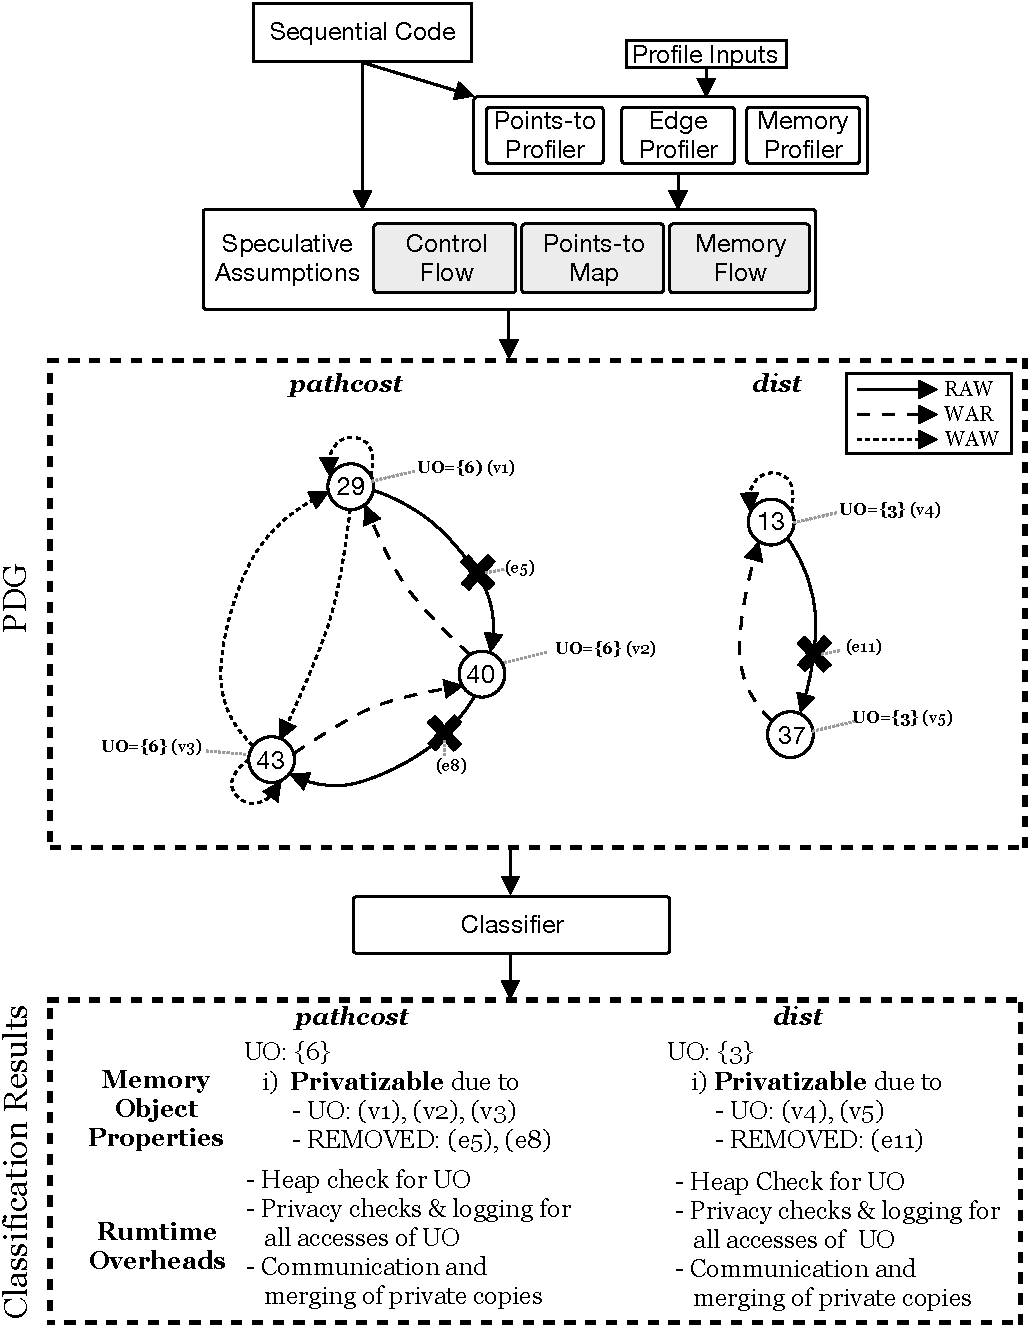
\includegraphics[width=0.46\textwidth]{figures/privateer-example-crop}
}
\qquad
\subfloat[This work]{
  \centering
  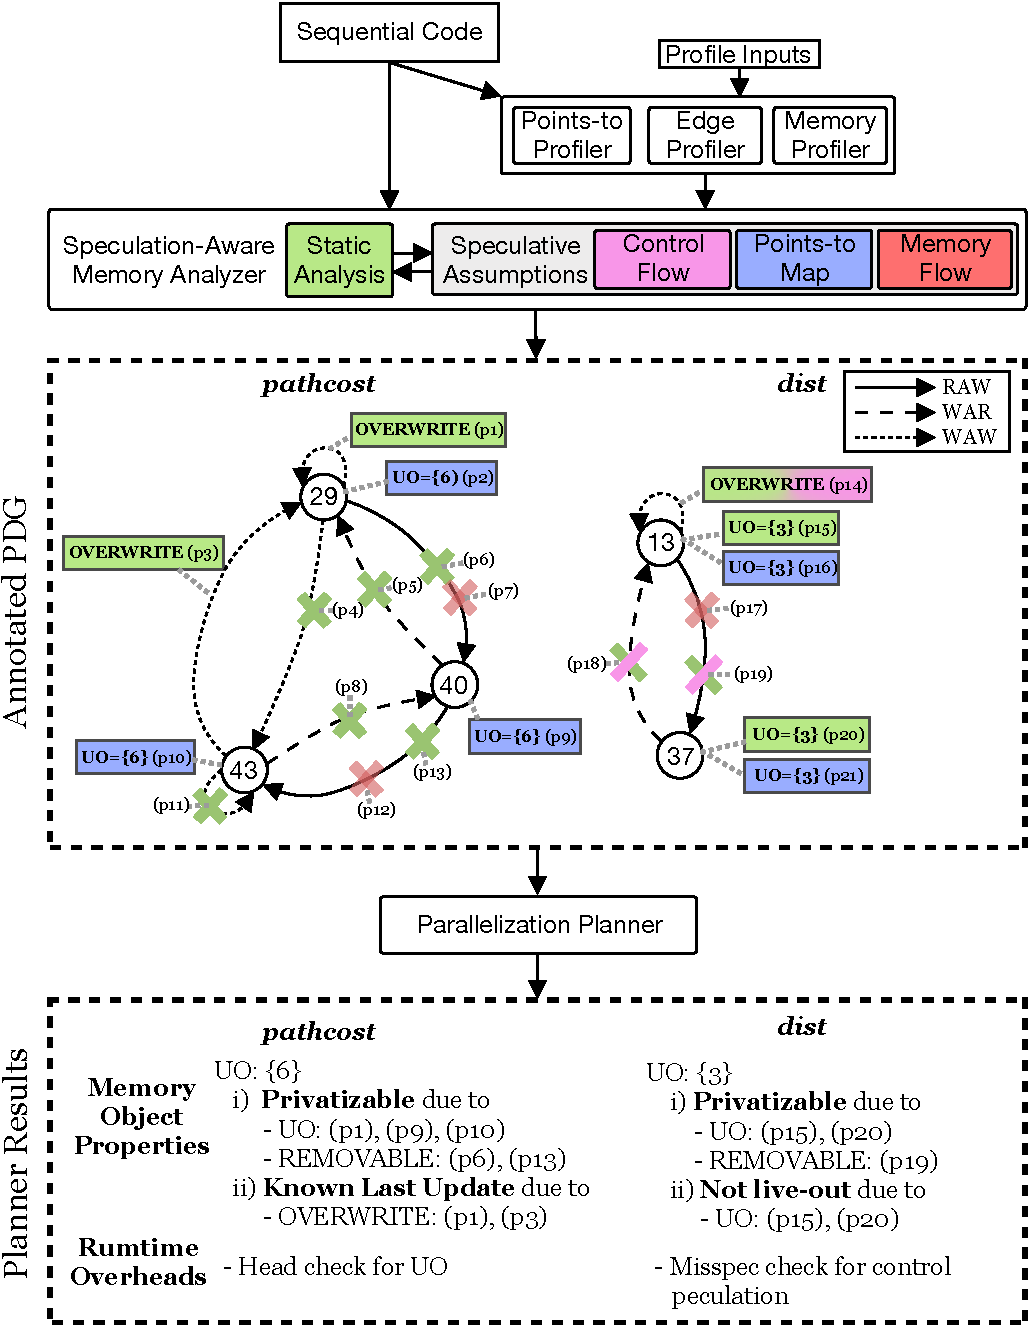
\includegraphics[width=0.46\textwidth]{figures/perspective-example-crop}
}
\caption{Property inference comparison of Privateer with LSD for memory
objects \textit{pathcost} and \textit{dist} of the hot loop of \textit{dijkstra}}
\label{fig:dijkstra_motivation_comparison}
\end{figure*}

\begin{figure*}
\centering
\scriptsize
\subfloat[Privateer~\cite{johnson:12:pdli}]{
  \centering
  \begin{minipage}{8.55cm}
  \begin{lstlisting}[morekeywords={pathcost}, belowskip=0pt, firstnumber=1,
name=dij_checks]
int *pathcost; // dyn alloc 1-D N
int *adj; // dyn alloc 2-D NxN
int dist, v, src, i;

for (src=0; src<N; src++) {
\end{lstlisting}

\begin{lstlisting}[morekeywords={pathcost}, aboveskip=0pt,belowskip=0pt,backgroundcolor=\color{lightgray},
firstnumber=auto, name=dij_checks]
  // Privacy Check
  private_write(pathcost, N*sizeof(int));
\end{lstlisting}

\begin{lstlisting}[morekeywords={pathcost},aboveskip=0pt, belowskip=0pt, firstnumber=auto,name=dij_checks]
  for (i=0; i<N; i++)
    pathcost[i] = inf;

  enqueue(src, 0);
  while (!emptyQ()) {
    dequeue(&v, &dist);
    for (i=0; i<N; i++) {
      nDist = adj[v][i] + dist;
\end{lstlisting}

\begin{lstlisting}[morekeywords={pathcost}, aboveskip=0pt,belowskip=0pt,backgroundcolor=\color{lightgray},
firstnumber=auto, name=dij_checks]
      // Privacy Check
      private_read(pathcost, sizeof(int));
\end{lstlisting}


\begin{lstlisting}[morekeywords={pathcost}, aboveskip=0pt, belowskip=0pt, firstnumber=auto,name=dij_checks]
      if (pathcost[i] > nDist) {
\end{lstlisting}

\begin{lstlisting}[morekeywords={pathcost}, aboveskip=0pt,belowskip=0pt,backgroundcolor=\color{lightgray},
firstnumber=auto, name=dij_checks]
        // Privacy Check
        private_write(pathcost, sizeof(int));
\end{lstlisting}

\begin{lstlisting}[morekeywords={pathcost}, aboveskip=0pt, belowskip=0pt, firstnumber=auto,name=dij_checks]
        pathcost[i] = nDist;
        enqueue(i, nDist);
      }
    }
  }
}
\end{lstlisting}

  \end{minipage}
}
\qquad
\qquad
\subfloat[This work]{
  \centering
  \begin{minipage}{7.2cm}
  %\begin{lstlisting}[morekeywords={pathcost}, belowskip=0pt, firstnumber=1,
%name=dij_checks]
%int *pathcost; // dyn alloc 1-D N
%int *adj; // dyn alloc 2-D NxN
%int dist, v, src, i;


\begin{lstlisting}[morekeywords={pathcost,dist}, belowskip=0pt,
firstnumber=10, name=dij_checks, showlines=true]
int dequeue() {
  if (!emptyQ()) {


\end{lstlisting}

\begin{lstlisting}[morekeywords={pathcost,dist}, aboveskip=0pt, belowskip=0pt,
firstnumber=13, name=dij_checks]
    dist = ...
    ...
  }
\end{lstlisting}

  \begin{lstlisting}[morekeywords={pathcost}, aboveskip=0pt,belowskip=0pt,backgroundcolor=\color{lightgray}, firstnumber=auto, name=dij_checks]
  else // 0% added overhead
    misspec("Control misspec in dequeue()");
\end{lstlisting}

\begin{lstlisting}[morekeywords={pathcost,dist}, aboveskip=0pt, belowskip=0pt,
firstnumber=auto, name=dij_checks,showlines=true]
}

void worker_loop(int start, int N, int step) {

\end{lstlisting}

  \begin{lstlisting}[morekeywords={pathcost}, aboveskip=0pt,belowskip=0pt,backgroundcolor=\color{lightgray},
  firstnumber=auto, name=dij_checks,showlines=true]
  // Separation Local Check -- < 0.001% added overhead
  check_heap(pathcost, OVERWRITE_PRIVATE);
  \end{lstlisting}

\begin{lstlisting}[morekeywords={pathcost}, aboveskip=0pt,
belowskip=0pt, firstnumber=24,name=dij_checks,showlines=true]

  for (src=start; src<N; src+=step) {


\end{lstlisting}
\begin{lstlisting}[morekeywords={pathcost,dist}, aboveskip=0pt,
belowskip=0pt, firstnumber=28,name=dij_checks,showlines=true]
    for (i=0; i<N; i++)
      pathcost[i] = inf;

    enqueue(src, 0);
    while (!emptyQ()) {
      int v = dequeue();
      for (i=0; i<N; i++) {
\end{lstlisting}
\begin{lstlisting}[morekeywords={pathcost,dist,nDist}, aboveskip=0pt,
belowskip=0pt, firstnumber=auto,name=dij_checks,showlines=true]



        nDist = adj[v][i] + dist;
\end{lstlisting}
\begin{lstlisting}[morekeywords={pathcost}, aboveskip=0pt,
belowskip=0pt, firstnumber=auto,name=dij_checks,showlines=true]


        if (pathcost[i] > nDist) {


\end{lstlisting}
\begin{lstlisting}[morekeywords={pathcost}, aboveskip=0pt,
belowskip=0pt, firstnumber=auto,name=dij_checks]
          pathcost[i] = nDist;
          enqueue(i, nDist);
        }
      }
    }
\end{lstlisting}

\begin{lstlisting}[morekeywords={pathcost,dist}, aboveskip=0pt,
belowskip=0pt, firstnumber=auto,name=dij_checks,showlines=true]
  }
\end{lstlisting}

\begin{lstlisting}[morekeywords={pathcost},
aboveskip=0pt,belowskip=0pt,backgroundcolor=\color{lightgray},
firstnumber=auto, name=dij_checks,showlines=true]
  // only last iter's pathcost array
  // needs to be communicated -- < 1% added overhead
  if (src == N-1+step)
    communicate_pathcost();
\end{lstlisting}

\begin{lstlisting}[morekeywords={pathcost}, aboveskip=0pt,
belowskip=0pt, firstnumber=auto,name=dij_checks]
}
\end{lstlisting}

  \end{minipage}
}
\caption{Source code comparison of Privateer with LSD for parallelized hot loop
of \textit{dijkstra}. Checkpointing occurs every several (long running) loop iterations, thus its
overhead is negligeable for \textit{dijkstra}. Logging and checks
during loop execution dominate the overheads.}
\label{fig:dijkstra_motivation_comparison_source_code}
\end{figure*}



\paragraph{Example:}
This example underlines inefficiencies and limitations of prior work and
showcases how the combination of static analysis with cheap-to-validate
speculative assumptions can infer program properties that enable scalable
parallelization.
%
Consider the code in
Figure~\ref{fig:dijkstra_motivation} (taken from MiBench~\cite{} benchmark
dijkstra, used in the evaluation of Privateer~\cite{}).
%
Reuse across iterations of the \textbf{pathcost} array and global variable
\textbf{dist} creates cross-iteration false dependences that inhibit
parallelization.
%
Privatization enables parallelization of this loop by creating private
copies of \textbf{pathcost} and \textbf{dist} memory objects for every
worker.
%
From prior work, Privateer~\cite{johnson:12:pldi} is the only automatic
system to support privatization of dynamically allocated objects, like
\textbf{pathcost}, even in the presence of unrestricted pointers.
%
Figure~\ref{fig:dijkstra_motivation_comparison} compares the property
inference property of Privateer compared to this work.
The difference is that

Figure~\ref{fig:dijkstra_motivation_comparison_source_code} compares the
resulting parallelized versions (in a simplified form) for Privateer and
this work. The code includes all the added checks, logging and handling
live-out overheads. The code changes are marked with the average added
overhead over the useful work of each worker.
It is clear that Privateer introduces a lot of added overhead considerably
limiting its profitability. XXX on the other side ..


Privateer would choose to just do simple privatization with mem spec.
The spec-aware analyzer allows removal of mem spec and efficient
privatization in this case.

\begin{itemize}
\item
Privatization of these memory objects requires:
\begin{enumerate}
\item
identification of all accesses of these objects
    within the loop
\item
absence of cross-iteration flow
     dependences on each of these accesses
\end{enumerate}

\end{itemize}


Remove text from figure 1. Just add some here, the rest has been explained
earlier.
Real dependnecs prevent
DOALL can become applicable if these two objects are proven to have the
private property.

We compare our approach where we combine static analysis with cheap-to-validate
with privateer's monolithic approach that over-speculates and is limited by high
runtime overheads.

We initially present the compilation flow for both approaches, then the
resulting parallelized code and finally the flow of live-in and live-out memory
data.

Whilst the private property is enough for DOALL
Notice that we infer an additional property that improves the profitability
of parallelization.

%Note that anti-dependences are ignored since both systems use
%process-based runtime systems.

For inferring the property that a memory object has the locally-accessed
property, it suffices to identify all accesses of the memory object. If all
these accesses are within the loop then the memory object has the
locally-accessed property.


%dijkstra (used in the evaluation of Privateer~\cite{}) to showcase how static
%analysis along with cheap-to-validate speculative assumptions can infer
%high-level program properties and enable scalable parallelization.
%%
%We focus on two memory objects that would cause inefficiencies on prior
%parallelization systems.
%%
%For each of these objects, we examine how we can tackle DOALL parallelization
%inhibitors; in particular loop-carried memory dependences, and exhibit the
%multiplicative effect of collaboration in terms of analysis accuracy.
%


%%showcases how fine-grained collaboration between static analysis and speculative
%%assumptions can infer high-level program properties without the need for
%%expensive memory speculation.
%
%%Dependence has three conditions. We say there is a memorydependence  from
%%instructioni1to  instructioni2iff(alias)the footprint of operationi1may-aliasthe
%%footprint ofi2, and(feasible-path) there is a feasible path of execution
%%fromi1toi2which (no-kill) does not contain an operation which over-writes the
%%common memory footprint. Footprint denotes theset of memory locations read or
%%written by the instruction.
%
%1) global object \textit{g\_qCount}
%
%\textbf{Static analysis and inexpensive speculation in isolation}:
%%
%%Analysis Results:
%Static analysis cannot disprove all loop-carried RAW and WAW dependences on
%accesses of g\_qCount.
%%
%Profile information indicates that the first load of g\_qCount in each iteration
%always returns zero.  Using this information, value prediction removes the
%loop-carried RAW dependence sinking on this load.
%%
%Removal of this dependence prevents usage of memory speculation for this
%particular load.
%%
%Presence of WAW dependences though necessitates privatization of the memory
%object, and value prediction cannot reason about store instructions and cannot
%give any additional information related to output dependences.
%%
%%Cost
%The cost in this case includes the validation overhead for value prediction
%(perform load before loop exits or on backedges and compared predicted value
%with loaded value) and the privatizaition cost (monitor stores participating in
%the WAW dependences to determine last written value). Bookkeping for
%privatization is the dominant cost as it requires updating metadata multiple
%times per loop iteration (given that some stores are within inner loops).
%%dynamic resolution to determine last written value
%
%
%\textbf{Collaboration of static and speculative analysis}:
%%
%This value prediction can be seen as a store before the first load of g\_qCount
%that kills any data flow for this memory object from previous iterations.
%%
%An extended speculative analysis removes, similarly to the first case, the
%loop-carried RAW dependence, but additionally queries alias analysis for
%must-aliasing accesses with the load's address. If these accesses are dominated
%by the load, then loop-carried RAW or WAW dependences from or to these accesses
%can be ignored.
%%
%This remvoes the need to perform dynamic resolution of the last written value;
%the final content of this memory location is predictable.
%%any action to log (for last write) any of these individual memory operations.
%%
%%Interestingly, this case of privatization goes beyond the classical definition
%%of privatization definition~\cite{tu-padua-array-privatization-1994}  that
%%requires that every load of a privatizable element is preceded by a store to
%%the element in the same iteration of the loop. In this scenario, global
%%variable g\_qCount is first loaded at every iteration, a data flow exists.
%%
%%
%The cost in this case only includes the small validation overhead for value
%prediction. There is no bookkeping cost for privatization.
%%
%No prior work could detect and so effectively handle this new case of
%privatization.
%%- privatization cost: none avoid dynamic resolution to determine last written
%%value (live-out value)
%
%%TODO: use this first
%2) global object \textit{iPrev}
%
%- speculative assumption: the branch "if (qHead)" is always taken (control speculation)
%
%- static analysis: alias analysis, killflow, noCaptureGlobal analysis passes
%
%- validation cost: no validation cost for control spec (just misspecs if branch
%  is not taken)
%
%- Using the speculative assumption, killflow analysis can infer that the store
%  in line 15 kills all other accesses of this global
%variable (killed operations are identified by quering alias analysis). Given this
%property, any RAW loop-carried dependence is disproved.  Additionally, static
%analysis can enumerate all uses of this global, since it is not captured, and
%detect that this global is used only within this loop, namely it is not a
%live-out.  Thus, there is no need to log stores and keep track of the last
%written value to it.
%
%%3) TODO: example with blackscholes
%
%For all the above memory objects, Privateer~\cite{}, the state-of-the-art DOALL
%system that we mainly compare against, would require expensive logging on most
%of their accesses,
%%either for validation checks or for identifying who wrote last what
%yielding sub-optimal speedups as clearly exhibited by our experimental results
%in section ~\ref{eval}.
%%all these objects are classified as privatizable by Privateer
%
%Note that our framework is not limited to static global allocations.  It can
%handle linked or recursive data structures, pointers,type  casts,  and  dynamic
%allocation.
%
%%use alvinn for value pred + alias analysis
%
%%Note that WAR dependences can be ignored thanks to the process-based runtime
%%system.


%\lstset{basicstyle=\ttfamily, numbers=left, numberstyle=\tiny,
%  stepnumber=1, numbersep=5pt}
%\begin{figure*}[t]
%  \centering
%  \scriptsize
%  \subfloat[dijkstra -- predictable]
%  {
%    \label{fig:dijkstra}
%    \begin{minipage}{7.5cm}
%      \begin{lstlisting}[morekeywords={g_qCount},belowskip=0pt]
// predicted to be 0 at start of every iteration
int g_qCount = 0;

for ( int i = 0; int j = N/2; i < N; i++, j++ ) {
  ...
  enqueue( i, 0, NONE );
  g_qCount++;
  while ( g_qCount ) {
    dequeue( &iNode, &iDist, &iPrev );
    g_qCount--;
    for ( k = 0; k < NUM_NODES; k++ ) {
      ...
      if ( valid_node ) {
        ...
        enqueue( i, iDist + iCost, iNode );
        g_qCount++;
      }
    }
  }
  ...
}

\end{lstlisting}

%    \end{minipage}
%  }
%  \hspace{0.5cm}
%  \subfloat[dijkstra -- overwrite]
%  {
%    \label{fig:blackscholes}
%    \begin{minipage}{7.5cm}
%      \input{figures/dijkstra_overwrite_code}
%    \end{minipage}
%  }
%\end{figure*}
%
%
%
%
%\begin{figure*}[t]
%  \centering
%  \scriptsize
%  \subfloat[gemm -- shared]
%  {
%    \label{fig:gemm}
%    \begin{minipage}{7.5cm}
%      \begin{lstlisting}[escapeinside={~}{~}, belowskip=0pt]
for ( i = 0; i < ni; i++ ) {
  for ( j = 0; j < nj; j++ ) {
    C[i][j] *= beta; 
    for ( k = 0; k < nk; ++k )
      C[i][j] += alpha * A[i][k] * B[k][j];
  }
}
\end{lstlisting}

%    \end{minipage}
%  }
%  \hspace{0.5cm}
%  \subfloat[blackscholes -- overwrite]
%  {
%    \label{fig:blackscholes}
%    \begin{minipage}{7.5cm}
%      % look in Nick's motivation.tex for formatting
\begin{lstlisting}[morekeywords={prices}, belowskip=0pt]
for ( j = 0; j < NUM_RUNS; j++ ) {
  for ( i = 0; i < numOptions; i++ ) {
    prices[i] = BlkSchlsEqEuroNoDiv(
      sptprice[i], strike[i],
      rate[i], volatility[i], otime[i],
      otype[i], 0);
  }
}
\end{lstlisting}

%    \end{minipage}
%  }
%\end{figure*}
%\begin{figure*}[t]
%  \centering
%  \scriptsize
%  \subfloat[052.alvinn -- stack local]
%  {
%    \label{fig:alvinn_local}
%    \begin{minipage}{7.5cm}
%      \begin{lstlisting}[morekeywords={psum_array},belowskip=0pt]
float psum_array[NHU+1]; // stack

for (epoch = 0; epoch < NUM_EPOCHS; epoch++) {
  ...
  for ( i = 0; i < NHU+1; i++ )
    psum_array[i] = 0;
  for( i = 0; i < NOU; i++ ) {
    for ( j = 0; j < NHU+1; j++ ) {
      ...
      psum_array[j] += delta[i] * weights[i][j];
      ...
    }
  }
  for ( i = 0; i < NHU+1; i++ )
    delta[i] = hidden[i] * (1 - hidden[i]) * psum_array[i];
  ...
}
\end{lstlisting}

%    \end{minipage}
%  }
%  \hspace{0.5cm}
%  \subfloat[dijkstra -- global local]
%  {
%    \label{fig:dijkstra}
%    \begin{minipage}{7.5cm}
%      \begin{lstlisting}[morekeywords={k},belowskip=0pt]
int k;

for ( int i = 0; int j = N/2; i < N; i++, j++ ) {
  ...
  j = j%N;
  if ( i == j )
    continue;
  else {
    ...
    while ( g_qCount ) {
      ...
      for ( k = 0; k < NUM_NODES; k++ ) {
        ...
      }
    }
  }
  ...
}

\end{lstlisting}

%    \end{minipage}
%  }
%\end{figure*}

% \begin{figure*}[t]
%   \centering
%   \scriptsize
%   \subfloat[covariance -- nospec-private]
%   {
%     \label{fig:covariance}
%     \begin{minipage}{7.5cm}
%       \begin{lstlisting}[morekeywords={symmat}, belowskip=0pt]
for ( j1 = 0; j1 < m; j1++ ) {
  for ( j2 = j1; j2 < m; j2++ ) {
    symmat[j1][j2] = 0.0;
    for ( i = 0; i < n; i++ )
      symmat[j1][j2] += data[i][j1] * data[i][j2];
    symmat[j2][j1] = symmat[j1][j2];
  }
}
\end{lstlisting}

%     \end{minipage}
%   }
%   \hspace{0.5cm}
%   \subfloat[052.alvinn -- real private]
%   {
%     \label{fig:alvinn_specpriv}
%     \begin{minipage}{7.5cm}
%       \begin{lstlisting}[morekeywords={output_act}, belowskip=0pt]
float output_act[NOU];

for (epoch = 0; epoch < NUM_EPOCHS; epoch++) {
  ...
  receiver = &output_act[0];
  end_receiver = &output_act[NOU - 1];
  for ( ; receiver <= end_receiver; ) {
    *receiver = 0.0;
    sender = &hidden_act[0];
    end_sender= &hidden_act[NHU];
    for (; sender <= end_sender; )
      *receiver += (*sender++) * (*weight++);
    *receiver = SIGMOID(*receiver);
    *receiver++;
  }
  ...
  for (ou = 0; ou < NOU; ou++) {
  	delta[ou] = (teach[ou] - output_act[ou]) *
      output_act[ou] * (1.0 - output_act[ou]);
  	...
  }
  ...
}
\end{lstlisting}

%     \end{minipage}
%   }
% \end{figure*}

 \section{The \name Approach}
\label{sec:approach}

Current parallelizing compiler designs force code analyses, transformations, and speculative techniques to work as a pipeline.
This design excludes the possibility of non-linear and fine-grain interactions between them, which makes important parallelization opportunities unreachable.
To overcome this limitation, \name introduces a compiler design where static code analyses and speculation techniques are tightly coupled to boost their discovery of parallelization opportunities (section~\ref{analyzer}).
This tight interaction generates information in the form of a dependence graph annotated with speculative assumptions.
\namensp's design also tightly couples code transformations with speculative assumptions to drastically reduce the overhead of the formers (section~\ref{enablers}).
%These tight integrations are accomplished introducing new interfaces between compilation passes (section~\ref{enablers}) that enable their non-linear and fine-grained interactions.
These new interfaces create extra degrees of freedom, which enable \name to realize many new parallelization opportunities reaching the applicability of speculation-based approaches with the efficiency of static analyses ones.

%\name combines a speculation-aware memory analyzer, enabling
%transformations including efficient speculative privatization, and a
%parallelization planner into an exploration phase designed to find the
%best performing set of parallelization techniques.  This section
%discusses the main contributions of this paper
%(sections~\ref{analyzer},\ref{enablers},\ref{planner}), and
%presents a code example (section~\ref{motiv_example}) to underline
%improvements over Privateer~\cite{johnson:12:pldi}, a state-of-the-art
%speculative DOALL parallelization system.

\subsection{Planning}
%
Unlike prior speculative systems that apply a sequence of
parallelization-enabling transforms in a fixed order, \name proposes a
more sensible approach: before applying any transformation, plan
first.

Enabling transforms modify the code to remove parallelization
inhibitors, which in the context of DOALL parallelization are
cross-iteration dependences.
%
To facilitate planning, all transformations are split into two parts.
The applicability guard that participates in the planning phase of the
compilation and the actual transformation that is applied, if
selected, in the transformation phase.
%This separation of decision making and application of transformations
%allows \name to carefully select the most profitable plan.
The applicability guard utilizes properties produced by memory
analysis and speculative assumptions\footnote{We define speculative
assumptions as predictions of program properties based on profile
information.} to determine which parallelization inhibitors the
corresponding transform can handle.
%
The interface between memory analysis and speculative assumptions, and
enabling transforms is an annotated with properties program dependence
graph (PDG).
%
%The used speculative assumptions would need to be validated at
%runtime for the transformation to be correct.
%
The output of each applicability guard is collected in a
transformation proposal which is sent to the planner.
%
%The effect of each enabling transform is collected in a
%transformation proposal.
%
The proposal also includes a cost for the application of the
transformation itself and a set of speculative assumptions required
for the transformation to be applicable and correct.

Memory-related transformations instead of targeting cross-iteration
dependences, offer to handle a set of memory objects, in effect
addressing all their cross-iteration dependences. This object-centric
approach is motivated by the fact that memory-related enabling
transformations often operate at an object level. For example, the
privatization transformation create private copies of memory objects.

\paragraph{Planner}

%The input to the planner is a program dependence graph and
%transformation proposals of the enabling transformations.
%
The output of the planner is the best performing set of
transformations that addresses all the parallelization inhibitors.
%
The planner is able to perform global reasoning by centralizing the
currently decentralized and greedy decision-making process found in
prior parallelizing compilers.
%
The generated plan includes a set of enabling transformations and a
set of transformations for validating speculative assumptions.
%
These are the transformations that are applied at the transformation
phase of compilation.

\subsection{Speculation-Aware Memory Analyzer}

Prior techniques use memory analysis and speculative assumptions
independently.  Instead, this work proposes a speculation-aware memory
analyzer that combines the strengths of static analysis and
cheap-to-validate speculative assumptions to reduce the need for
expensive speculation.  If memory analysis fails on its own to resolve
an analysis query, it interprets cheap-to-validate speculative
assumptions as facts ignoring the possibility of misspeculation.
%
The inclusion of speculation changes the semantics of traditional
memory analysis. It is now required to specify for each answer the
speculative assumptions, if any, that were used in the process.
%
Just applying speculation and then querying memory analysis again
would not have the same effect since the possibility of misspeculation
restrains static analysis. For more details regarding
speculation-aware memory analysis see \cref{sama}.

\subsection{New Enabling Transformations}

%Either all static, all speculation.
Prior work on speculative parallelization often focuses on the
enabling effect of transformations without considering their cost.  To
maximize applicability, enabling transforms are often given a program
dependence structure relaxed with the use of all the available
speculative assumptions.  This approach not only creates ambiguity in
terms of what speculative assumptions are necessary but also prevents
usage of efficient variants of transformations.
%
By exposing a combination of static analysis information and
speculative assumptions, \name enables more efficient enabling
transformations.  This is especially true for the case of speculative
privatization, efficient variants of which are explored in this paper.
%
We first discuss speculative privatization as it appears in prior work
and then describe new variants that perform more efficient
privatization.

Prior software speculative systems with extended support of
privatization~\cite{johnson:12:pldi,kim:12:cgo} only infer the basic
privatization property that there are no cross-iteration data flows
for a memory object.
%
Speculative privatization application involves costly instrumentation
of all write accesses of privatized objects for logging or
communication. At commit, the private copies of each worker are merged
according to metadata that specify which worker last wrote each byte.

To avoid expensive monitoring of write sets during parallel execution
and minimize copy-out costs, we propose four efficient variants of
this transformation.
%
To be applicable, these variants require apart from the basic
privatization property additional memory object properties.  Private
objects could additionally be (a) be independent (no loop-carried false
dependences); (b) overwrite (written at the same locations at every
loop iteration); (c) predictable (predictable live-out content);
or (d) local (allocated outside the loop, but all accesses are
contained within the loop).

Inference of any of these four private properties allows complete
elimination of bookkeeping costs, required by basic privatization.
The first two variants have been explored by Tu et
al.~\cite{tu:94:lcpc} but were limited to static analysis based
detection of privatization. Unlike any prior work, \name extends
applicability of these two variants with usage of speculative
assumptions to programs with pointers, dynamic allocation, and type
casts.





\lstset{basicstyle=\ttfamily, numbers=left, numberstyle=\tiny,
  stepnumber=1, numbersep=5pt}

\begin{figure*}[!t]
\centering
\resizebox{0.86\linewidth}{!}{
\subfloat[Privateer~\cite{johnson:12:pldi}]{
  \centering
  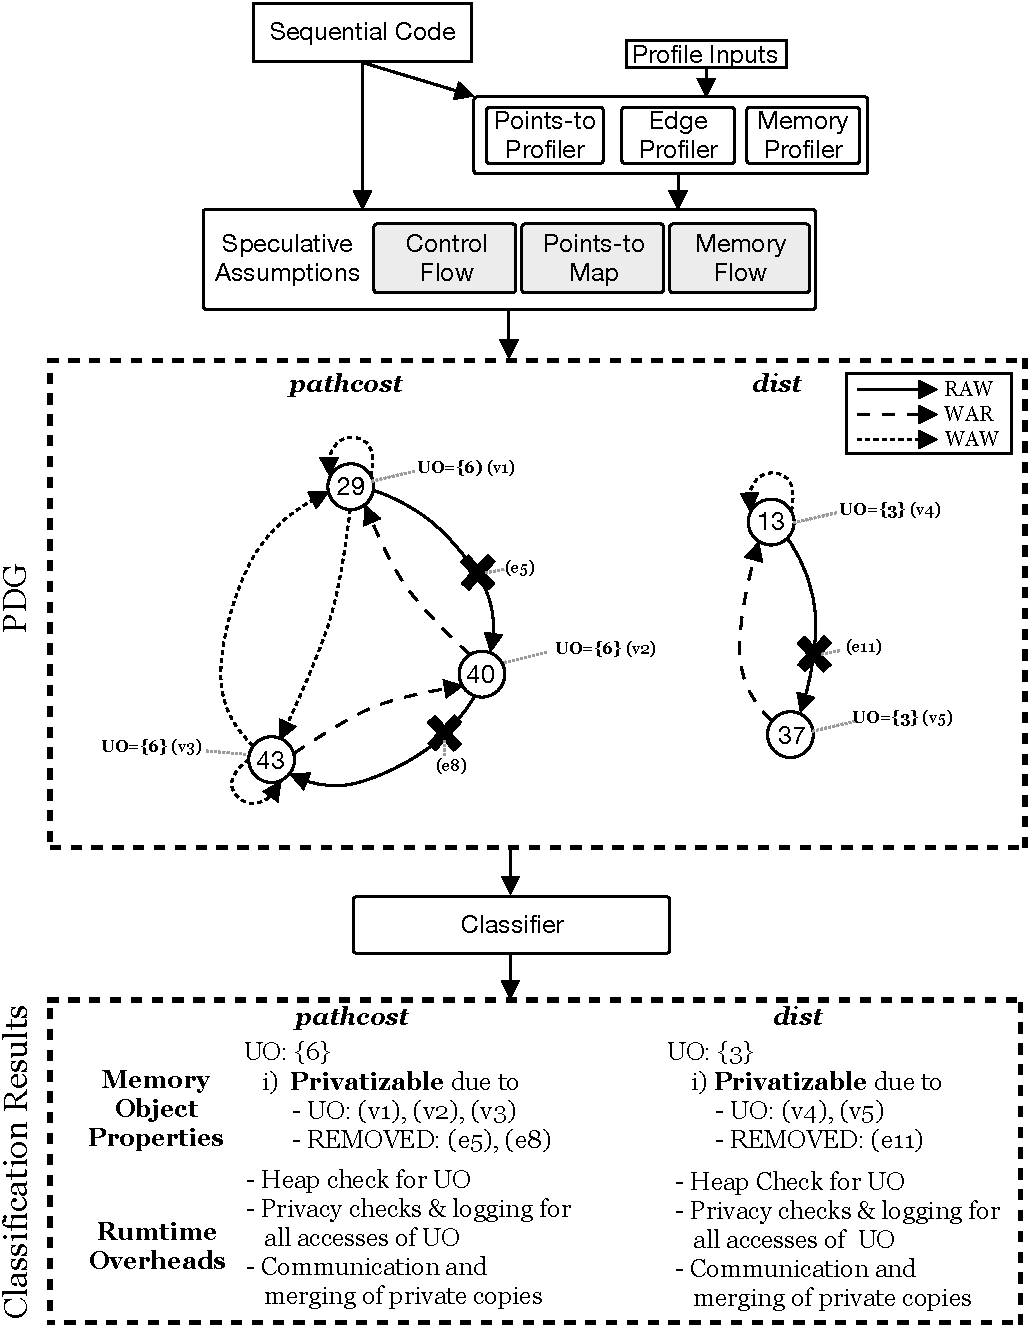
\includegraphics[width=0.46\textwidth]{figures/privateer-example-crop}
}
\qquad
\subfloat[\name (This Work)]{
  \centering
  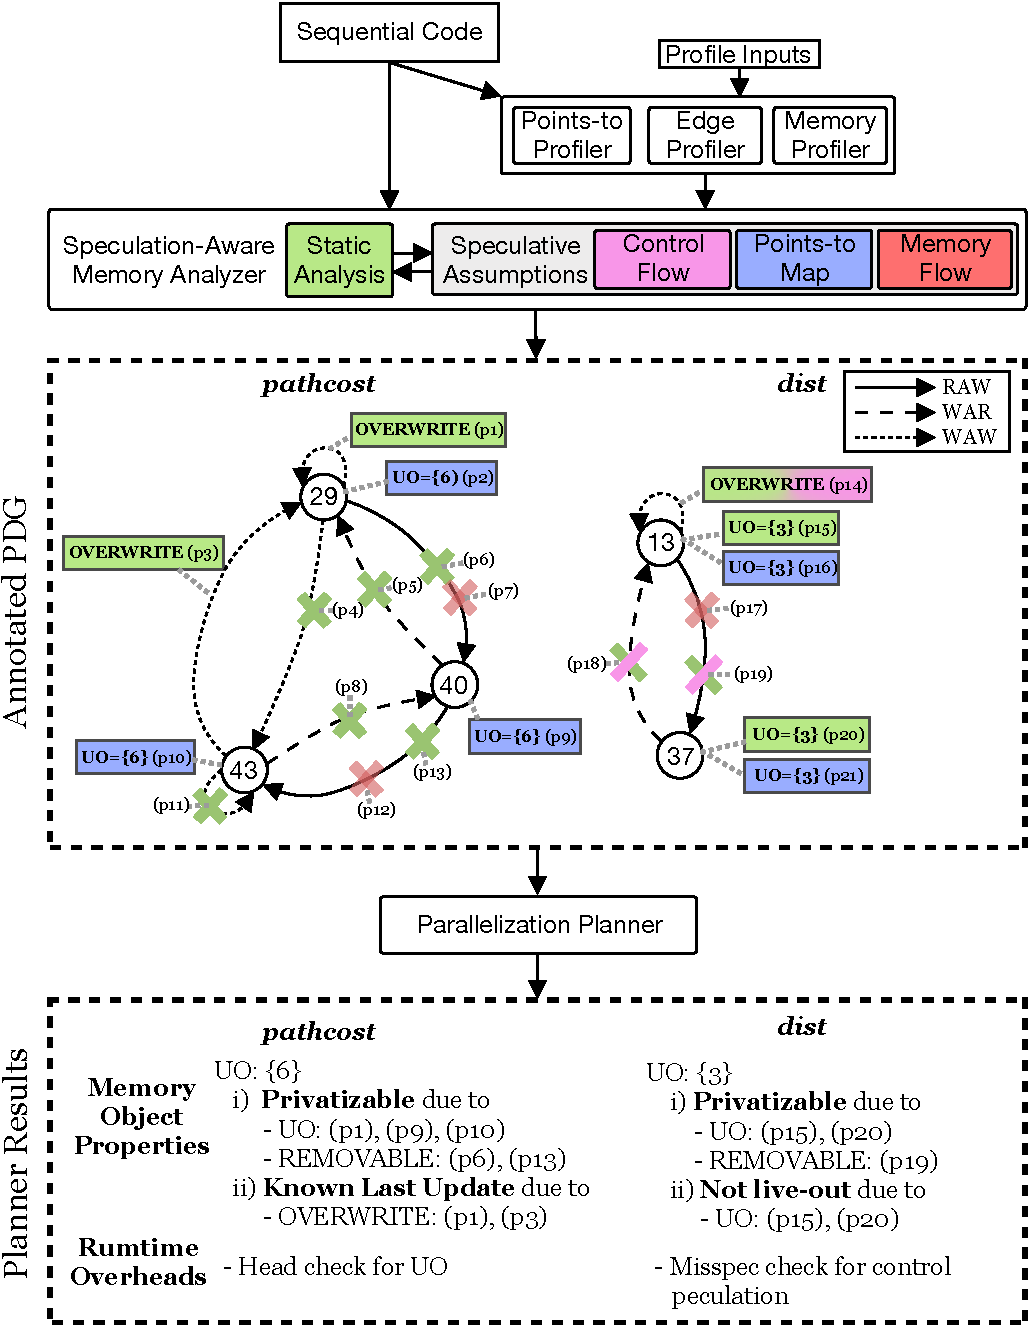
\includegraphics[width=0.46\textwidth]{figures/perspective-example-crop}
}
}
\caption{Comparison of decision process for handling memory
objects \texttt{\textbf{pathcost}} and \texttt{\textbf{dist}} of
\texttt{dijkstra}. Numbers in circles are line numbers in
Figure~\ref{fig:dijkstra_motivation}; ``UO=\{\#\}'' means the underlying
object is allocated/declared in line \#.}
\label{fig:dijkstra_motivation_comparison}
\end{figure*}

\begin{figure*}[!h]
\centering
\scriptsize
\resizebox{0.86\linewidth}{!}{
  % \subfloat[Sequential code]{
  %   \begin{minipage}{6cm}
  %     \begin{lstlisting}[morekeywords={pathcost,dist}, aboveskip=0pt, belowskip=0pt, firstnumber=1]
int *pathcost; // dyn alloc 1-D N
int *adj; // dyn alloc 2-D NxN
int dist;
int nDist;

void allocatePathCost() {
  pathcost = (int*)malloc(N*sizeof(int));
}

int dequeue() {
  if (!emptyQ()) {
\end{lstlisting}

\begin{lstlisting}[morekeywords={pathcost,dist}, aboveskip=0pt, belowskip=0pt,
firstnumber=13, name=dij_checks]
    dist = ...
    ...
  }
\end{lstlisting}

\begin{lstlisting}[morekeywords={pathcost,dist}, aboveskip=0pt, belowskip=0pt,
firstnumber=18, name=dij_checks]
}

void hot_loop(int N) {
\end{lstlisting}
\begin{lstlisting}[morekeywords={pathcost}, aboveskip=0pt, belowskip=0pt,
firstnumber=25]
  for (src=0; src<N; src++) {
\end{lstlisting}
\begin{lstlisting}[morekeywords={pathcost,dist}, aboveskip=0pt, belowskip=0pt,
firstnumber=28]
    for (i=0; i<N; i++)
      pathcost[i] = inf;

    enqueue(src, 0);
    while (!emptyQ()) {
      int v = dequeue();
      for (i=0; i<N; i++) {
\end{lstlisting}
\begin{lstlisting}[morekeywords={pathcost,dist}, aboveskip=0pt,
belowskip=0pt, firstnumber=38,name=dij_checks]
        nDist = adj[v][i] + dist;
\end{lstlisting}
\begin{lstlisting}[morekeywords={pathcost}, aboveskip=0pt, belowskip=0pt,
firstnumber=41]
        if (pathcost[i] > nDist) {
\end{lstlisting}
\begin{lstlisting}[morekeywords={pathcost}, aboveskip=0pt, belowskip=0pt,
firstnumber=44]
          pathcost[i] = nDist;
          enqueue(i, nDist);
        }
      }
    }
\end{lstlisting}
\begin{lstlisting}[morekeywords={pathcost}, aboveskip=0pt,
belowskip=0pt, firstnumber=52]
  }
\end{lstlisting}
\begin{lstlisting}[morekeywords={pathcost}, aboveskip=0pt,
belowskip=0pt, firstnumber=54]
}
\end{lstlisting}

  %   \end{minipage}
  %   }
\subfloat[Privateer~\cite{johnson:12:pldi}]{
  \centering
  \begin{minipage}{9.4cm}
  \begin{lstlisting}[morekeywords={pathcost}, belowskip=0pt, firstnumber=1,
name=dij_checks]
int *pathcost; // dyn alloc 1-D N
int *adj; // dyn alloc 2-D NxN
int dist, v, src, i;

for (src=0; src<N; src++) {
\end{lstlisting}

\begin{lstlisting}[morekeywords={pathcost}, aboveskip=0pt,belowskip=0pt,backgroundcolor=\color{lightgray},
firstnumber=auto, name=dij_checks]
  // Privacy Check
  private_write(pathcost, N*sizeof(int));
\end{lstlisting}

\begin{lstlisting}[morekeywords={pathcost},aboveskip=0pt, belowskip=0pt, firstnumber=auto,name=dij_checks]
  for (i=0; i<N; i++)
    pathcost[i] = inf;

  enqueue(src, 0);
  while (!emptyQ()) {
    dequeue(&v, &dist);
    for (i=0; i<N; i++) {
      nDist = adj[v][i] + dist;
\end{lstlisting}

\begin{lstlisting}[morekeywords={pathcost}, aboveskip=0pt,belowskip=0pt,backgroundcolor=\color{lightgray},
firstnumber=auto, name=dij_checks]
      // Privacy Check
      private_read(pathcost, sizeof(int));
\end{lstlisting}


\begin{lstlisting}[morekeywords={pathcost}, aboveskip=0pt, belowskip=0pt, firstnumber=auto,name=dij_checks]
      if (pathcost[i] > nDist) {
\end{lstlisting}

\begin{lstlisting}[morekeywords={pathcost}, aboveskip=0pt,belowskip=0pt,backgroundcolor=\color{lightgray},
firstnumber=auto, name=dij_checks]
        // Privacy Check
        private_write(pathcost, sizeof(int));
\end{lstlisting}

\begin{lstlisting}[morekeywords={pathcost}, aboveskip=0pt, belowskip=0pt, firstnumber=auto,name=dij_checks]
        pathcost[i] = nDist;
        enqueue(i, nDist);
      }
    }
  }
}
\end{lstlisting}

  \end{minipage}
}
\qquad
\qquad
\subfloat[\name (This Work)]{
  \centering
  \begin{minipage}{8.2cm}
  %\begin{lstlisting}[morekeywords={pathcost}, belowskip=0pt, firstnumber=1,
%name=dij_checks]
%int *pathcost; // dyn alloc 1-D N
%int *adj; // dyn alloc 2-D NxN
%int dist, v, src, i;


\begin{lstlisting}[morekeywords={pathcost,dist}, belowskip=0pt,
firstnumber=10, name=dij_checks, showlines=true]
int dequeue() {
  if (!emptyQ()) {


\end{lstlisting}

\begin{lstlisting}[morekeywords={pathcost,dist}, aboveskip=0pt, belowskip=0pt,
firstnumber=13, name=dij_checks]
    dist = ...
    ...
  }
\end{lstlisting}

  \begin{lstlisting}[morekeywords={pathcost}, aboveskip=0pt,belowskip=0pt,backgroundcolor=\color{lightgray}, firstnumber=auto, name=dij_checks]
  else // 0% added overhead
    misspec("Control misspec in dequeue()");
\end{lstlisting}

\begin{lstlisting}[morekeywords={pathcost,dist}, aboveskip=0pt, belowskip=0pt,
firstnumber=auto, name=dij_checks,showlines=true]
}

void worker_loop(int start, int N, int step) {

\end{lstlisting}

  \begin{lstlisting}[morekeywords={pathcost}, aboveskip=0pt,belowskip=0pt,backgroundcolor=\color{lightgray},
  firstnumber=auto, name=dij_checks,showlines=true]
  // Separation Local Check -- < 0.001% added overhead
  check_heap(pathcost, OVERWRITE_PRIVATE);
  \end{lstlisting}

\begin{lstlisting}[morekeywords={pathcost}, aboveskip=0pt,
belowskip=0pt, firstnumber=24,name=dij_checks,showlines=true]

  for (src=start; src<N; src+=step) {


\end{lstlisting}
\begin{lstlisting}[morekeywords={pathcost,dist}, aboveskip=0pt,
belowskip=0pt, firstnumber=28,name=dij_checks,showlines=true]
    for (i=0; i<N; i++)
      pathcost[i] = inf;

    enqueue(src, 0);
    while (!emptyQ()) {
      int v = dequeue();
      for (i=0; i<N; i++) {
\end{lstlisting}
\begin{lstlisting}[morekeywords={pathcost,dist,nDist}, aboveskip=0pt,
belowskip=0pt, firstnumber=auto,name=dij_checks,showlines=true]



        nDist = adj[v][i] + dist;
\end{lstlisting}
\begin{lstlisting}[morekeywords={pathcost}, aboveskip=0pt,
belowskip=0pt, firstnumber=auto,name=dij_checks,showlines=true]


        if (pathcost[i] > nDist) {


\end{lstlisting}
\begin{lstlisting}[morekeywords={pathcost}, aboveskip=0pt,
belowskip=0pt, firstnumber=auto,name=dij_checks]
          pathcost[i] = nDist;
          enqueue(i, nDist);
        }
      }
    }
\end{lstlisting}

\begin{lstlisting}[morekeywords={pathcost,dist}, aboveskip=0pt,
belowskip=0pt, firstnumber=auto,name=dij_checks,showlines=true]
  }
\end{lstlisting}

\begin{lstlisting}[morekeywords={pathcost},
aboveskip=0pt,belowskip=0pt,backgroundcolor=\color{lightgray},
firstnumber=auto, name=dij_checks,showlines=true]
  // only last iter's pathcost array
  // needs to be communicated -- < 1% added overhead
  if (src == N-1+step)
    communicate_pathcost();
\end{lstlisting}

\begin{lstlisting}[morekeywords={pathcost}, aboveskip=0pt,
belowskip=0pt, firstnumber=auto,name=dij_checks]
}
\end{lstlisting}

  \end{minipage}
}
}
\caption{Comparison of parallelized code of \texttt{dijkstra}. Logging and
checks during loop execution dominate the overheads, indicated in the code
as ``added OH''.}
\label{fig:dijkstra_motivation_comparison_source_code}
\end{figure*}
%caption,
%Checkpointing occurs every several (long running) loop iterations, thus its
%overhead is negligeable for \textit{dijkstra}.


\subsection{Example}
\label{motiv_example}

Next we describe how \name succeeds at parallelizing
\texttt{dijkstra} efficiently. This section also highlights the limitations
of prior work that blocked them as well as how the new concepts introduced
in \name overcomes them.
%
Consider again the code in Figure~\ref{fig:dijkstra_motivation},
briefly discussed in~\ref{motiv_overheads}.
%
Figure~\ref{fig:dijkstra_motivation_comparison} compares the
compilation flow of \name with that of Privateer for handling memory objects
\texttt{\textbf{pathcost}} and \texttt{\textbf{dist}}.

\name employs an exploration phase that yields a much more profitable plan
than Privateer's scheme.
%The PDG is annotated by the speculation-aware memory
Notice how the PDG is annotated with properties and underlying speculative
assumptions by the speculation-aware memory analyzer. Speculation-aware
memory analyzer allows removal of the RAW dependence between instruction
\textbf{13}
and \textbf{37} with a combination of static analysis and control speculation. This
dependence would require usage of memory speculation in prior work.
%
% Just removing dependences in the PDG creates ambiguity on how a
% dependence can be resolved, leading to over-speculation. The PDG
% contains useful properties even for non-removable dependences. For
% example,

Non-removable WAW edges in this example are annotated with
the \textit{overwrite} property that indicates that the destination
operation always overwrites the footprint of the source operation.
%
Based on the information on the PDG, three different transforms offer
handling of memory objects, including \textbf{overwrite privatization} and
\textbf{local privatization} proposed in
section~\ref{sec:enablers}.

%For example, handling of \textit{dist} requires usage of control
%speculation (for the branch in line 11,
%fig.~\ref{fig:dijkstra_motivation}).
%
%Notice that \textit{dist} can be handled by all three
%transformations.
%
The DOALL planner then selects the lowest cost solution for each memory
object. For example, the local privatization's
offer is selected for \texttt{\textbf{dist}} since it is the cheapest
privatization transform and its
speculative assumption is the same as those of other options'.
The \texttt{\textbf{nDist}} object (not shown in this figure) is also handled
by local privatization. \texttt{\textbf{pathcost}} is resolved by overwrite
privatization.
% %
% Extracting this efficient plan would not be possible without the use
% speculation-aware memory analyzer and efficient speculative
% privatization transformations.

% From prior work, Privateer~\cite{johnson:12:pldi} is the only
% automatic system to support privatization of dynamically allocated
% objects, like \textit{pathcost}, even in the presence of unrestricted
% pointers.


%
Privateer, on the other hand, without the support of speculation-aware
memory analyzer and  efficient speculative privatization transform, relies
on profile information to infer that these two objects are privatizable and
is forced to apply transforms with privacy checks and merging of private
copies, resulting in high runtime overheads. The use of the relaxed PDG,
whose dependences are removed a priori with speculation, necessitates
instrumenting checks, as it is ambiguous how each dependence was removed.
Moreover, this prevents the more efficient variants of privatization to be
used because static analysis cannot infer post priori the properties of an
object without knowing its speculative assumptions.

%Even if memory analysis was used instead of memory speculation, the
%classifier sees the optimistic view of the program
%


%not only in Privateer but in any other automatic parallelization
%speculative system.


%Whilst the private property is enough for DOALL
%Notice that we infer an additional property that improves the profitability
%of parallelization.

%For inferring the property that a private memory object has the additional local-private
%property, it suffices to identify all accesses of the memory object
%and check that all of them are within the loop.
%locally-accessed property.


Figure~\ref{fig:dijkstra_motivation_comparison_source_code} compares the
resulting parallelized versions (in a simplified form) of \name and
Privateer. The code includes all the added checks, logging, and live-out
handling overheads. The code changes are marked with the average added
overhead compared to the useful work of each worker. It is clear that \name is
able to parallelize \texttt{dijkstra} with minimum overheads thanks to the
use of speculative-aware memory analyzer, careful selection of applied
transformations, and use of efficient privatization variants. In fact,
\name exhibits 4.8$\times$ speedup over Privateer for \texttt{dijkstra}
(see~\ref{eval}).

%Privateer would choose to just do simple privatization with mem spec.
%The spec-aware analyzer allows removal of mem spec and efficient
%privatization in this case.
%
%\begin{itemize}
%\item
%Privatization of these memory objects requires:
%\begin{enumerate}
%\item
%identification of all accesses of these objects
%    within the loop
%\item
%absence of cross-iteration flow
%     dependences on each of these accesses
%\end{enumerate}
%
%\end{itemize}
%
%
%DOALL can become applicable if these two objects are proven to have the
%private property.
%
%We compare our approach where we combine static analysis with cheap-to-validate
%with privateer's monolithic approach that over-speculates and is limited by high
%runtime overheads.
%
%Note that anti-dependences are ignored since both systems use
%process-based runtime systems.

 %\section{Framework Overview}

\begin{figure}[htp]
  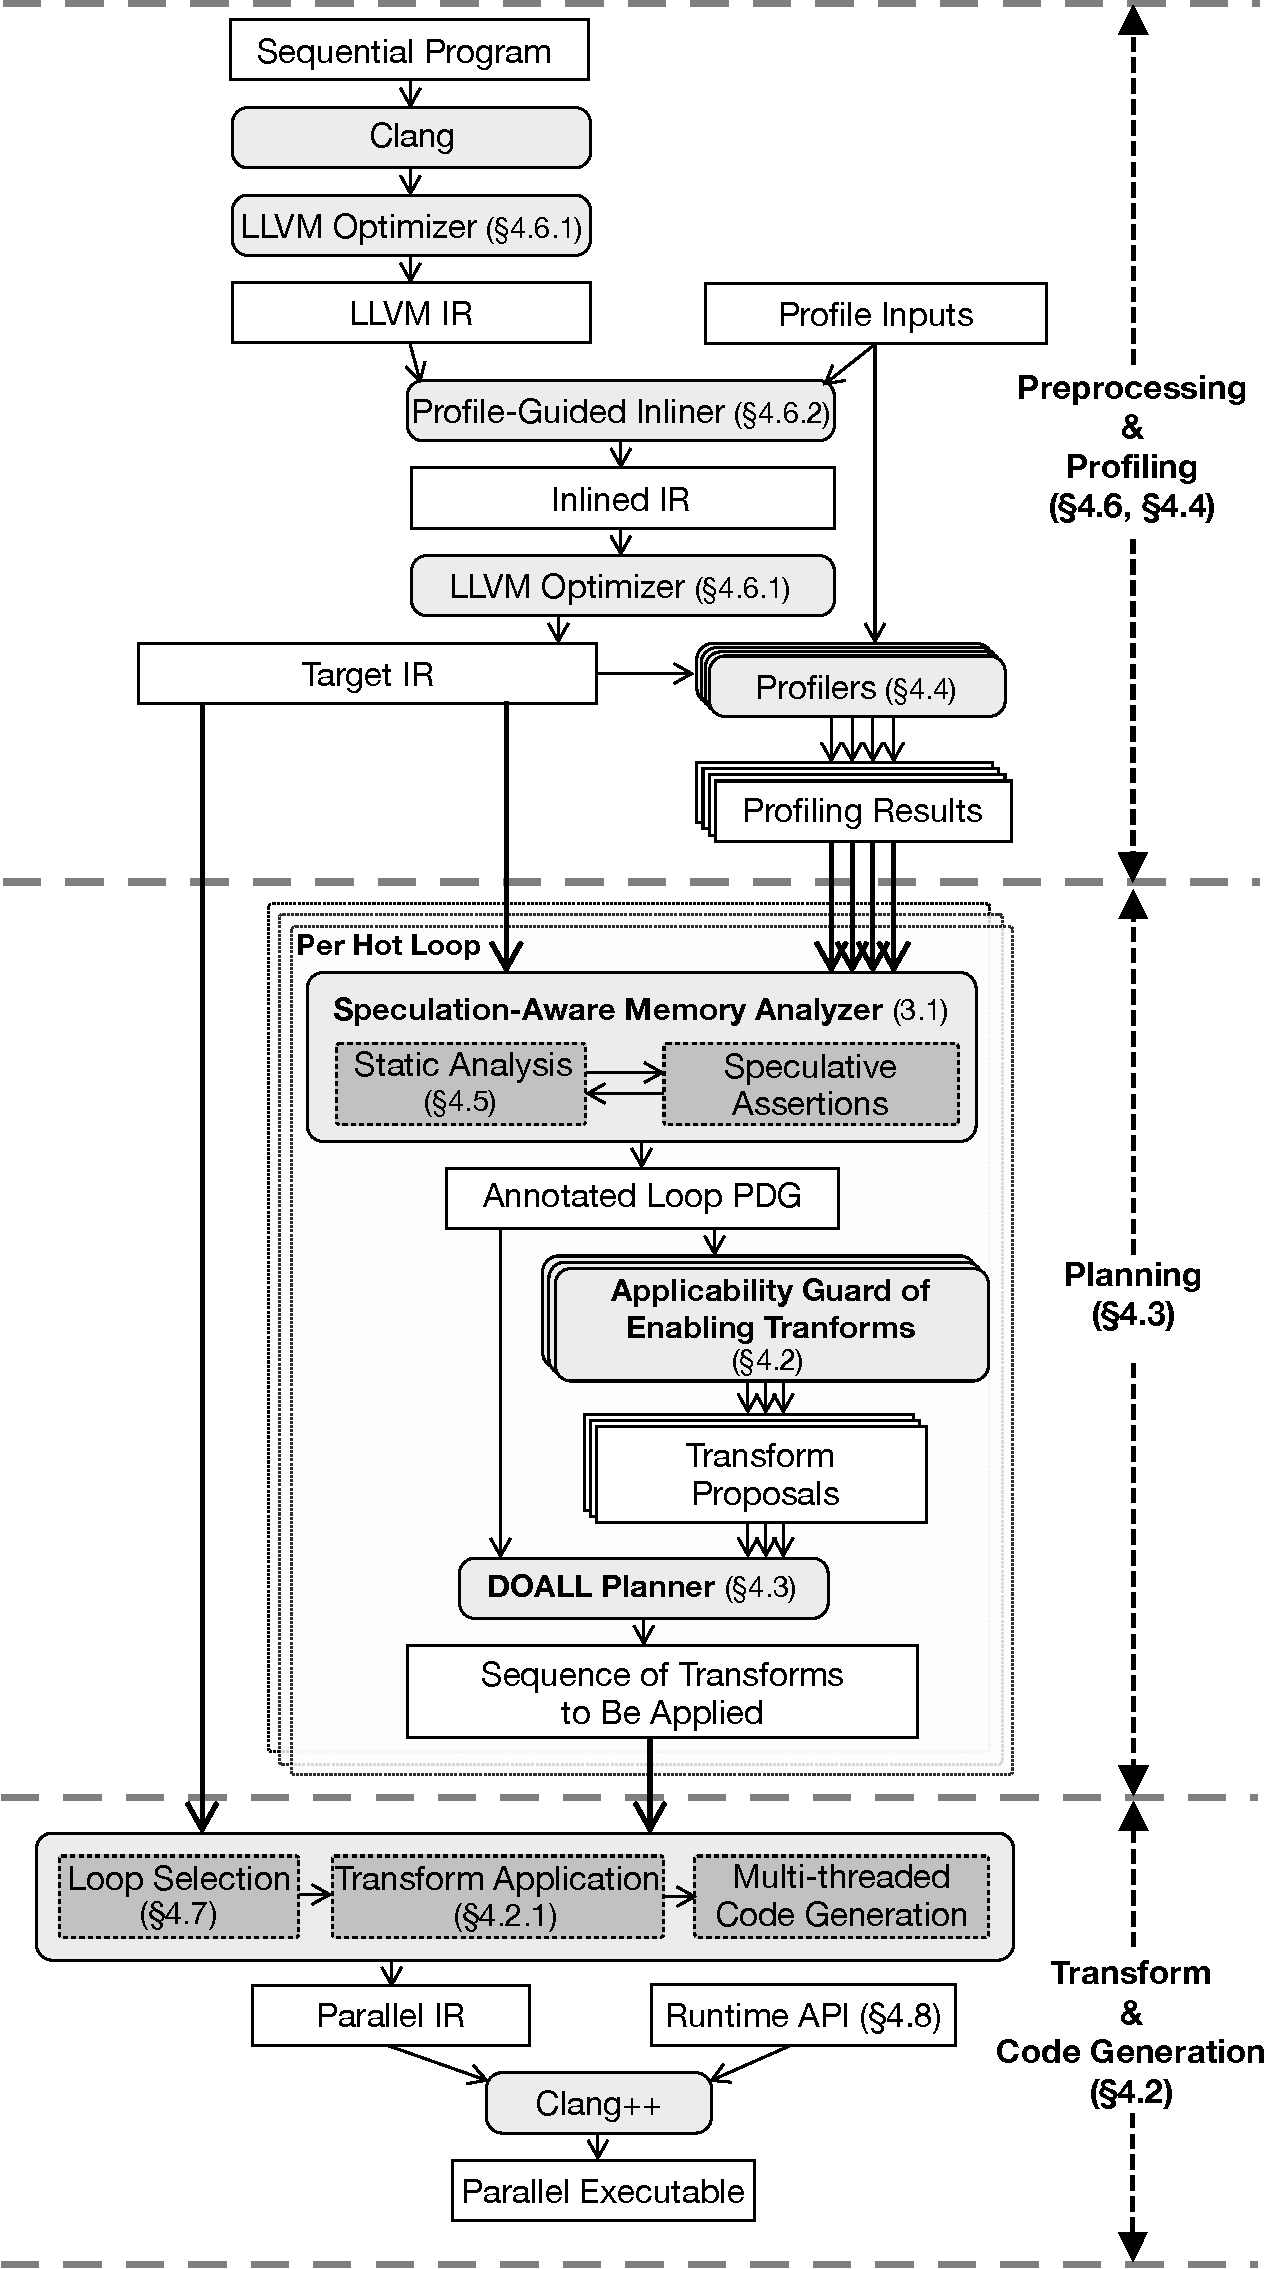
\includegraphics[width=\columnwidth]{figures/compiler-pipeline-crop}
  \caption{Framework Overview}
  \label{fig:compiler-pipeline}
\end{figure}

LSD enables efficient speculative parallelization by leveraging fine-grained
combination of static analysis and cheap-to-validate assumptions.
%
Figure~\ref{fig:compiler-pipeline} depicts an overview of the LSD system, which
includes a set of profilers, a parallelizing compiler and a runtime system.
%
The compiler can be split into three regions: Analysis, Planning, Transformation
and Codegen.

We have implemented LSD within the LLVM infrastracture. Fig.
\ref{fig:compiler-pipeline} presents the compiler pipeline of our framework. As
the first step, the sequential program is complied, inlined, and optimized into
a target LLVM intermediate representation (IR) which is then used to generate
profiling results. In the second phase, we focus on each hot loop, leveraging
static and speculative analysis to generate a PDG annotated with properties of
dependences. The analyses for transformations then examine every remaining
loop-carried dependences and propose plans to remove them. A DOALL planner
considers these proposals and generate a sequence of transformations if a
profitable DOALL plan is available. Finally, we select a set of compatible loops
with the maximum profit, apply tranformations, and generate the parallel IR
which is linked with an efficient uniqued runtime and compiled as the
parallel executable.

 \section{Framework Design and Implementation}

\begin{figure}[htp]
  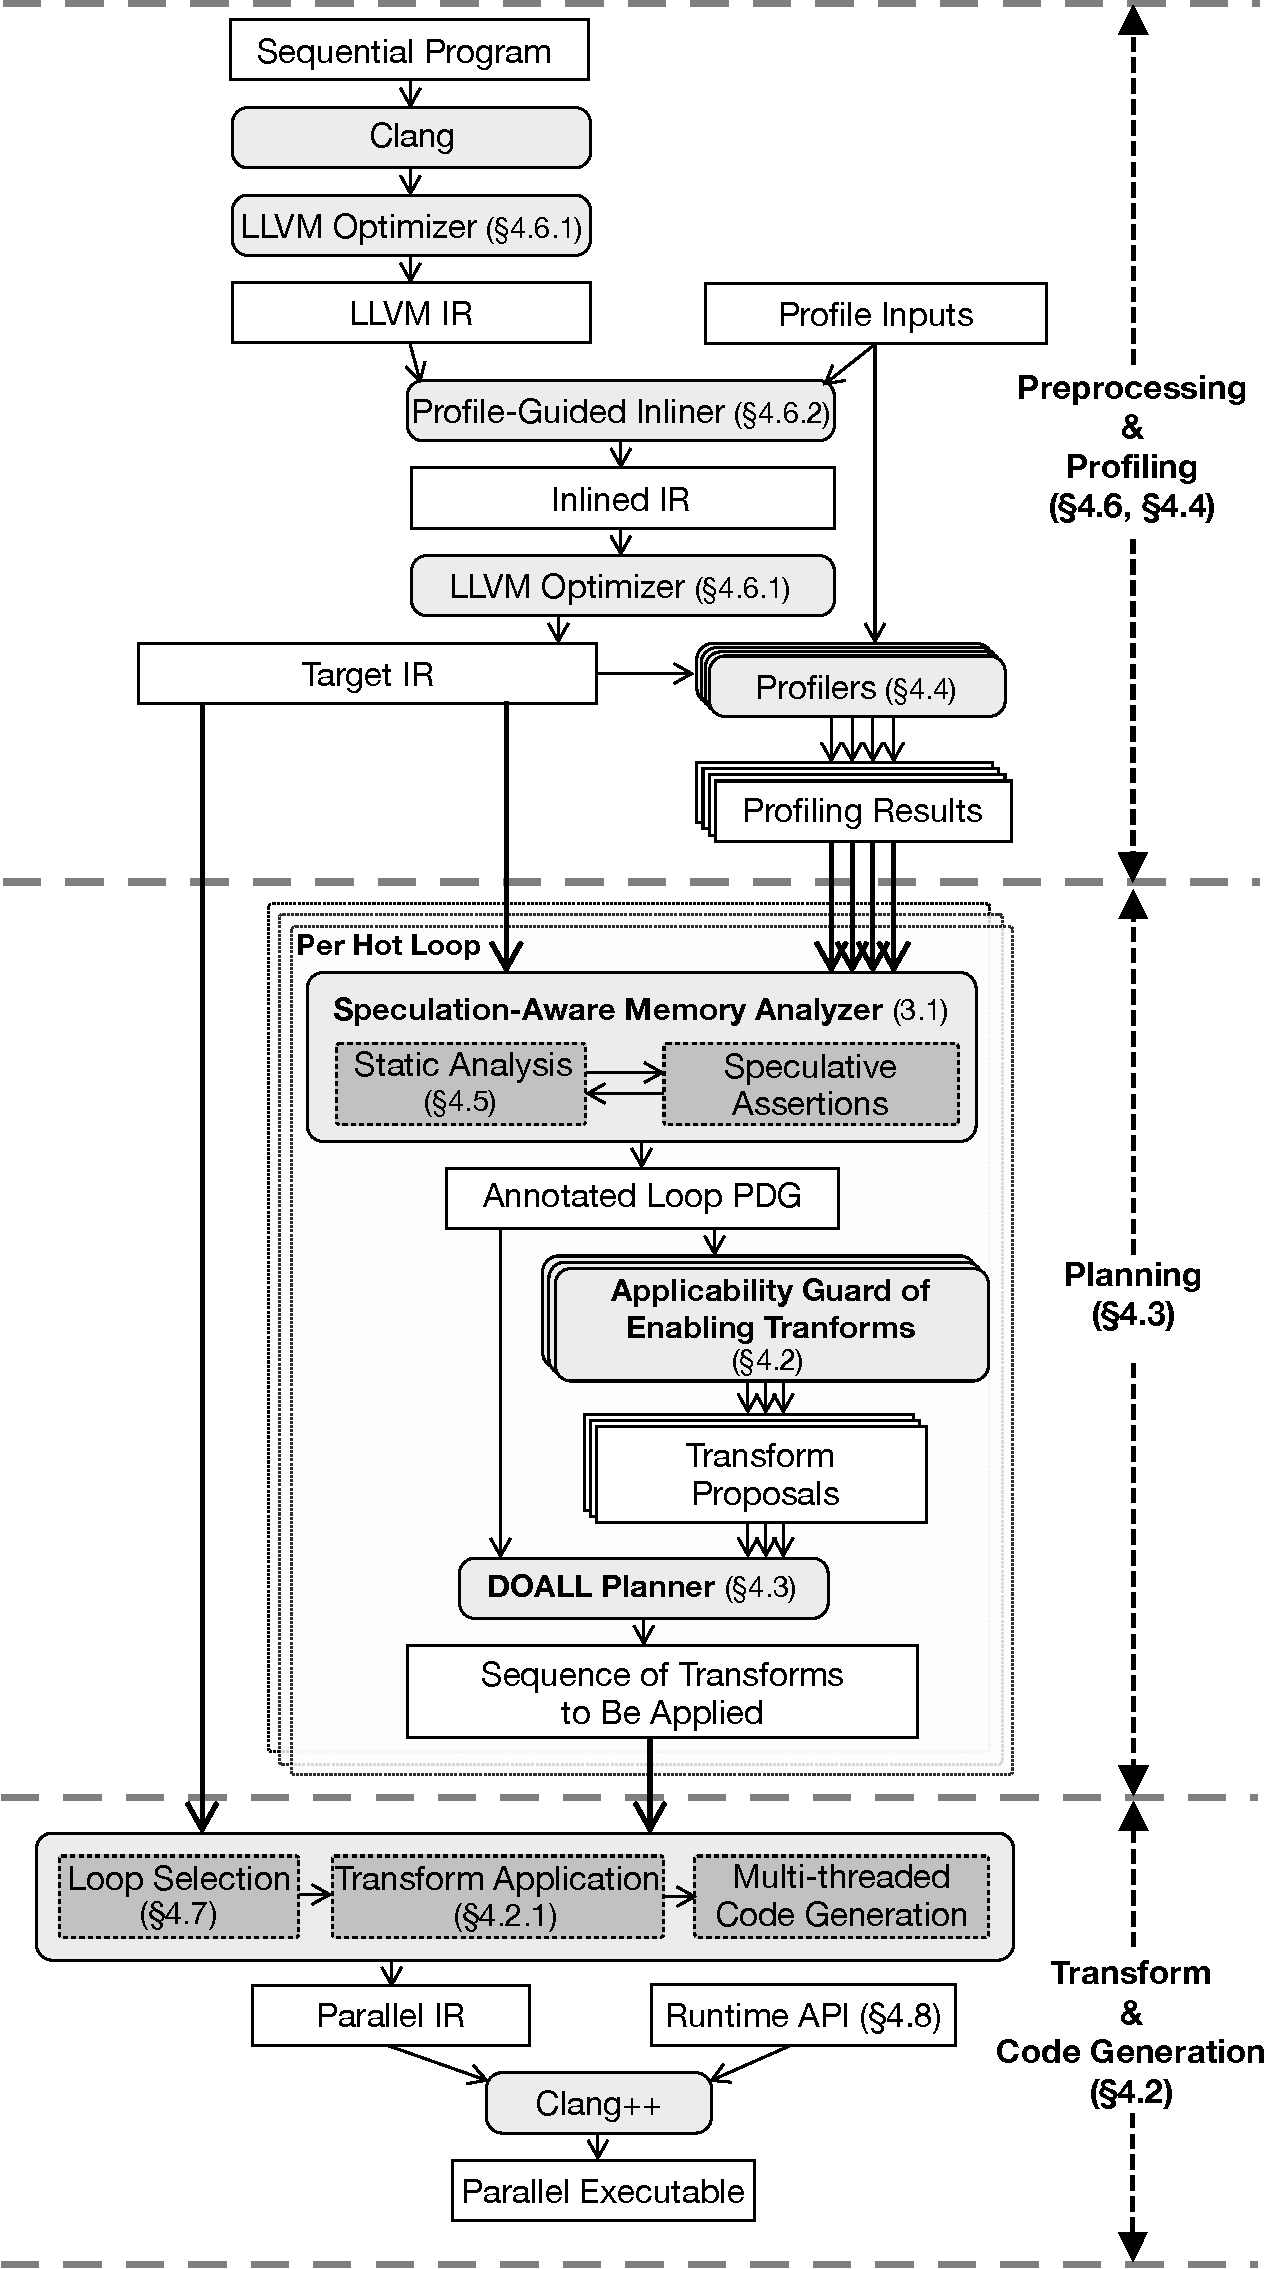
\includegraphics[width=\columnwidth]{figures/compiler-pipeline-crop}
  \caption{\name Framework Overview}
  \label{fig:compiler-pipeline}
\end{figure}

%\name enables efficient speculative parallelization by leveraging
%fine-grained combination of static analysis and cheap-to-validate
%assumptions.
%
\name is a framework for DOALL parallelization that incorporates the
ideas described in section~\ref{sec:approach}.


Figure~\ref{fig:compiler-pipeline} depicts an overview of the \name
framework, which includes a set of profilers, a parallelizing compiler,
and a runtime system.
%
The compilation flow begins with a preprocessing step that adds
instrumentation in the LLVM intermediate representation (IR) for
generating profiling results, from which a set of hot
loops is selected.
% In the second phase of the compilation, each hot
% loop is processed separately.
The speculation-aware memory analyzer
is queried to annotate the PDG with properties regarding dependences and
instructions. The applicability guard of each enabling
transformation examines the annotated PDG and creates transformation
proposals that offer to remove parallelization-inhibiting cross-iteration
dependences in the loop along with its cost. A DOALL planner considers
these proposals, selects set of minimum cost options and generates a sequence
of transformations, if a profitable DOALL plan is available.
Finally, we select a set of
compatible parallelizable loops with the maximum profitability, apply the
tranformations in their plans, and generate the parallel IR which is
then linked with the runtime and compiled as the parallel executable.

 This section begins with discussion of the planning phase which
 includes the main contributions of this paper and then subsequently
 describes other components of the framework.

\subsection{Speculation-Aware Memory Analyzer}
\label{sama}

%
% Prior techniques independently apply speculative techniques to
% overcome the imprecision of memory analysis, often leading to
% excessive use of expensive memory speculation.
%
%This work suggests that exposing cheap-to-validate speculative
%assumptions to static analysis can enable removal of memory
%dependences that would otherwise require memory speculation.
%
%This combination yields higher precision than using static analysis
%and these assumptions in a sequence.
%
%By making memory analysis aware of cheap-to-validate speculative
%assumptions,
%
This work proposes a speculation-aware memory analyzer that
combines the strengths of static analysis and cheap-to-validate
speculative assumptions to reduce the need for expensive speculation by
interpreting cheap-to-validate speculative assumptions as facts when memory
analysis fails.
%
The inclusion of speculation changes the semantics of traditional
memory analysis. It is now required to specify for each answer the
speculative assumptions, if any, that were used in the process.
%
This differs from applying speculation and querying memory analysis again
since the possibility of misspeculation restrains static analysis.

%When a query is received the memory analyzer tries to resolve it with
%usage of just static analysis. If that fails, it tries to use memory
%analysis with cheap-speculative assumptions.
%If that still fails then it resorts to memory speculation.
%
%
%Memory analysis annotates a PDG with information utilized by the
%decision making process in the rest of the planning phase.

\name's memory analysis is composed of many simple analysis algorithms
that collaboratively respond to queries (e.g.
CAF~\cite{johnson:cgo:17}).
%
The modularity of our static analysis simplifies the addition of
speculation awareness. Only the analysis algorithms that could
benefit from the collaboration need to be extended with a
speculative mode.
%
% A monolithic memory analysis would be harder to extend for speculation
% awareness.

In the speculation-aware memory analyzer, \name utilizes speculative
assumptions from two profilers: edge profiler (detects biased
branches) and loaded value predictor (predicts loaded values).
%
While use of these two speculative assumptions in conjuction with
static analysis already enables up to 2.5$\times$ improvement over a
system with no collaboration of memory analysis and speculation (see
~\cref{eval}), exposing even more cheap-to-validate speculative
assumptions to memory analysis could also be beneficial.  Such
exploration is left for future work.
%This paper just stratches the surface of this

\name uses edge profiling to produce a speculative control flow. This
speculative control flow can be used by memory analysis passes to
handle more queries.
%
Two examples of analysis passes that benefit from this speculative
information is kill-flow and unique access paths (UAP) algorithms.
%
Kill-flow analysis disproves memory dependences by finding killing
operations along all feasible paths between two operations.  If
kill-flow uses speculative control flow information, the feasible
paths are reduced and kill-flow asserts absence of a statically
non-disprovable memory dependence.
%
UAP collects a points-to set of objects for a pointer stored into a
non-captured memory location (i.e., address never stored into memory
and never passed to an externally defined function).
%Alias queries related to this memory location produce new alias
%queries for each value stored in this memory location.
Use of speculative control flow information enables detection of
speculatively dead stores in this set, decreasing its size and thus
simplifying alias queries for this pointer.

%In both examples, without speculative control flow awareness, prior
%speculative parallelization systems would be forced to use expensive
%memory speculation instead.

Regarding value prediction, if memory analysis passes assume that
loaded value predictions are correct, then they can re-interpret a
predicted load as a store of the predicted value. One analysis
algorithm that can benefit from that is again kill-flow. Kill-flow
treats the predictable load as a kill operation for must-aliasing data
flows.

%Apart from removal of dependences, the speculation-aware memory
%analyzer is also used to characterize dependences.
%%and dependent instructions.
%%
%Traditionally, dependence analysis (static, dynamic or speculative) in
%speculative parallelization only attempts to completely remove
%dependences.
%%
%If a dependence cannot be removed even with usage of speculation,
%because it is a real dependence that frequently manifests at runtime,
%no useful information is provided related to this dependence.
%%
%The memory analyzer though could still infer some useful property for
%this dependence or the dependent instructions.
%%
%This information is essential to enable certain transformations, such
%as the efficient variants of speculative privatization described in
%section ~\ref{novel_transf}.

The speculation-aware memory analyzer is queried to populate a program
dependence graph (PDG) annotated with information utilized by the rest
of the planning phase, namely by enabling transformations and the
planner. Annotations include properties for the dependences and the
dependent instructions.
%Note that traditional dependence analysis (static, dynamic or
%speculative) in speculative parallelization only attempts to
%completely remove dependences, while the speculation-aware memory
%analyzer infers properties for even non-removable ones.
If a property cannot be statically inferred, then annotations may
include alternatives; decision making is left for the planner.
%, which can perform global reasoning.
%The planner is responsible for selecting the most profitable option,
%taking into consideration. Memory analyzer has a limited scope.


\subsection{Enabling Transformations}
\label{enablers}

% Transformations modify the code to remove parallelization inhibitors.
%
All transformations in \name are split into two parts: (1) the applicability guard
that participates in the planning phase of the compilation, and (2) the
actual transformation that, if selected, is applied in the
transformation phase.
%This scheme seperates the desicion part from the actual
%transformation and allows us to evaluate the cost of each dependence
%separetely and
% This separation of decision making and application of transformations
This allows careful selection the most profitable plan instead of
applying a fixed
% (regardless of the input program)
set of enabling transformations and speculative techniques.

%Enabling transformations address memory, register or/and control
%cross-iteration dependences.
%
% This section focuses on memory related enabling transformations.
% Register and control cross-iteration dependence handling is discussed
% in section~\ref{design_transf}.

% \subsubsection*{Memory-related Enablers}

% To enable DOALL parallelization all cross-iteration memory dependences
% need to be addressed.  However, many enabling transformations operate
% at a memory object level. For example, the privatization
% transformation create private copies of memory objects. This motivates
% an object-centric approach.  Instead of targeting cross-iteration
% dependences, enabling transformation offer to handle a set of memory
% objects, in effect offer to address all their cross-iteration
% dependences.

%Characterizing the behavior of memory objects requires
%%(i) identification of accesses to this object within the loop and
%(i) mapping memory accesses to objects and (ii) analysis of the
%dependences that these accesses introduce.
%% characterize accesses
%This work attempts to satisfy these two requirements by using a
%combination of cheap-to-validate speculative assumptions and static
%analysis.
%
%The \textit{applicability} guard of an enabling transformation
%determines which memory objects have certain properties required by
%the transformation.
%
%examines the memory objects in the loop's memory footprint and
%determines which memory objects
%
%The applicability guard of a transformation determines, using the
%results of the speculation-aware memory analyzer,  which memory
%objects have certain properties required by the corresponding
%transformation and under which assumptions.
%%
%Assumptions are speculative information that require validation for
%the transformation to be correct, while applicability for a memory
%object means that the transformations can address all the
%cross-iteration dependences related to this memory object. \{\textbf{XXX}
%Pretty unclear what these two sentences means\}


%
\paragraph{Applicability:}
%
The applicability guard of a transformation uses the results of the
speculation-aware memory analyzer to determine which memory objects
satisfy the properties required by the transformation and records the
speculative assumptions used.
%
% XXX Make sure to add that assumptions need to be validated at runtime
% later on
% The applicability guard also records the speculative assumptions used
% to infer applicability for a memory object. These assumptions would
% need to be validated at runtime for the transformation to be correct.

\paragraph{Transformation proposal:} The output of each applicability
guard is assembled in a transformation proposal which is sent to the
DOALL planner (\cref{planner}).
%
The proposal includes for each memory object an estimated handling
cost based on the transformation itself and the validation cost of the
used speculative assumptions.
%
%The cost of each transformation is determined by the cost of the
%transformation itself and the cost of the speculative assumptions
%required for the transformation to be applicable.
%
For simplicity, each transformation and speculation
validation operation is assigned a fixed
%predefined
cost that ensures a basic ordering among the options. For
example,
%regarding speculative assumptions,
memory speculation has an extremely high cost (expensive validation),
loaded value prediction has a much smaller cost, while
control speculation has no cost.
%The estimated cost computation is very basic and just ensures basic
%ordering among the options.
%
%Every transformation is assigned an arbitrary cost that ensures some
%ordering among transformation. Speculative assumptions is similarly
%computed.
%
For the set of transformations and speculative assumptions in our
framework and in the context of DOALL parallelization, this simplified
cost model proved sufficient for detection of minimal cost plans.
%
%A more complex cost model, that would allow more elaborate decision
%making, is left for future work.

%
%
%which speculative assumptions need to be validated for the
%transformation to be correct.
%
%Object-centric transformation.  All memory objects need to be handled
%by a transformation.
%
%each access of the memory object should preserve the property
%
%Finally, each transformation
%includes in its proposal the set of speculative assumptions validation
%necessary for each memory object for the transformation applicability
%to be correct.

\paragraph{Transformation Application:}
Each transformation reallocates
memory objects it is selected to handle
%If, during the planning phase, a transformation is selected for a set
%of memory objects, then during the code transformation phase, the
%transformation separates these objects
to its own heap, disjoint from any others; transformations may also
perform additional transformation-specific modifications.

Separating the objects is essential
for two reasons. First, each transformation may demand different
memory mapping semantics and handles objects differently at commit.
Second, mapping of memory accesses to
objects often relies on profiling information, especially in languages with
unrestricted pointers like C/C++. Ensuring that all objects' accesses
are contained within a transformation's heap is sufficient to
validate underlying object assumptions. This idea of separation has
been explored previously by Johnson et al. (Privateer~\cite{johnson:12:pldi}).
The speculative assumptions used for each selected transformation also need
to be validated at runtime to ensure correctness.
% The applicability guard also records the speculative assumptions used
% to infer applicability for a memory object. These assumptions would
% need to be validated at runtime for the transformation to be correct.
%Separation checks are required for memory accesses whose underlying
%objects are discovered via profiling.
%The runtime function for re-allocation of memory objects can be
%specialized by each transformation.
%
%Each transformation has its own runtime support for handling its
%objects during execution.

%The idea of separating memory objects has been explored previously by
%Johnson et al. (Privateer~\cite{johnson:12:pldi}).  However, Privateer
%employs a monolithic design that entangles classification of memory
%objects with memory speculation and other
%%monolithic design of memory object classification entangles
%%separation speculation with memory speculation and other
%profiling-based information, resulting in unnecessarily high runtime
%overheads (see example in section~\ref{motiv_example} and performance
%analysis in section ~\ref{eval}).
%%
%By contrast, \name employs a modular and extensible design that
%facilitates planning and selection of minimal cost solutions without
%unnecessary speculation.
%where enabling transformations offer to handle memory objects along
%with estimated costs -offers with costs and the selection happens.
%

%Every transformation can optimize the checks that are applied to its
%objects knowing that there is no aliasing with other objects handled
%by different transformations.

%ensures that all accesses of a memory object have the required
%properties.

% We describe in the next section efficient variants of the speculative
% privatization transformation, which constitute a contribution of this
% paper.  Other enabling transformations that are used in our framework
% but have been proposed in prior work are discussed in
% section \ref{design_transf}.
We propose the following enabling transformations for addressing memory,
register, and/or control cross-iteration dependences.

Enabling transformations address memory, register or/and control
cross-iteration dependences.

\subsubsection{Memory Dependences}

Memory-related enabling transformation collect a set of memory objects
for which they are applicable (see ~\ref{enablers}).

%TODO: maybe add discussion about their cost

\begin{itemize}
%
\item Privatization: Discussed in ~\ref{novel_transf}

\item Reduction: Applicable for objects that only participate to
reduction operations. When applied, separates its objects to the
reduction heap and inserts separation checks (check that their
accesses are within this heap). During runtime, separation is checked
and at commit objects of parallel workers are
merged according to their reduction operation.

%Applicability guard: objects that only participate to reduction
%operations

%Transformation Application: only separate objects to reduction heap

%Runtime support: at commit merge all objects according to their
%reduction operation

\item Short-lived: Applicable for objects that only exist within one
iteration of the loop. When applied, separates its objects to the
short-lived heap and inserts check to ensure separation and that all
the objects of the heap are freed at the end of the iteration. During
runtime, the short-lived property and separation are checked.

\item Read-only: Applicable for objects that are never written to.
When applied, separates its objects to the read heap and inserts
separation checks.  During runtime, separation is checked.

\item TXIO: Applicable for shared IO objects. When applied, it
replaces IO library calls with custom calls. During runtime, it
collects output operations and performs them in order at commit.

\end{itemize}

\subsubsection{Register \& Control Dependences}

Cross-iteration register dependences
%(not related to induction variables)
are handled with reduction, replication, control speculation or value
prediction. Replication replicates side-effect free computation across
parallel workers to overcome cross-iteration dependences and avoid
inter-thread communication.
%
Cross-iteration control dependences are handled either with
replication or control speculation.
%mention IV?
Use of replication allows handling of uncounted loops, namely loops
with unknown trip count when the loop is invoked.
%
In terms of transformation cost, all transformations have constant
cost except for replication.  Replication's cost depends on how many
instructions need to be replicated. Non-speculative enablers
(reduction and replication) are preferred, in most cases, over
speculative ones, and reduction is preferred over replication.

%Cross-iteration register and control dependences related to induction
%variables are handled differently if detected.

%handling live-outs, loop-carried
%
%In the case of speculative executive, registers with cross-iteration
%dependences and live-out registers
%are stored in memory at commit so that they are recoverable in case of
%misspeculation. For live-outs, storing to memory

%\begin{itemize}
%
%\item Scalar Reduction
%
%\item Replication: Replicate side-effect free computation across
%parallel workers.
%
%\end{itemize}
%
%\subsubsection{Control Dependences}
%
%\item Induction Variable Detection: Every worker gets assigned a
%
%\item Replication: Replicate cross-iteration control dependences for
%each worker
%
%\item Control Speculation: Speculate cross-iteration control
%dependences


%\subsubsection{Efficient Speculative Privatization Variants}
\subsubsection{New Enablers}
\label{novel_transf}

%Ensuring correct live-out memory state often requires extensive bookkeeping,
%during parallel execution, for the write footprint of private objects. To make
%parallelization more \textit{profitable}, this work expresses more properties
%for private memory objects. Private objects could additionally (a) be
%independent~\cite{ARRAY_privatization} (no loop-carried false dependences); (b)
%have loop-invariant condition for last update within the
%loop~\cite{ARRAY_privatization}; (c) have predictable live-out content;
%%(not found in prior work);
%or (d) have only local accesses (allocated outside the loop, but all
%accesses are contained within the loop execution).
%%
%%Private properties (a), (b) have been explored before in the context of static
%%parallelization~\cite{ARRAY_privatization}, but never before in speculative
%%parallelization systems (maybe in LRPD). No prior work leveraged property (c).
%%
%

% We first discuss speculative privatization as it appears in prior work
% and then describe new variants that perform more efficient
% privatization.

% This section describes the behavior of the new enablers introduced in
% \cref{new_enablers}.
% Prior software speculative systems with extended support for
% privatization~\cite{johnson:12:pldi,kim:12:cgo} only infer the basic
% privatization property that there are no cross-iteration data flows
% for a memory object.
%
% Speculative privatization application involves instrumentation of all
% write accesses of privatized objects for costly logging or
% communication. At commit, the private copies of each worker are merged
% according to metadata that specify which worker wrote each byte last.

To avoid expensive monitoring of write sets during parallel execution
and minimize copy-out costs, we propose four efficient variants of
this transformation, introduced in \cref{new_enablers}. This section
describes the behaviors of each of them at runtime.
%
% To be applicable, these variants require apart from the basic
% privatization property additional memory object properties.

%Table~\ref{tab:priv_types} summarizes how these properties can facilitate more
%efficient parallelization compared to just inferring that a memory object is
%private. In short, inference of any of these four private properties allows
%complete elimination of bookkeeping and access checks. Prior software
%speculative systems with extended support of privatization (Privateer~\cite{},
%ClusterDoall~\cite{}) are only able to infer the simple private property and
%thus always require costly checks or monitoring.

\begin{itemize}
%
\item \textbf{Independent:} This transformation's heap is shared
  among all parallel workers, since there is no overlapping memory
  accesses.
  %
  No monitoring of write sets is needed. At commit the heap is copied-out
  to the non-speculative state.
%
%If the selected parallelization plan is non-speculative, then this
%heap is also shared with the main process and copy-in and copy-out
%overheads are eliminated as well.

%Behavior : No write set monitoring performed. Memory object is shared among parallel workers.

\item \textbf{Overwrite Private:} This transformation's heap has
  CoW (copy-on-write) mapping. At the end of the parallel
  invocation the last executed iteration
  state is copied-out and no monitoring is needed.

%Additional applicability guard:
%object has loop-invariant condition for last update within the loop.
%
%Behavior: No write set monitoring performed. The live-out state for
%object with this property is the memory state of the last iteration
%executed before commit.

\item \textbf{Predictable Private:} This transformation's heap
  has CoW mapping. The live-out state is predictable, so no monitoring
  or merging of parallel workers state is needed. This transformation
  relies on value prediction's speculative assumptions.

\item \textbf{Local Private:} This transformation's heap has
  CoW mapping and there is no need for copy-out or monitoring.

\end{itemize}

The first two variants have been explored by Tu et
al.~\cite{tu:94:lcbc} but were limited to static analysis
based detection of privatization. Unlike prior work, \name
extends applicability of these variants with usage of speculative
assumptions to programs with pointers, dynamic allocation, and type
casts.

%\centering
\tiny
\begin{tabular}{|c|c|c|c|c|c|c|c|c|}
  \hline
  Type of Private &
  Overlap         &
  Spec Privatization &
  Other Spec Allowed    &
  Loads Checks  &
  Store Checks    &
  Last-Write Detection &
  CoW Mapping &
  Copy-out to Main \\

%%%%%%%%%%%%%%%%%%% Shared %%%%%%%%%%%%%%%%%%%%%%%%%%
 \hline
 Shared & No & - & - & - & - & - & - & - \\
 \hline
%%%%%%%%%%%%%%%%%%% Local %%%%%%%%%%%%%%%%%%%%%%%%%%
 Local Private & Any & - & $\checkmark$ & - & - & - & $\checkmark$ & - \\
 \hline
%%%%%%%%%%%%%%%%%%% Overwrite %%%%%%%%%%%%%%%%%%%%%%%%%%
 Kill Private & Complete & - & $\checkmark$ & - & - & - & $\checkmark$ &
$\checkmark$ \\
 \hline
%%%%%%%%%%%%%%%%%%% Conservative Private %%%%%%%%%%%%%%%%%%%%%%%%%%
 Static Private & No/Partial & - & $\checkmark$ & - & - &
 $\checkmark$ & $\checkmark$ & $\checkmark$ \\
 \hline
%%%%%%%%%%%%%%%%%%% Specpriv Private %%%%%%%%%%%%%%%%%%%%%%%%%%
 Privateer Private & Any & $\checkmark$ & $\checkmark$ & $\checkmark$ & $\checkmark$ &
 $\checkmark$ & $\checkmark$ & $\checkmark$ \\
 \hline
\end{tabular}



\subsection{DOALL planner}
\label{planner}
The planner chooses the best performing set of transformations that
enables DOALL parallelization.
%
In DOALL parallelization each iteration need to run independently.
Thus, all the cross-iteration dependences need to be handled.
%
The input of the planner is the annotated loop PDG and the
transformation proposals.
%
The output is a selection of the best performing transformations that
address all the cross-iteration dependences. 
%with minimum estimated cost.


%The cross-iteration dependences of all memory objects need to be
%handled.  
%
The planner selects for each memory object the cheapest transformation
proposal that can address the cross-iteration dependences of this
object.
%If all the memory objects are handled by one single transformations,
%then there is no need for checking underlying objects.
%
%Each memory object can only be handled by one transformation.
%
For cross-iteration register and control dependences, the planner
examines individual dependences one by one and greedily selects the
cheapest cheapest option for each one.

The cost of each transformation is determined by the cost of the
transformation itself and the cost of the speculative assumptions
required for the transformation to be applicable. 
%
The estimated cost computation is very basic and just ensures basic
ordering among the options.
%
Every transformation is assigned an arbitrary cost that ensures some
ordering among transformation. Speculative assumptions is similarly
computed.
%
For the set of transformations and speculative assumptions in our
framework and in the context of DOALL parallelization simple ordering
proved sufficient.

%The selected set of transformations in the plan includes the selected
%transformations and validation code generator for their accompanying
%speculative assumptions.

Note that the planner produces non-speculative plans, if no speculative
assumptions are required for the DOALL parallelization.

%Planner decides the profitability, performing global reasoning instead
%of the traditional local reasoning of transformation when applied in
%a sequence.


\subsection{Profiling}
%\subsection{Speculative Assumptions}

\name uses a set of profilers to generate speculative assumptions:
%
(i) an edge profiler~\cite{LLVM:CGO04} that identifies biased
branches and produces a speculative control flow;
%
(ii) a memory flow dependence profiler~\cite{chen:04:cc} that asserts
the absence of non-observed data flows;
%
(iii) a value-prediction profiler ~\cite{gabbay:97:micro} that detects predictable loads;
%
(iv) a pointer-to-object profiler ~\cite{johnson:12:pldi}
that produces a points-to map that for allows detection of underlying objects
for every memory access; and,
%
(v) an object lifetime profiler ~\cite{johnson:12:pldi}
that detects short-lived memory objects, namely objects that exist only within a
single loop iteration.
%

\subsection {Static Analysis}
\name uses a state-of-the-art memory dependence analysis framework
tailored for parallelization (\`{a} la CAF\cite{johnson:14:pldi}), in
which multiple simple analysis algorithms collaboratively attempt to
disprove dependences and minimize the need for speculation.
%
% Static analysis is also used to identify underlying memory objects of
% memory operations and characterize dependences that cannot
% be disproved (see section~\ref{overview_dependence_analysis}).
%In section~\ref{} we discussed how a dependence is characterized as
%\textit{overwrite}.

\paragraph{Extended Kill-Flow Analysis Algorithm:}
%\paragraph{Static Analysis Improvement}
Kill-Flow is a highly effective analysis algorithm that searches for
killing operations along all feasible paths between two operations. If
a killing operation is found, then these two operations cannot have a
dependence.  Since  there  may  be  infinitely  many  paths,  its
search is restricted to blocks which post-dominate the source of the
queried dependence and dominate the destination.
%
This approximation prevents detection of a common pattern (seen in
052.alvinn, 179.art, dijkstra) that can be observed in the code in
Figure~\ref{fig:dijkstra_motivation}.
%
The write to \texttt{\textbf{pathcost}} in line \textbf{29} kills
values flowing from the previous iteration to the read in line \textbf{41}.
However, there is no dominance
relation, and thus it cannot be detected.
%
We extend the Kill-Flow algorithm to detect this pattern. Observe that
the loop header of the inner loop in line \textbf{28} dominates the
read in line \textbf{41}. The extended Kill-Flow treats this inner loop as a single
operation that overwrites a range of memory locations. This way, it
can easily be proven that this range write overwrites
the memory addresses that are read in line \textbf{41} at every iteration.
%
%The effect of this extension on the running time of Kill-Flow is
%negligible.
%
This extension allows us to disprove additional data flows compared to
the state-of-the-art and further reduce the need for memory
speculation.


% \subsection{Enabling Transformations}
% \label{design_transf}
% Enabling transformations address memory, register or/and control
cross-iteration dependences.

\subsubsection{Memory Dependences}

Memory-related enabling transformation collect a set of memory objects
for which they are applicable (see ~\ref{enablers}).

%TODO: maybe add discussion about their cost

\begin{itemize}
%
\item Privatization: Discussed in ~\ref{novel_transf}

\item Reduction: Applicable for objects that only participate to
reduction operations. When applied, separates its objects to the
reduction heap and inserts separation checks (check that their
accesses are within this heap). During runtime, separation is checked
and at commit objects of parallel workers are
merged according to their reduction operation.

%Applicability guard: objects that only participate to reduction
%operations

%Transformation Application: only separate objects to reduction heap

%Runtime support: at commit merge all objects according to their
%reduction operation

\item Short-lived: Applicable for objects that only exist within one
iteration of the loop. When applied, separates its objects to the
short-lived heap and inserts check to ensure separation and that all
the objects of the heap are freed at the end of the iteration. During
runtime, the short-lived property and separation are checked.

\item Read-only: Applicable for objects that are never written to.
When applied, separates its objects to the read heap and inserts
separation checks.  During runtime, separation is checked.

\item TXIO: Applicable for shared IO objects. When applied, it
replaces IO library calls with custom calls. During runtime, it
collects output operations and performs them in order at commit.

\end{itemize}

\subsubsection{Register \& Control Dependences}

Cross-iteration register dependences
%(not related to induction variables)
are handled with reduction, replication, control speculation or value
prediction. Replication replicates side-effect free computation across
parallel workers to overcome cross-iteration dependences and avoid
inter-thread communication.
%
Cross-iteration control dependences are handled either with
replication or control speculation.
%mention IV?
Use of replication allows handling of uncounted loops, namely loops
with unknown trip count when the loop is invoked.
%
In terms of transformation cost, all transformations have constant
cost except for replication.  Replication's cost depends on how many
instructions need to be replicated. Non-speculative enablers
(reduction and replication) are preferred, in most cases, over
speculative ones, and reduction is preferred over replication.

%Cross-iteration register and control dependences related to induction
%variables are handled differently if detected.

%handling live-outs, loop-carried
%
%In the case of speculative executive, registers with cross-iteration
%dependences and live-out registers
%are stored in memory at commit so that they are recoverable in case of
%misspeculation. For live-outs, storing to memory

%\begin{itemize}
%
%\item Scalar Reduction
%
%\item Replication: Replicate side-effect free computation across
%parallel workers.
%
%\end{itemize}
%
%\subsubsection{Control Dependences}
%
%\item Induction Variable Detection: Every worker gets assigned a
%
%\item Replication: Replicate cross-iteration control dependences for
%each worker
%
%\item Control Speculation: Speculate cross-iteration control
%dependences



\subsection{Preprocessing}

The compilation process begins with a preprocessing step that
generates the targeted for parallelization intermediate representation
(IR) of the program. We use Clang~\cite{LLVM:CGO04} to generate LLVM IR
from the sequential C/C++ programs followed by LLVM IR optimizations.
We then perform a pass of selective profile-guided
inlining and finally another round of LLVM IR optimizations to produce
the target LLVM IR that is used as the starting point for the rest of
the compilation process.

\subsubsection{LLVM optimizations}

Transformations in this preprocessing step are crucial for the
applicability and profitability of parallelization.
%
Parallelizing compilers usually compile the source code with the \textit{-O3}
flag to get the initial IR and then perform a few additional
passes.
% XXX Doesn't sound vague at all...
However, traditional compiler transformations are meant for optimized
sequential execution.
%
Some of these optimizations could unnecessarily complicate the code
and block parallelization efforts.
%
Any performance improvements from these optimizations are negligible
compared to the benefits of successful parallelization.
%
For example, LLVM tries to sink common instructions from two different
execution paths. This reduces the code size but when applied to memory
operations, it complicates the inference of the underlying objects.
%
To avoid such problems, \namensp 's preprocessing step only applies a
small set of LLVM IR enabling transformations that simplify and
canonicalize the IR.

%Contrary to LLVM (version 5.0.2) IR optimizations, frontend optimizations by Clang can
%be applied more freely.
%%
%If Clang optimizations are not applied, some information extracted
%from the source code may be omitted from the generated LLVM IR.  In
%fact, we noticed that when no optimization is used in the frontend
%(\textit{clang -O0 -Xclang -disable-O0-optnone}), some very helpful
%LLVM intrinsics (e.g., lifetime start/end intrinsics for stack
%allocations) are lost.  To avoid this, we compile with \textit{-O1} flag for
%frontend optimizations but disable LLVM optimizations (\textit{-O1
%-Xclang -disable-llvm-passes}).


\subsubsection{Profile-Guided Selective Inlining}

% Interprocedural analysis is complicated and expensive, restricting the
% precision or scalability of static analysis.
%
Dependences involving callsites often prevent parallelization or lead
to extensive usage of expensive-to-validate memory flow speculation.
%
Inlining can mitigate this problem, but the heuristics used in
industrial compilers that determine whether to inline or not are tailored
for sequential code optimization and are mostly irrelevant to
effective parallelization.
%
% code size expansion
%When parallelization is applicable, these
%
%More aggressive inlining is needed for parallelization. Naive
%aggressive inlining, though, would lead to code size explosion and
%exponential increase in compilation time so avoiding inlining in some
%cases
%%Filtering of some callsites
%is still essential.
%

\name uses profile information to detect hot loops and speculatively
dead callsites. Only callsites that are within these hot loops and
that cannot be speculated away with control speculation are inlined.
%
Of these callsites, \name also avoids inlining ones that do not
sink or source cross-iteration dependences that inhibit DOALL
parallelization.
%
%just get a summary.  hard to handle them separetely end up
%overspeculating because it is hard to find the problem.

Inlining is also sometimes useful outside the hot loops.
%
Static analysis can easily infer alias and underlying object queries
for global variables whose address is never
captured~\cite{johnson:14:pldi}. However, if the address of a global
variable is passed as an argument to a function, then analysis in
most cases conservatively assumes that the address is stored in memory
(i.e. captured) within the function. Inlining diminishes this
problem.


\subsection{Loop Selection} An execution time profiler, similar to
gprof~\cite{gnu:binutils:web}, finds hot loops that execute for at least 10\%
of the total program execution.
%
For each hot loop, the compiler finds a DOALL parallelization plan and
estimates its profitability.
%
Out of the profitably parallelizable loops, certain loops are not
selected for parallelization. The excluded loops are either
simultaneously active with another more profitable loop (we do not
support nested parallelism) or their memory object assignments
conflict with the assignments of a more profitable loop (every memory
object can be allocated to only one heap throughout the program in our
current implementation).

\subsection{Runtime}
% XXX Maybe a better word than universal. Want to highlight that it handles
% both spec and non-spec

\name provides an efficient runtime
for both speculative and non-speculatively parallelized programs.

% Process-based approach gives us:
%   1. Cheap live-in copying
%   2. Separation between speculative and committed state
%   3. Cheap heap checks
\paragraph{Process-based approach}
The runtime system of \name uses a process-based parallelization scheme,
as opposed to a thread-based one for multiple reasons. First, it allows the
use of copy-on-write (CoW) semantics of
processes to achieve low overhead for communicating live-in values from the
main process to the workers.
% Or do we force it to use CoW?
It also gives an implicit separation between the speculative states of the
workers and the committed state that the main process sees when
speculation is used. To facilitate cheap heap assignment validation, we
segment each worker's virtual memory address into disjoint sections,
corresponding to each transform's heap, enabling cheap heap assignment
checks.
% which heap an object
% belongs to becomes trivial, involving only a bitwise \texttt{AND} of the
% object's virtual address with its heap's address mask.
% This segmentation
% also gives an added benefit of reducing the overhead for logging, as
% This is not possible
% with a thread-based system, in which workers share the same virtual address
% space.

% Shared is used for checkpointing, copying live-outs, and independently
% privatized objects. Although the runtime code uses shared memory for
% other purposes (private, redux, shadow), this is only an implementation
% detail that makes the code more readable.
\paragraph{Use of shared memory}
We utilize POSIX named shared memory in \texttt{\textbf{/dev/shm}} to share
data among workers and the main process.
% Do we explain what independently privatized means?
For non-speculatively parallelization plans, we can use
\texttt{\textbf{mmap()}} with shared permissions,
% to share the independent heap
% from the main process, which
negating the overhead of merging worker states and copying out live-out values.
% To avoid the cost of multiple forks() at runtime, we spawn processes only
% once at the beginning of the program and remap each worker's virtual memory
% at the start of each invocation.
To avoid the overhead of process spawning for inner loops with multiple
invocations (\texttt{052.alvinn}), we \texttt{\textbf{fork()}} only once at
program startup and remap each worker's virtual memory at the start of
every invocation.
% For inner loops with multiple invocations (parallelized loop in
% \texttt{052.alvinn}), we \texttt{\textbf{fork()}} only once at the
% beginning
% at every invocation and remap each worker's virtual memory at the start
% of every invocation.
% This gives us performance near that of
% thread-based systems for non-speculative (independent) privatization.
% Shared memory is also used for collecting each worker's private memory
% during a checkpoint operation. The last worker to reach a checkpoi
% Does not integrate well with the previous sentence

% \paragraph{Logging and validation}
% Each transformation inserts specialized logging and validation for the
% objects that it handles; depending on the transformation, these checks may
% trigger misspeculation. Note that these checks only detects disallowed
% operations within iterations of each worker, and not across workers.

\paragraph{Checkpointing and misspeculation}
Checkpointing is used to validate reads and writes to private objects
across workers and save the current program state in
the case of misspeculation. When a worker reaches an iteration marked with
a checkpoint operation, it will map the checkpoint object to its virtual
memory space and ensure that its own writes to privatized data did not
coincide with a read by another worker.
% Checkpointing is inherently
% sequential and increasing the amount of data that needs to be merged can
% significantly affect the overall performance.

\paragraph{Recovery}
The use of speculation necessitates recovery code in case
misspeculation occurs.
When misspeculation is detected by a worker, either during an
iteration or at checkpoint time, other workers continue up to and commit the last
valid checkpoint, then wait for recovery to finish.
The main process will execute the loop
sequentially up to and including the misspeculated iteration, using the
committed checkpoint as the starting state, and restart the parallel
workers.
% Restarting
% the workers at this point is no different from beginning the invocation,
% aside from the starting iteration sent to the workers.


%In this work, we introduce a set of transformations to explore more
%opportunities of parallelization.
%
%%We call these enabling transformations Enablers.
%
%%  How to query Enabler?
%
%One thing that hinders these Enablers from working coordinately is
%the phase-ordering problem, which means one transformation could be disabled
%by a previous transformation. Another problem is the increasing
%implementation and maintainance difficulty when more and more Enablers are
%put in the framework. To avoid these problems, we carefully organize the
%framework in a way that all Enablers are modular and independent. As a first
%step, all loop-carried dependences are identified by the frontend and passed
%to each Enabler, who tries to address each dependence by its best effort and
%returns a remedy along with the cost if a way to remove the dependence is
%available. If all dependences are removable by at least one Enablers, the
%parallel code generation part will choose the remedy with the lowest cost
%for each dependence and generate the parallel binary. This scheme seperates
%the desicion part from the actual transformation and allows us to evaluate
%the cost of each dependence separetely and choose the most profitable plan
%instead of applying all transformations in a fixed order. For simplicity, we
%assigned to each Enabler a predefined cost in this work. Yet in Table.
%\ref{table:enabler-stats}, we provided the statistics of the applicable and
%chosen Enabler to show how this framework makes the tradeoff when more than
%one Enablers are available. This study is not available for a traditional
%approach of transformations.
%
%The analysis passes and the transformation passes are seperated. Even though
%it has been suggested before, in this work, we have a smaller set of
%Enablers with stronger capability.

%\textbf{Non-Speculative Transformations}
%
%\begin{itemize}
%    \item Conservative Reduction (ReduxRemed)
%        % Both scalar and memory reduction
%
%    \item Conservative Privatization (PrivRemed)
%        % Removes loop-carried false memory dependences on conservatively provable privitizable objects
%
%    \item Memory Versioning (MemVerRemed)
%        % Assumes privatized memory for each thread
%        % Removes loop-carried false memory dependences
%        % Stronger but more expensive than PrivRemed
%        % Process-based parallelization enforces this remediator
%
%    % \item Counted Loop Detection (CountedIVRemed)
%        % Removes loop-carried register and control dependences related to induction variables on counted loops
%
%    \item TXIO (TXIORemed)
%        % I/O deferral
%        % Delays execution of instructions with side-effects, such as I/O operations
%
%    % \item Conservative Loop Fission (LoopFissionRemed) ???
%        % Separate non-DOALL SCCs to an initial sequential stage (loop in this case)
%        % Only small sequential stages considered
%        % No usage of speculative remediators to achieve separation
%\end{itemize}
%
%\textbf{Speculative Transformations}
%
%\begin{itemize}
%    \item Control Speculation (ControlSpecRemed)
%        % Based on edge profile info, removes control flow edges and considers all basic blocks dominated by these edges as speculatively dead
%        % Inexpensive runtime validation
%
%    \item Value Prediction (LoadedValuePred)
%        % Some load instructions always read a single, predictable value from memory
%        % Loop-Invariant Loaded-Value
%        % Inexpensive runtime validation
%
%    \item Header-phi prediction (HeaderPhiPredRemed)
%        % Some phi instructions have a predictable value.
%        % Allows removal of loop-carried register dependeces
%        % Inexpensive runtime validation
%
%    \item Separation Speculation (LocalityRemed)
%
%        % Johnson et al. PLDI '12
%
%        % Separation speculation partitions a program's allocations into a few disjoint "families" of objects and speculatively assumes that every pointer in the program refers exclusively to objects in one family. Under this assumption, if two pointers reference distinct families, they cannot alias.
%
%        % Relatively inexpensive runtime validation due to small number of families, allocation of objects in family-specific memory regions, runtime optimizations and thread-local checks (no communication among concurrent threads needed).
%
%        % Secondary speculation built on top of separation speculation:
%
%        %     Read-only speculation
%        %         Read-only family
%        %         Some memory objects are never modified but static dependence analysis is sometimes unable to prove this property
%        %         Objects in the read-only family are only accessed by read-only memory operations. Thus, speculatively read-only memory operations never experience flow, anti or output dependences
%        %         Apart from separation speculation validation, no other validation is required
%
%        %     Speculative accumulator expansion
%        %         Compiler identifies accumulators as values which are repeatedly updated with an associative and commutative operator (a reduction) but whose intermediate values are otherwise unused within the loop. Static dependence sometimes fails to prove that every access to a given storage location is a reduction or that intermediate values are never used.
%        %         The pointer-family assumption establishes that objects in the reduction family are only accessed by load-reduce-store sequences and consequently that intermediate values cannot be otherwise observed or modified.
%        %         Apart from separation speculation validation, no other validation is required
%
%        %     Speculative privatization
%        %         Reuse of data structures with no flow dependences from one iteration to the other prevents parallelization due to anti or output dependences.
%        %         Addressed by having a private copy of the data structure for each iteration
%        %         Assumption: loads from certain private objects never read values stored during earlier iterations of the loop.
%        %         Privatization criteria validated in two phases, one thread-local and one more expensive that requires communication among threads.
%
%        %     Object-lifetime speculation
%        %         Short-lived objects
%        %         Some objects allocated within a loop iteration are always deallocated before the end of that same iteration. Static dependence analysis often fails to identify this case.
%        %         Loads from or stores to such objects cannot depend on memory accesses in other iterations.
%        %         Extra validation on top of separation speculation validation: object lifetime speculation must validate that short-lived objects never outlive their iteration. Thread-local checks.
%
%    \item Memory Flow Speculation (SmtxSlampRemed \& SmtxLampRemed)
%        % Assumes the absence of flow dependences between memory operations when not manifested during profiling.
%        % Provides as much or more an enabling effect than many other types of speculation.
%        % Expensive validation. Requires communication among concurrent threads.
%
%    \item Speculative AA stack (MemSpecAARemed)
%        % Allows collaboration among memory flow speculation, control speculation, value prediction, speculative points-to analysis and static analysis.
%        % Demonstrates the power of collaboration among remediators, and between speculation techniques and static analysis.
%        % Provides at least as much coverage as all the remediators addressing mem deps combined (only excludes SLAMP mem spec and localityaa).
%
%    % \item Speculative Loop Fission (LoopFissionRemed) ???
%        % Same as Conservative Loop Fission apart from the fact that it requires usage of speculative remediators to achieve separation
%
%    \item Pointer-Residue Speculation (PtrResidueRemed)
%        % Never part of a paper. Never evaluated. Idea published in Nick Johnson's thesis
%        % Separation speculation disambiguates references to different objects, but does not disambiguate references within the same object. Pointer-residue speculation works at the sub-object level.
%        % It disambiguates different fields within an object and in some cases recognizes different regular strides across an array.
%        % It characterizes each pointer expression in the program according to the possible values of its four least-significant bits (residue).
%        % Examines whether residue sets are disjoint with respect to the size of the memory accesses of two given operations.
%\end{itemize}
%
%Second Level Enabler
%\begin{itemize}
%    \item Replicable Stage (RepStageRemedy)
%\end{itemize}
%
%\subsection{Enabler Statistics}
% Insert the table here

% 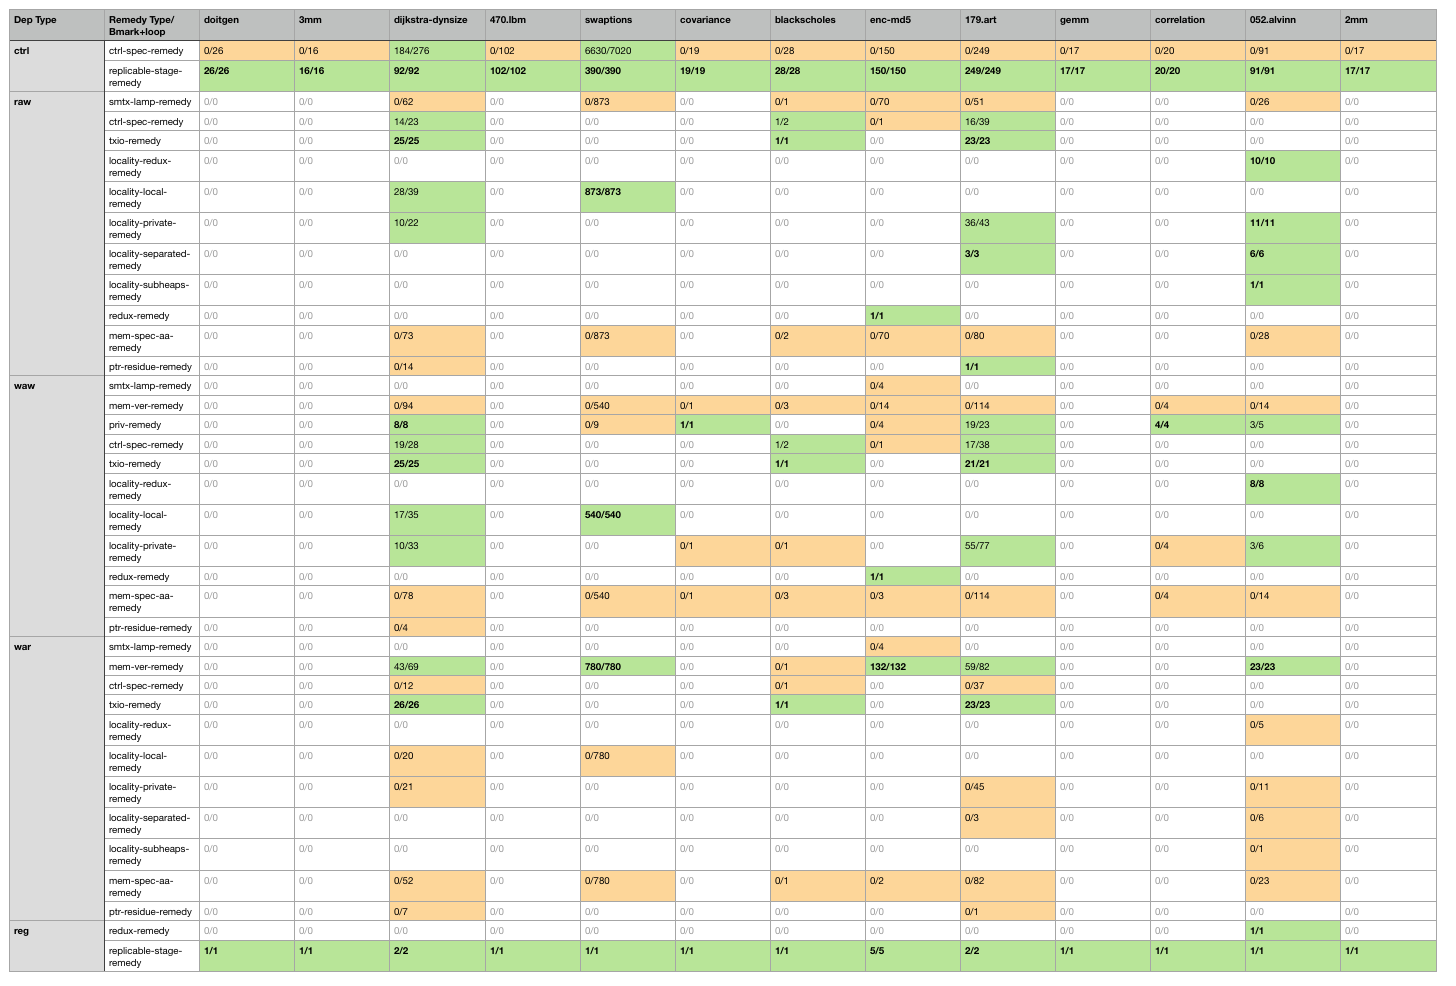
\includegraphics[width=\textwidth]{figures/table.png}
% \label{table:enabler-stats}


% \begin{table}[]
% \label{table:enabler-stats}
% \begin{tabular}{lllllllllllllll}

% Dep Type & Remedy Type/Bmark+loop    & doitgen & 3mm   & dijkstra-dynsize &
% 470.lbm & swaptions & covariance & blackscholes & enc-md5 & 179.art & gemm  &
% correlation & 052.alvinn & 2mm   \\

% ctrl     & ctrl-spec-remedy          & 0/26    & 0/16  & 184/276          &
% 0/102   & 6630/7020 & 0/19       & 0/28         & 0/150   & 0/249   & 0/17  &
% 0/20        & 0/91       & 0/17  \\

%          & replicable-stage-remedy   & 26/26   & 16/16 & 92/92            &
%          102/102 & 390/390   & 19/19      & 28/28        & 150/150 & 249/249 &
%          17/17 & 20/20       & 91/91      & 17/17 \\

% raw      & smtx-lamp-remedy          & 0/0     & 0/0   & 0/62             & 0/0
% & 0/873     & 0/0        & 0/1          & 0/70    & 0/51    & 0/0   & 0/0
% & 0/26       & 0/0   \\
%          & ctrl-spec-remedy          & 0/0     & 0/0   & 14/23            & 0/0
%          & 0/0       & 0/0        & 1/2          & 0/1     & 16/39   & 0/0   &
%          0/0         & 0/0        & 0/0   \\

%          & txio-remedy               & 0/0     & 0/0   & 25/25            & 0/0
%          & 0/0       & 0/0        & 1/1          & 0/0     & 23/23   & 0/0   &
%          0/0         & 0/0        & 0/0   \\

%          & locality-redux-remedy     & 0/0     & 0/0   & 0/0              & 0/0
%          & 0/0       & 0/0        & 0/0          & 0/0     & 0/0     & 0/0   &
%          0/0         & 10/10      & 0/0   \\

%          & locality-local-remedy     & 0/0     & 0/0   & 28/39            & 0/0
%          & 873/873   & 0/0        & 0/0          & 0/0     & 0/0     & 0/0   &
%          0/0         & 0/0        & 0/0   \\

%          & locality-private-remedy   & 0/0     & 0/0   & 10/22            & 0/0
%          & 0/0       & 0/0        & 0/0          & 0/0     & 36/43   & 0/0   &
%          0/0         & 11/11      & 0/0   \\

%          & locality-separated-remedy & 0/0     & 0/0   & 0/0              & 0/0
%          & 0/0       & 0/0        & 0/0          & 0/0     & 3/3     & 0/0   &
%          0/0         & 6/6        & 0/0   \\

%          & locality-subheaps-remedy  & 0/0     & 0/0   & 0/0              & 0/0
%          & 0/0       & 0/0        & 0/0          & 0/0     & 0/0     & 0/0   &
%          0/0         & 1/1        & 0/0   \\

%          & redux-remedy              & 0/0     & 0/0   & 0/0              & 0/0
%          & 0/0       & 0/0        & 0/0          & 1/1     & 0/0     & 0/0   &
%          0/0         & 0/0        & 0/0   \\

%          & mem-spec-aa-remedy        & 0/0     & 0/0   & 0/73             & 0/0
%          & 0/873     & 0/0        & 0/2          & 0/70    & 0/80    & 0/0   &
%          0/0         & 0/28       & 0/0   \\

%          & ptr-residue-remedy        & 0/0     & 0/0   & 0/14             & 0/0
%          & 0/0       & 0/0        & 0/0          & 0/0     & 1/1     & 0/0   &
%          0/0         & 0/0        & 0/0   \\

% waw      & smtx-lamp-remedy          & 0/0     & 0/0   & 0/0              & 0/0
% & 0/0       & 0/0        & 0/0          & 0/4     & 0/0     & 0/0   & 0/0
% & 0/0        & 0/0   \\

%          & mem-ver-remedy            & 0/0     & 0/0   & 0/94             & 0/0
%          & 0/540     & 0/1        & 0/3          & 0/14    & 0/114   & 0/0   &
%          0/4         & 0/14       & 0/0   \\

%          & priv-remedy               & 0/0     & 0/0   & 8/8              & 0/0
%          & 0/9       & 1/1        & 0/0          & 0/4     & 19/23   & 0/0   &
%          4/4         & 3/5        & 0/0   \\

%          & ctrl-spec-remedy          & 0/0     & 0/0   & 19/28            & 0/0
%          & 0/0       & 0/0        & 1/2          & 0/1     & 17/38   & 0/0   &
%          0/0         & 0/0        & 0/0   \\

%          & txio-remedy               & 0/0     & 0/0   & 25/25            & 0/0
%          & 0/0       & 0/0        & 1/1          & 0/0     & 21/21   & 0/0   &
%          0/0         & 0/0        & 0/0   \\

%          & locality-redux-remedy     & 0/0     & 0/0   & 0/0              & 0/0
%          & 0/0       & 0/0        & 0/0          & 0/0     & 0/0     & 0/0   &
%          0/0         & 8/8        & 0/0   \\

%          & locality-local-remedy     & 0/0     & 0/0   & 17/35            & 0/0
%          & 540/540   & 0/0        & 0/0          & 0/0     & 0/0     & 0/0   &
%          0/0         & 0/0        & 0/0   \\

%          & locality-private-remedy   & 0/0     & 0/0   & 10/33            & 0/0
%          & 0/0       & 0/1        & 0/1          & 0/0     & 55/77   & 0/0   &
%          0/4         & 3/6        & 0/0   \\

%          & redux-remedy              & 0/0     & 0/0   & 0/0              & 0/0
%          & 0/0       & 0/0        & 0/0          & 1/1     & 0/0     & 0/0   &
%          0/0         & 0/0        & 0/0   \\

%          & mem-spec-aa-remedy        & 0/0     & 0/0   & 0/78             & 0/0
%          & 0/540     & 0/1        & 0/3          & 0/3     & 0/114   & 0/0   &
%          0/4         & 0/14       & 0/0   \\

%          & ptr-residue-remedy        & 0/0     & 0/0   & 0/4              & 0/0
%          & 0/0       & 0/0        & 0/0          & 0/0     & 0/0     & 0/0   &
%          0/0         & 0/0        & 0/0   \\

% war      & smtx-lamp-remedy          & 0/0     & 0/0   & 0/0              & 0/0
% & 0/0       & 0/0        & 0/0          & 0/4     & 0/0     & 0/0   & 0/0
% & 0/0        & 0/0   \\

%          & mem-ver-remedy            & 0/0     & 0/0   & 43/69            & 0/0
%          & 780/780   & 0/0        & 0/1          & 132/132 & 59/82   & 0/0   &
%          0/0         & 23/23      & 0/0   \\

%          & ctrl-spec-remedy          & 0/0     & 0/0   & 0/12             & 0/0
%          & 0/0       & 0/0        & 0/1          & 0/0     & 0/37    & 0/0   &
%          0/0         & 0/0        & 0/0   \\

%          & txio-remedy               & 0/0     & 0/0   & 26/26            & 0/0
%          & 0/0       & 0/0        & 1/1          & 0/0     & 23/23   & 0/0   &
%          0/0         & 0/0        & 0/0   \\

%          & locality-redux-remedy     & 0/0     & 0/0   & 0/0              & 0/0
%          & 0/0       & 0/0        & 0/0          & 0/0     & 0/0     & 0/0   &
%          0/0         & 0/5        & 0/0   \\

%          & locality-local-remedy     & 0/0     & 0/0   & 0/20             & 0/0
%          & 0/780     & 0/0        & 0/0          & 0/0     & 0/0     & 0/0   &
%          0/0         & 0/0        & 0/0   \\

%          & locality-private-remedy   & 0/0     & 0/0   & 0/21             & 0/0
%          & 0/0       & 0/0        & 0/0          & 0/0     & 0/45    & 0/0   &
%          0/0         & 0/11       & 0/0   \\

%          & locality-separated-remedy & 0/0     & 0/0   & 0/0              & 0/0
%          & 0/0       & 0/0        & 0/0          & 0/0     & 0/3     & 0/0   &
%          0/0         & 0/6        & 0/0   \\

%          & locality-subheaps-remedy  & 0/0     & 0/0   & 0/0              & 0/0
%          & 0/0       & 0/0        & 0/0          & 0/0     & 0/0     & 0/0   &
%          0/0         & 0/1        & 0/0   \\

%          & mem-spec-aa-remedy        & 0/0     & 0/0   & 0/52             & 0/0
%          & 0/780     & 0/0        & 0/1          & 0/2     & 0/82    & 0/0   &
%          0/0         & 0/23       & 0/0   \\

%          & ptr-residue-remedy        & 0/0     & 0/0   & 0/7              & 0/0
%          & 0/0       & 0/0        & 0/0          & 0/0     & 0/1     & 0/0   &
%          0/0         & 0/0        & 0/0   \\

% reg      & redux-remedy              & 0/0     & 0/0   & 0/0              & 0/0
% & 0/0       & 0/0        & 0/0          & 0/0     & 0/0     & 0/0   & 0/0
% & 1/1        & 0/0   \\

%          & replicable-stage-remedy   & 1/1     & 1/1   & 2/2              & 1/1
%          & 1/1       & 1/1        & 1/1          & 5/5     & 2/2     & 1/1   &
%          1/1         & 1/1        & 1/1
% \end{tabular}
% \end{table}

% Discussion of the table



 % !TEX root = paper.tex
\section{Evaluation}
\label{eval}
\name is evaluated on a commodity shared-memory machine with two 14-core
Intel Xeon CPU E5-2697 v3 processors (28 cores total) running at 2.60GHz
(turbo-boost disabled) with 756GB of memory. The operating system is
64-bit Ubuntu 16.04.5 LTS with GCC 5.5 (version 5.5.0 20171010).
\namensp's compiler is implemented on the LLVM Compiler Infrastructure
(version 5.0.2)\cite{LLVM:CGO04}.


\name is evaluated against 12 C and C++ benchmarks, covering all the
parallelizable (exhibiting speedup) benchmarks from two
state-of-the-art automatic speculative-DOALL parallelization
papers (Privateer~\cite{johnson:12:pldi}, Cluster
Spec-DOALL~\cite{kim:12:cgo}) as well as an additional benchmark
(179.art) from HELIX~\cite{simone:12:cgo}, a non-speculative automatic
parallelization system.
We choose benchmarks that have been parallelized in prior work because this
work is focused on boosting the efficiency of automatic parallelization
rather than increasing its applicability.

% These benchmarks are from five benchmark suites (SPEC\cite{},
% PARSEC\cite{bienia:08:parsec}, PolyBench\cite{},
% MiBench\cite{guthaus:2001:iiwsc}, Trimaran\cite{trimaran:web}).
We modify the benchmarks from Polybench and \texttt{dijkstra} from
MiBench to dynamically allocate previously statically allocated arrays in order to accept
command line-defined sizes in the same way as ~\cite{johnson:12:pldi, kim:12:cgo}.
% All PolyBench benchmarks and \texttt{dijkstra} from MiBench are modified
% to accept command line arguments and allocate arrays dynamically in
% the same way as in~\cite{johnson:12:pldi, kim:12:cgo}.
%This modification is used to create bigger inputs, necessary for
%separating profiling and evaluation input sets.
%
%for exhibiting speedups on 28 cores
%
Benchmarks are profiled using small inputs, while all the
experiments presented in this section are conducted using different,
large evaluation inputs. The evaluation inputs are chosen to be large
enough for the sequential version to run for at least 10 minutes to
observe accurate parallel execution times on 28 cores. Reported speedups
are an average of 5 runs to minimize the effect of the variance in execution
time that manifests between runs.


\begin{table*}[h]
  \centering
  % !TEX root = ../paper.tex
\small
\centering
\begin{tabular}{|l|c|c|l|l|}
\hline
Benchmarks & DOALL Coverage & Sequential Time & Arguments & Input    \\
\hline
doitgen    & 99.6\%  & 1034.86 & 768 768 768 & -  \\
\hline
enc-md5    & 100.0\% & 174.26    & 1000 & -  \\
\hline
covariance & 99.9\%  &     & 4096 4096 & -  \\
\hline
swaptions  & 100.0\% & 1546.29   & -ns 10000 -sm 40000 -nt 1 & -  \\
\hline
3mm  & 100.0\%       & 3515.78   & 4096 4096 4096 4096 4096                & -  \\
\hline
gemm       & 100.0\% & 1182.50   & 4096 4096 4096                    & -  \\
\hline
179.art    & 99.1\%  & 702.32    &
{\parbox[l]{5cm}{-scanfile c756hel.in \\-trainfile1 a10.img \\-trainfile2 hc.img\\ -stride 1 -startx 60 \\-starty 90 -endx 210 \\ -endy 240 -objects 10}} & input1   \\
\hline
dijkstra-dynsize & 99.7\%  &     & ../input3000/input3000.in 3000                & input300 \\
\hline
blackscholes & 99.7\% & 4702.20   & 1 in\_10M.txt out\_10M.txt                & ref      \\
\hline
2mm  & 100.0\%       & 2360.60   & 4096 4096 4096 4096               & -  \\
\hline
052.alvinn & 97.5\%  &     & 60000                 & input 1  \\
\hline
correlation & 99.7\%  & 914.39    & 4096 4096                   & - \\
\hline
\end{tabular}
  \caption{
    Benchmark Details:
    (A) Percentage of
    execution time spent inside the parallelized loop(s) compared to
    that of the whole program. The theoretical speedup
    is calculated using Amdahl's Law with the assumptions of no overheads and
    running with 28 workers.
    (B) Number and percentage of cross-iteration dependences
    handled by Speculation-Aware Memory Analyzer (SAMA) that were unresolved by
    static analysis alone. Entries denotes by
    ``N/A'' indicate all dependences are handled by static analysis.
    (C) Number and percentage of objects covered by efficient speculative
    privatization transformations proposed
    in this work.
    (D) Private read and write sizes measured using the
    test input for each benchmark; v1 represents
    \name with only the planner; v2 represents \name with
    the planner and propsed enablers.}
  \label{tab:benchmark-list}
    \vspace{-5pt}
\end{table*}

\subsection{Parallelization Performance}

\begin{figure*}[ht]
  \centering
  \resizebox{0.90\textwidth}{!}{
  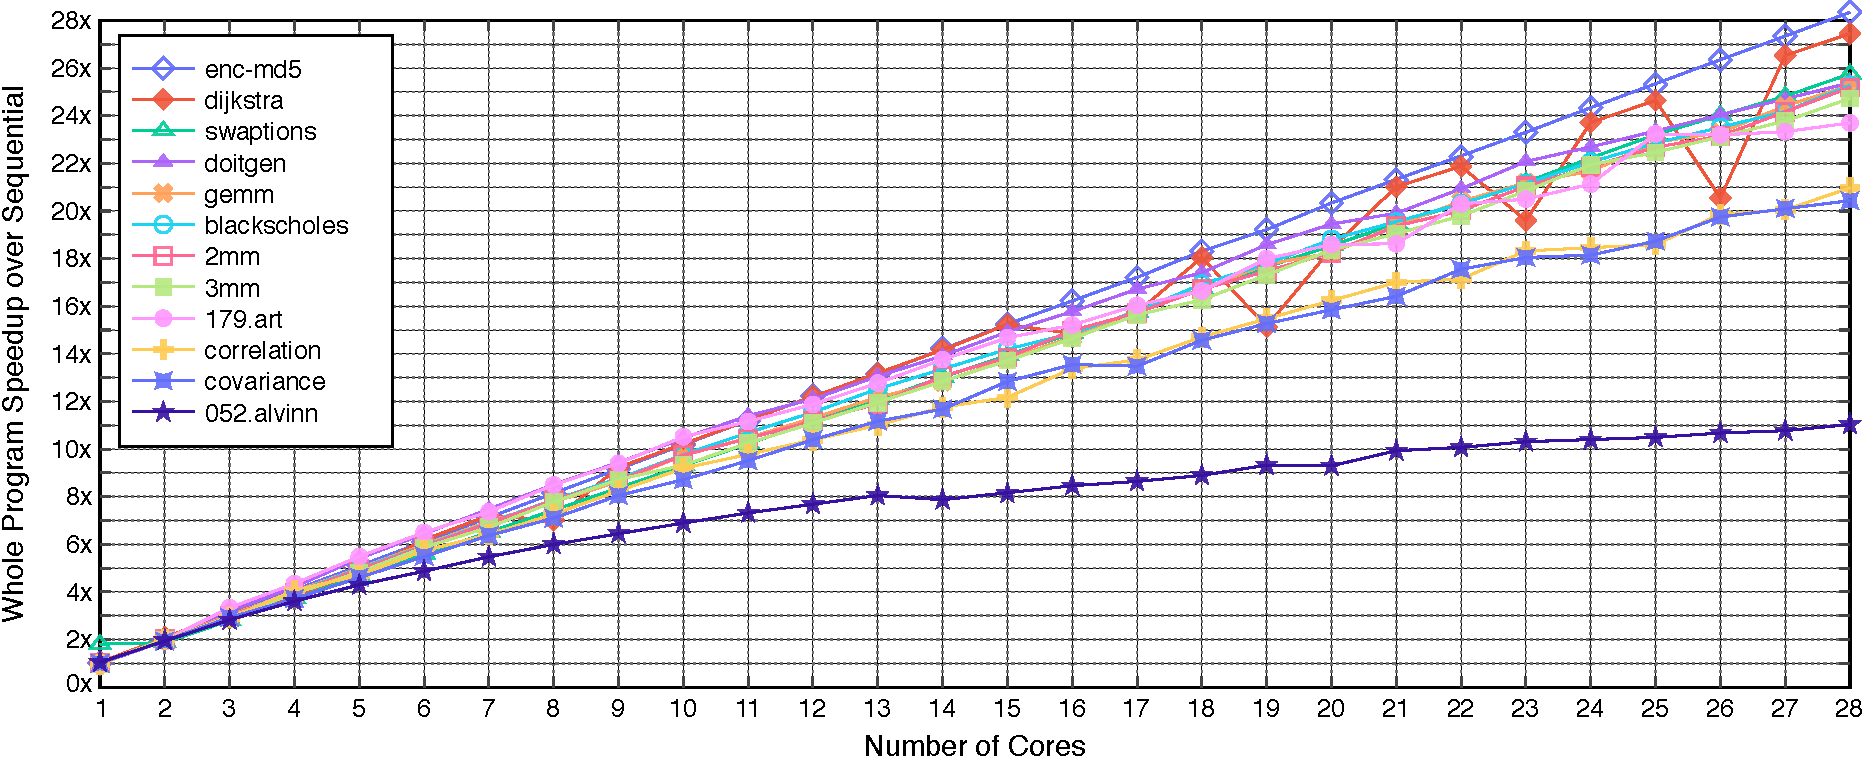
\includegraphics[width=\textwidth]{figures/multi-core-crop}
  }
  \caption{Fully Automatic Whole Program Speedup over Sequential}
  \label{fig:multi-core-scale}
\end{figure*}

Figure \ref{fig:multi-core-scale} presents whole program speedups for
all benchmarks running on one (1) to 28 cores. These speedups are
relative to the sequential performance of the original code, compiled
with \texttt{clang++ -O3}. \name achieves scalable performance on all the
benchmarks due to the overhead reduction resulting from the use
of SAMA and the new enablers. Figure \ref{fig:speedup-compare} compares \namensp's results
with Privateer and two variant of \namensp with various components disabled.

The first bar shows the performance of Privateer implemented with best practices.
% Peephole optimizations are used to reduce the use of memory
% speculation and to hoist and combine memory checks out of the inner loop(s).
The speedup and runtime breakdown results are comparable to those reported
in the paper. Although a state-of-the-art framework in terms of applicability,
Privateer misses opportunities to remove read checks as mentioned in
STMLite\cite{mehrara:09:stmlite} and Cluster Spec-DOALL\cite{kim:12:cgo}.
For non-speculatively parallelized benchmarks especially, Privateer does not use
static analysis and as a result has unnecessarily large read and write
sets.
%

The second bar demonstrates the effect of using information from static
analysis, profiling, and transformations to infer unnecessary reads in the
case of objects privatized without the use of speculation. We notice
that \texttt{2mm}, \texttt{3mm}, \texttt{doitgen}, \texttt{enc-md5}, and
\texttt{179.art} benefit from this improvement. (D) in Table
\ref{tab:benchmark-list} reveals that for \texttt{doitgen} and \texttt{3mm},
the read set size is reduced from 2.53TB and 3TB, respectively, to zero.
The absence of these reads also allows monitoring of writes to the same
location inside the loop to be hoisted outside the loop, further decreasing
the overhead.
% To
% improve upon Privateer, we utilize static analysis
% including a stronger KillFlow analysis pass to remove read checks.
% \texttt{2mm}, \texttt{3mm}, \texttt{doitgen}, \texttt{enc-md5}, and
% \texttt{179.art} benefit from this improvement as shown in the second bar.
% Note that \textbf{ref XXX} if all dependences are removed statically, no
% checkpoint is needed in the runtime.
%

The third bar shows how the addition of the enablers proposed in section
\ref{novel_transf} to the planner affects performance. These enablers
avoid adding expensive monitoring of writes taking into account specific
properties of memory objects. \texttt{2mm} and \texttt{3mm} have loops in
which each iteration writes to a different location in a privatized array.
Since this is determined statically, we can refrain from monitoring any of
these writes. In \texttt{blackscholes}, the \texttt{\textbf{prices}} array
is fully overwritten at every iteration; therefore, we only need to take
the last iteration's writes as the liveout. In \texttt{dijkstra},
the \texttt{\textbf{pathcost}} array is killed at the beginning of each
iteration and similar to \texttt{blackscholes}, only requires the last
iteration's writes to be known.

The last bar illustrates the performance of adding the speculation-aware
memory analyzer to the list of features. The main performance benefit of
this is seen with \texttt{dijkstra}, where the read check of
\texttt{\textbf{dist}} is removed. Using control speculation in conjunction
with kill-flow analysis can remove the RAW dependence between lines
\textbf{14} and \textbf{38}, which is unremovable with static analysis
alone or using static analysis after control speculation is applied.
% XXX Should we talk about why or is this explained earlier in the paper?
The remaining 3.61KB of monitored writes results from a cross-iteration
register dependence of the induction variable, which is logged every
iteration before a checkpoint.

\texttt{covariance} and \texttt{correlation} have complex WAW dependences
that cannot be resolved even with SAMA and the write sets need to be
monitored, limiting the achievable speedup to 20.5$\times$ and 21$\times$,
respectively.

% \texttt{179.art}


Using SAMA addresses dependences not covered by static analysis in
\texttt{enc-md5}, \texttt{179.art}, \texttt{blackscholes}, and
\texttt{dijkstra}, shown in (B) of Table ~\ref{tab:benchmark-list}. However,
many of these dependences are in the outer loops (with the exception
being \texttt{dijkstra}) and do not affect the overall performance much.
Nevertheless, this approach is worth exploring further in future work.
% XXX Better wording for this.

% The third bar presents the results of \name without the cheap
% privatization transformations proposed in \ref{}. Parallelization through
% \name, which incorporates speculation-aware-memory-analysis and cheap
% privatization transformations, is presented in the fourth bar, achieving
% 23.0$\times$ speedup compared to 11.5$\times$ by the original Privateer.

% enc-md5, swaptions, gemm, 3mm, 2mm, blackscholes, doitgen
% We observe close to linear scalability for \texttt{enc-md5}, \texttt{swaptions},
% \texttt{gemm}, \texttt{2mm}, \texttt{3mm}, \texttt{blackscholes},
% and \texttt{doitgen}. This performance comes from most memory
% objects being privatized with little or no overheads.

% dijkstra
% \texttt{dijkstra}, having many calls to \texttt{\textbf{malloc()}}
% inside the inner loops, shows a significant variance in
% the runtime.

% 052.alvinn
% \texttt{052.alvinn} exhibits a lower speedup (11$\times$ on 28
% cores) than other the benchmarks, resulting from the inner loop
% being chosen for parallelization. With this loop constituting 97.5\% of the
% execution time of the whole program, the theoretical max speedup is 16.7$\times$
% based on Almdahl's Law.

% 179.art
% \texttt{179.art}, whose theoretical maximum speedup is 22.5$\times$, due to
% the same effect. Note that HELIX\cite{simone:12:cgo} reports 4.2$\times$ speedup
% on 6 cores while \name exhibits 6.5$\times$, demonstrating that an efficient
% speculative approach can outperform even a static approach.

% correlation and covariance
% \texttt{correlation} and \texttt{covariance} have WAW
% dependence patterns which cannot be resolved by static analysis or cheap
% privatization variants. As a result, the corresponding memory objects are
% classified as private and need logging and merging for write sets,
% resulting in lower speedups.

\begin{figure*}[ht]
  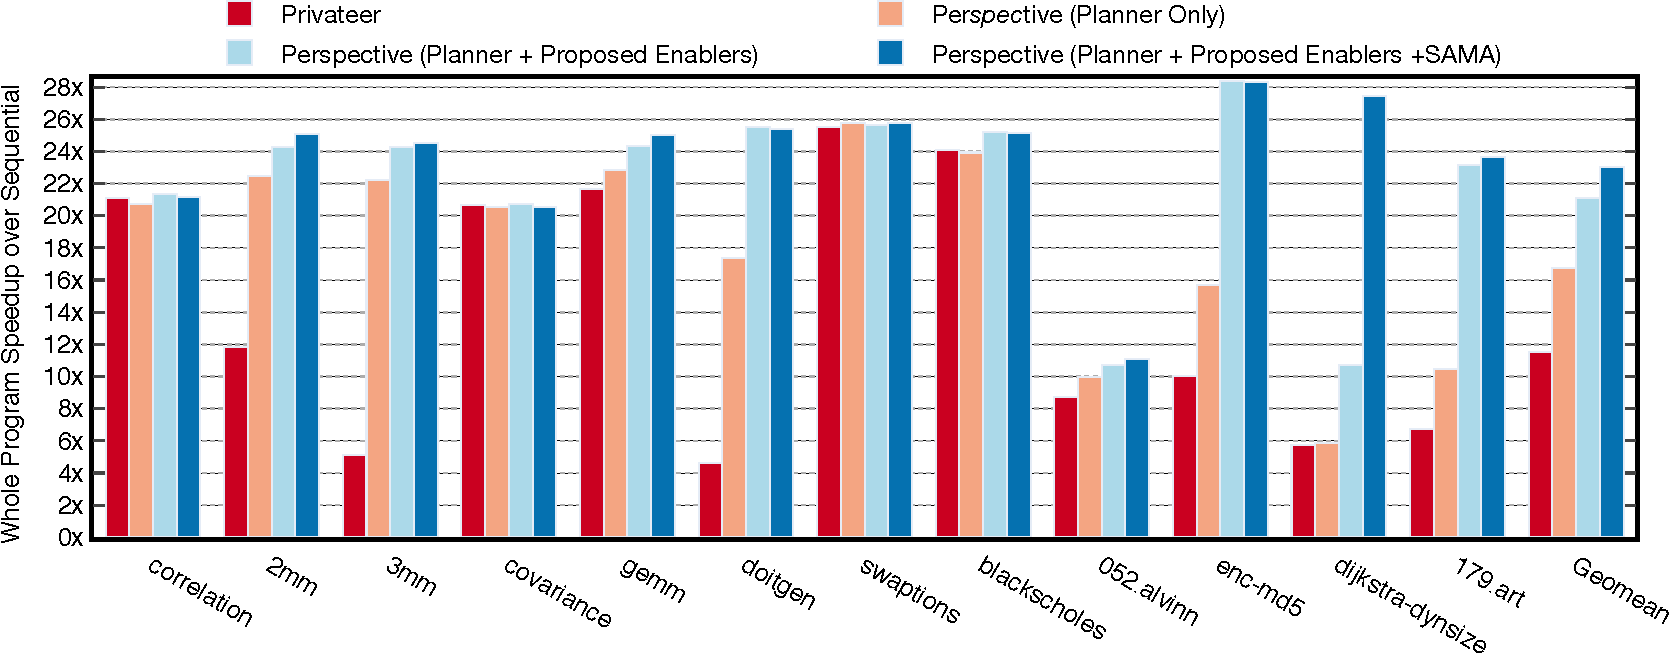
\includegraphics[width=\textwidth]{figures/compare-privateer}
  \caption{Whole Program Speedup Comparison among variants of \name and Privateer with 28 Cores}
  \label{fig:speedup-compare}
\end{figure*}



% \subsubsection{Effect of parallelization on vectorization}

% instrumentation kills vectorization


% \subsection{Static Analysis and Enablers}
% Figures Needed:
% \begin{itemize}
% % (no need, just discuss the use of CAF in previous sections) \item CAF:
% % with and without; no topping; with only BasicLoopAA and ScevAA

% % (no need, show in the benchmark table) \item Coverage: Spec-DOALL
% % percentage of coverage of each benchmark
% \item Enablers: Enablers used for each benchmark
% \item Optimization level: Performance with different optimization levels
% \end{itemize}

% Discussion Needed:

% Present in a table, which enablers were used for all benchmarks

\subsection{Aspects Affecting Performance}
% XXX Better wording of this

% \begin{figure*}[htp]
%   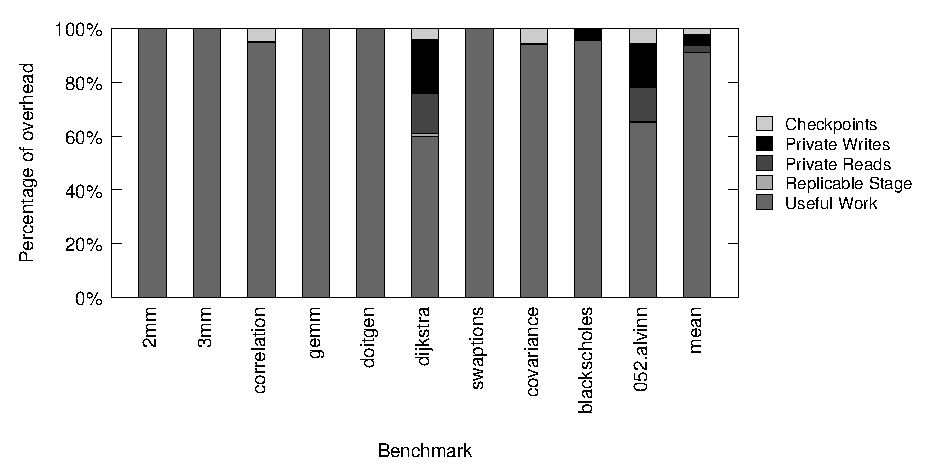
\includegraphics[width=0.9\textwidth]{figures/overheads}
%   \label{fig:overheads}
%   \caption{Overhead comparison with various enablers disabled}
% \end{figure*}
% \begin{figure*}[htp]
%   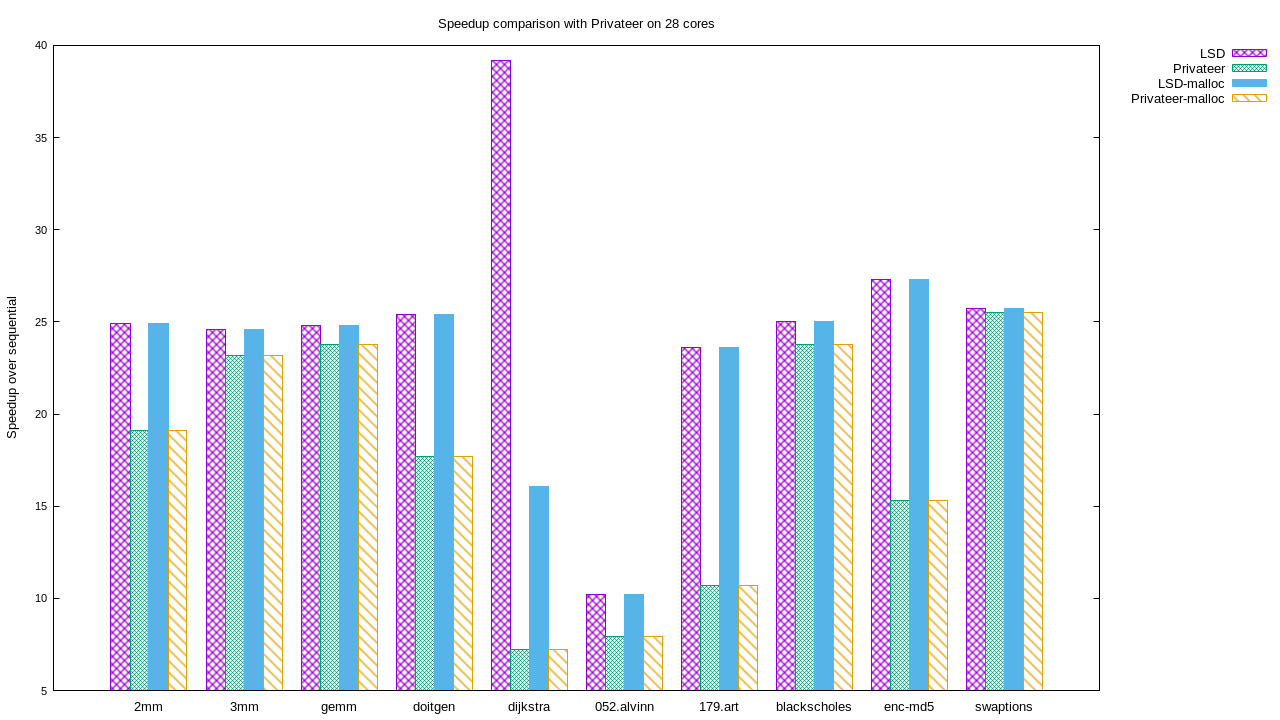
\includegraphics[width=0.9\textwidth]{figures/comparison}
% \end{figure*}
% Huge speedup for dijkstra is largely due to the cheaper "malloc" that
% we use in our heaps. Using a similar malloc in the sequential version
% yields ~16x speedup in dijkstra and insignificant difference in the
% other benchmarks.
% Shown in Figure \ref{fig:overheads} is the overhead breakdown of each
% benchmark comparing \name with various enablers disabled. The useful work
% of \name is normalized to 100\%, with the others being scaled accordingly.
% These result demonstrate the correlation between the sum of the overheads
% to the speedup that can be achieved. \{\textbf{XXX} Something about
% how we remove dependences with redundant private read elimination,
% the new kill\_private heap, and collaboration \}

Along with adding its own overheads, the instrumentation inserted to monitor
reads and writes can also disable other optimizations, such as
vectorization. The use of vectorization in \texttt{052.alvinn} yields 30\%
speedup in the sequential execution. With logging of arbitrary addresses, the loop
vectorizer of LLVM cannot infer that these do not alias with any other
pointer of a previously vectorizable instruction.
% XXX Is this worded horribly? Too wired to tell now

For most of the benchmarks, checkpointing does not add any
significant (>1\%) overhead; the exceptions are
\texttt{052.alvinn}, \texttt{correlation}, and \texttt{covariance}.
The inner loop of \texttt{052.alvinn} is chosen for parallelization --
because the useful work of the loop is small and runs for 60,000
iterations, checkpointing constitutes a considerable portion of the run
time, \textasciitilde20\%. For \texttt{covariance} and \texttt{correlation},
the speculation-aware memory analyzer could not avoid using memory
speculation and as such, the checkpoints need to merge large private sets
with an overhead of \textasciitilde10\% for each.

For several benchmarks, we observed speedups that exceed their theoretical
limits, which we attribute to two factors:
(1) we replace all calls to \texttt{\textbf{malloc()}} inside a parallelized
loop with our own heap allocator. Our implementation of this allocator
does not track segments of memory that have been freed for later use in the
way most C/C++ runtime libraries do and as such, the overhead for dynamic
(de)allocation is drastically reduced, which is seen in \texttt{dijkstra}.
(2) using multiple cores increases the effective cache size which may
reduce access times to memory~\cite{jeon:11:oopsla}. This effect can be
seen in the performance of \texttt{179.art}, \texttt{enc-md5}, and
\texttt{doitgen}.

\subsection{Misspeculation Evaluation}
\begin{figure}[htp]
  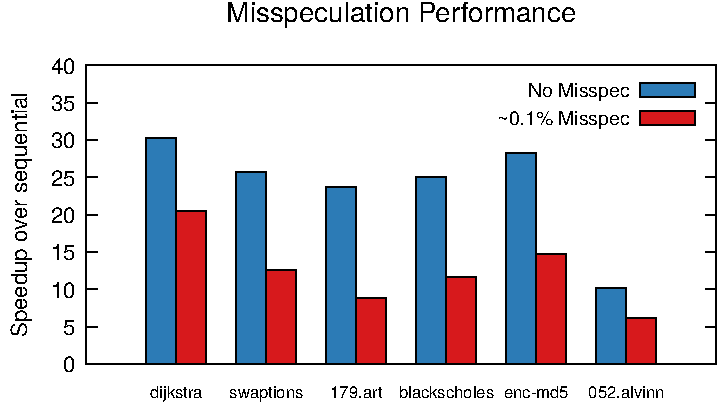
\includegraphics[width=\columnwidth]{figures/misspec-crop}
  \caption{Misspeculation performance across speculative benchmarks}
  \label{fig:misspec}
\end{figure}
Figure \ref{fig:misspec} shows how misspeculation affects the
performance of the six speculative benchmarks with a misspeculation rate of
0.1\%. Since none of the benchmarks exhibit misspeculation on the
given input sets, we artificially inject misspeculation at the end of
every 1000 iterations to observe the performance degradation.
Note that for many benchmarks, speculation is only used
because analysis cannot disprove a dependence, even though manually
examining the source code reveals that the dependence will never manifest.
Thus, the only place misspeculation can possibly occur is during a heap
check.
% Note that misspeculation with \name is extremely unlikely, as
% static analysis can disprove many speculative assumptions and for many of
% the benchmarks, misspeculation is only possible during a heap check.
The inputs for \texttt{179.art} were not large enough to have
enough iterations for misspeculation at this rate, so we perform a
weighted average of non-misspeculating and misspeculating runs to achieve
an average corresponding to the respective rate.
These results demonstrate that \name performs well with only high
confidence speculation and requires tight integration with static analysis
to avoid heavy-weight speculation whenever possible.
Systems that have larger overheads have a larger chance of speculation (since
they use more speculative assumptions), but we minimize the amount of speculation.
\{\textbf{XXX} Reword this\}
% As the iteration within a checkpoint that misspeculation
% occurs can affect the recovery cost, we inject these misspeculations in the
% middle of a checkpoint chunk (\textbf{XXX} find better wording) to have a more
% realistic simulation, assuming that programs can misspeculate at any iteration with a
% uniform distribution.

% \subsection{Power Consumption}

% Power and energy stats here


 \section{Related Work}

% For non-spec DOALL-only compilers: with only static analysis, the
% struggle is the applicability (maybe plus the cost of logging and merging
% live-outs (copy-outs)); with runtime checks (predicates), the focus is
% the applicability and extraction of efficient runtime checks.

% For compilers using different techniques than DOALL: communication of
% real dependences is needed. The overheads can be broken down to
% communication cost, lost cycles due to imbalance.

% For Spec DOALL-only compilers: with memory speculation, the applicability
% is perfect, meaning all “real” DOALL loops can be handled by just
% ignoring dependences that can not be disproved but will never or seldom
% manifest in runtime. The overheads include speculation validation cost,
% misspeculation recovery cost, and the cost of logging & merging
% (maintaining) live-outs.

% For systems with special hardware support: for example, with
% transactional memory systems, the memory versioning of main memory is
% there implicitly. Assuming you have a transactional memory system with
% zero time overhead, what you need to do is just spawning the iterations,
% false dependences including anti- and output- dependences are avoided,
% when one iteration has a real dependences (flow) to its previous
% iteration but executes earlier, the memory system can stall it when it
% tries to load the pending value. However, the assumption of 0-overhead TM
% systems is not possible.

% \paragraph{Analysis-based Parallelization System}
% % Polaris
% % SUIF
% % HELIX
% % DSWP (non spec version)
% % Hybrid Analysis
% % Sensitivity Analysis

Early non-speculative parallelizing compilers (Polaris, SUIF) based on
DOALL paradigm use static analysis to disprove dependences and run-time
analysis to extract predicate for dynamic privatization. These systems work
well with regular scientific programs and exhibit good speedup when
applicable. However, when dealing with general purpose programs, they are
limited by imprecise static analysis and heavyweight run-time analysis.
They also lack in support for dynamically allocated memory objects, which
are widely used in modern programming. Recent works on non-speculative
parallelization (HELIX~\cite{simone:12:cgo}, DOCyclical~\cite{yu2016cyclical}, DSWP~\cite{ottoni:05:micro}, and PS-DSWP~\cite{raman:08a:cgo}) focus more on alternative
parallelization paradigms like DOACROSS and DOPIPE, which allow
communication of flow dependences among cores. \name focuses on DOALL but
the contributions of this work are complementary with other parallelization
paradigms. LRPD leverages speculation to evaluate privatization criterion,
extends the applicability of DOALL. Yet it is still limited to array-based
objects.

STMlite, CorD, and Privateer use speculation extensively to privatize
objects for general purpose programs. As mentioned in Privateer, STMlite
and CorD don't support speculative reduction, and limit the applicability
to static cases. Privateer, by introducing heap separation and doin
aggressive speculative privatization, achieves the state-of-the-art
applicability. However, it fails to recognize a lot of optimization
opportunities and suffers from the two major overhead mentioned in
\ref{sec:motivation}.

Recent work~\cite{ctian:2008:micro,johnson:12:pldi,kim:12:cgo} avoids some
memory speculations by speculating higher-level properties like local
objects whose validation does not require logging or communication.
Sensitivity Analysis~\cite{Rus:07:ics} uses a cascade design of run time
tests to generate predicates for memory dependences, which reduce the
run-time overhead. Yet, all of these optimization efforts are rudimentary
compared to \namensp.

Another line of work extracts parallelism among loop iterations by ignoring data dependences rather than speculating their non-existence~\cite{campanoni:2015:cgo,Udupa:2011:AEB:1993498.1993555,misailovic2013parallelizing}.
These approaches extract parallelism sacrificing the program's output quality.
Instead, \name extracts parallelism while guaranteeing the preservation of the original output quality.

Finally, some recent work speculate on properties of data dependences like commutativity~\cite{kulkarni:07:pldi,Nguyen:2014:DGO:2541940.2541964} and having short memory~\cite{Deiana:2018:UPN:3173162.3173181}.
These techniques involve heavy speculation and they require developers to cast programs in specialized code patterns expected by their compilers and runtimes.
Instead, \name parallelization is transparent to developers allowing them to write their code to target their specific goals (e.g., productivity, maintainability, integrability).

% HELIX
% The HELIX parallelizing compiler extracts TLP by distributing loop
% iterations between cores within the same chip. HELIX is a generalization of
% DOACROSS and DOALL techniques for modern multicore architectures and,
% therefore, HELIX-parallelized loops include DOALL ones. HELIX does not rely
% on speculation to avoid the related overhead, which limits the approach to
% target only medium and small loops (where the accuracy of code analyses is
% higher) for most benchmarks. Targeting such loops increases the
% communication demand, which makes HELIX particularly appealing when coupled
% with an architecture support designed to accelerate core-to-core
% communication. On the other hand, LSD decreases the speculation overhead
% enough to make DOALL parallelization practical on existing commodity
% multicores.

% Parallelization with Programmers' Support
% Paralax


% \paragraph{Speculative Parallelization System:}


% \paragraph{Software transactional memory system:}

% Other work on software transactional memory tried to reduce the overhead by
% using some extent of static analysis or/and privatization (STMlite, CorD).


% \paragraph{Attempts to Reduce Runtime Overheads}




 \section{Conclusion}

This paper identifies and mitigates core inefficiencies of prior
automatic speculative-DOALL systems. \name combines a novel
speculation-aware memory analyzer, efficient variants of speculative
privatization and a modular planning phase to generate minimal cost
parallelization plans, avoiding overheads of prior work.
%
\name fully-automatically yields geomean whole-program speedup of
23.0$\times$ over sequential execution for 12 C/C++ benchmarks on a
28-core shared memory machine, whereas Privateer, the most applicable
prior automatic speculative-DOALL system achieves 11.5$\times$ geomean
speedup.

The modularity of the proposed compiler design allows easy
extensibility with additional speculative assumptions and enabling
transformations.
This framework could also be extended for parallelization paradigms
beyond DOALL.


 \bibliographystyle{plain}
 \bibliography{references}


 \end{document}
